\PassOptionsToPackage{unicode=true}{hyperref} % options for packages loaded elsewhere
\PassOptionsToPackage{hyphens}{url}
%
\documentclass[]{book}
\usepackage{lmodern}
\usepackage{amssymb,amsmath}
\usepackage{ifxetex,ifluatex}
\usepackage{fixltx2e} % provides \textsubscript
\ifnum 0\ifxetex 1\fi\ifluatex 1\fi=0 % if pdftex
  \usepackage[T1]{fontenc}
  \usepackage[utf8]{inputenc}
  \usepackage{textcomp} % provides euro and other symbols
\else % if luatex or xelatex
  \usepackage{unicode-math}
  \defaultfontfeatures{Ligatures=TeX,Scale=MatchLowercase}
\fi
% use upquote if available, for straight quotes in verbatim environments
\IfFileExists{upquote.sty}{\usepackage{upquote}}{}
% use microtype if available
\IfFileExists{microtype.sty}{%
\usepackage[]{microtype}
\UseMicrotypeSet[protrusion]{basicmath} % disable protrusion for tt fonts
}{}
\IfFileExists{parskip.sty}{%
\usepackage{parskip}
}{% else
\setlength{\parindent}{0pt}
\setlength{\parskip}{6pt plus 2pt minus 1pt}
}
\usepackage{hyperref}
\hypersetup{
            pdftitle={Introdução a análise de dados ambientais em R},
            pdfauthor={Wilson Souza \& Thiago Couto},
            pdfborder={0 0 0},
            breaklinks=true}
\urlstyle{same}  % don't use monospace font for urls
\usepackage{color}
\usepackage{fancyvrb}
\newcommand{\VerbBar}{|}
\newcommand{\VERB}{\Verb[commandchars=\\\{\}]}
\DefineVerbatimEnvironment{Highlighting}{Verbatim}{commandchars=\\\{\}}
% Add ',fontsize=\small' for more characters per line
\usepackage{framed}
\definecolor{shadecolor}{RGB}{248,248,248}
\newenvironment{Shaded}{\begin{snugshade}}{\end{snugshade}}
\newcommand{\AlertTok}[1]{\textcolor[rgb]{0.94,0.16,0.16}{#1}}
\newcommand{\AnnotationTok}[1]{\textcolor[rgb]{0.56,0.35,0.01}{\textbf{\textit{#1}}}}
\newcommand{\AttributeTok}[1]{\textcolor[rgb]{0.77,0.63,0.00}{#1}}
\newcommand{\BaseNTok}[1]{\textcolor[rgb]{0.00,0.00,0.81}{#1}}
\newcommand{\BuiltInTok}[1]{#1}
\newcommand{\CharTok}[1]{\textcolor[rgb]{0.31,0.60,0.02}{#1}}
\newcommand{\CommentTok}[1]{\textcolor[rgb]{0.56,0.35,0.01}{\textit{#1}}}
\newcommand{\CommentVarTok}[1]{\textcolor[rgb]{0.56,0.35,0.01}{\textbf{\textit{#1}}}}
\newcommand{\ConstantTok}[1]{\textcolor[rgb]{0.00,0.00,0.00}{#1}}
\newcommand{\ControlFlowTok}[1]{\textcolor[rgb]{0.13,0.29,0.53}{\textbf{#1}}}
\newcommand{\DataTypeTok}[1]{\textcolor[rgb]{0.13,0.29,0.53}{#1}}
\newcommand{\DecValTok}[1]{\textcolor[rgb]{0.00,0.00,0.81}{#1}}
\newcommand{\DocumentationTok}[1]{\textcolor[rgb]{0.56,0.35,0.01}{\textbf{\textit{#1}}}}
\newcommand{\ErrorTok}[1]{\textcolor[rgb]{0.64,0.00,0.00}{\textbf{#1}}}
\newcommand{\ExtensionTok}[1]{#1}
\newcommand{\FloatTok}[1]{\textcolor[rgb]{0.00,0.00,0.81}{#1}}
\newcommand{\FunctionTok}[1]{\textcolor[rgb]{0.00,0.00,0.00}{#1}}
\newcommand{\ImportTok}[1]{#1}
\newcommand{\InformationTok}[1]{\textcolor[rgb]{0.56,0.35,0.01}{\textbf{\textit{#1}}}}
\newcommand{\KeywordTok}[1]{\textcolor[rgb]{0.13,0.29,0.53}{\textbf{#1}}}
\newcommand{\NormalTok}[1]{#1}
\newcommand{\OperatorTok}[1]{\textcolor[rgb]{0.81,0.36,0.00}{\textbf{#1}}}
\newcommand{\OtherTok}[1]{\textcolor[rgb]{0.56,0.35,0.01}{#1}}
\newcommand{\PreprocessorTok}[1]{\textcolor[rgb]{0.56,0.35,0.01}{\textit{#1}}}
\newcommand{\RegionMarkerTok}[1]{#1}
\newcommand{\SpecialCharTok}[1]{\textcolor[rgb]{0.00,0.00,0.00}{#1}}
\newcommand{\SpecialStringTok}[1]{\textcolor[rgb]{0.31,0.60,0.02}{#1}}
\newcommand{\StringTok}[1]{\textcolor[rgb]{0.31,0.60,0.02}{#1}}
\newcommand{\VariableTok}[1]{\textcolor[rgb]{0.00,0.00,0.00}{#1}}
\newcommand{\VerbatimStringTok}[1]{\textcolor[rgb]{0.31,0.60,0.02}{#1}}
\newcommand{\WarningTok}[1]{\textcolor[rgb]{0.56,0.35,0.01}{\textbf{\textit{#1}}}}
\usepackage{longtable,booktabs}
% Fix footnotes in tables (requires footnote package)
\IfFileExists{footnote.sty}{\usepackage{footnote}\makesavenoteenv{longtable}}{}
\usepackage{graphicx,grffile}
\makeatletter
\def\maxwidth{\ifdim\Gin@nat@width>\linewidth\linewidth\else\Gin@nat@width\fi}
\def\maxheight{\ifdim\Gin@nat@height>\textheight\textheight\else\Gin@nat@height\fi}
\makeatother
% Scale images if necessary, so that they will not overflow the page
% margins by default, and it is still possible to overwrite the defaults
% using explicit options in \includegraphics[width, height, ...]{}
\setkeys{Gin}{width=\maxwidth,height=\maxheight,keepaspectratio}
\setlength{\emergencystretch}{3em}  % prevent overfull lines
\providecommand{\tightlist}{%
  \setlength{\itemsep}{0pt}\setlength{\parskip}{0pt}}
\setcounter{secnumdepth}{5}
% Redefines (sub)paragraphs to behave more like sections
\ifx\paragraph\undefined\else
\let\oldparagraph\paragraph
\renewcommand{\paragraph}[1]{\oldparagraph{#1}\mbox{}}
\fi
\ifx\subparagraph\undefined\else
\let\oldsubparagraph\subparagraph
\renewcommand{\subparagraph}[1]{\oldsubparagraph{#1}\mbox{}}
\fi

% set default figure placement to htbp
\makeatletter
\def\fps@figure{htbp}
\makeatother

\usepackage{booktabs}
\usepackage{booktabs}
\usepackage{longtable}
\usepackage{array}
\usepackage{multirow}
\usepackage{wrapfig}
\usepackage{float}
\usepackage{colortbl}
\usepackage{pdflscape}
\usepackage{tabu}
\usepackage{threeparttable}
\usepackage{threeparttablex}
\usepackage[normalem]{ulem}
\usepackage{makecell}
\usepackage{xcolor}
\usepackage[]{natbib}
\bibliographystyle{apalike}

\title{Introdução a análise de dados ambientais em R}
\author{Wilson Souza \& Thiago Couto}
\date{2020-11-18}

\begin{document}
\maketitle

{
\setcounter{tocdepth}{1}
\tableofcontents
}
\hypertarget{prefuxe1cio}{%
\chapter*{Prefácio}\label{prefuxe1cio}}
\addcontentsline{toc}{chapter}{Prefácio}

In this book, we will introduce an interesting

\hypertarget{sobre-os-autores}{%
\chapter*{Sobre os autores}\label{sobre-os-autores}}
\addcontentsline{toc}{chapter}{Sobre os autores}

\textbf{Wilson Souza}

Possui graduação em Licenciatura em Ciências Biológicas pela Universidade Federal do Rio de Janeiro com dupla diplomação com a Universidade de Coimbra - Portugal, Bacharelado em Biologia Marinha pela Universidade Federal do Rio de Janeiro e Mestrado em Oceanografia Biológica pela Universidade Federal do Rio Grande. Desde 2012 trabalha em projetos de monitoramento de populações de camarões com foco em aspectos ecológicos e pesqueiros e em projetos de ecologia de benthos marinho. Aprendeu a linguagem R durante o mestrado e desde então tem se dedicado a ampliar seus conhecimentos em bioestatística voltado para análises ambientais e ecológicas de organismos bentônicos marinhos.

\textbf{Thiago Couto}

\hypertarget{o-que-uxe9-o-r}{%
\chapter{O que é o R?}\label{o-que-uxe9-o-r}}

\hypertarget{porque-usuxe1-lo-para-anuxe1lise-de-dados}{%
\section{Porque usá-lo para análise de dados?}\label{porque-usuxe1-lo-para-anuxe1lise-de-dados}}

\hypertarget{o-rstudio}{%
\chapter{O RStudio}\label{o-rstudio}}

\hypertarget{o-ambiente-rstudio}{%
\section{O ambiente RStudio}\label{o-ambiente-rstudio}}

\hypertarget{script}{%
\subsection{Script}\label{script}}

\hypertarget{environment}{%
\subsection{Environment}\label{environment}}

\hypertarget{history}{%
\subsection{History}\label{history}}

\hypertarget{console}{%
\subsection{Console}\label{console}}

\hypertarget{files}{%
\subsection{Files}\label{files}}

\hypertarget{packages}{%
\subsection{Packages}\label{packages}}

\hypertarget{plot}{%
\subsection{Plot}\label{plot}}

\hypertarget{help}{%
\subsection{Help}\label{help}}

\hypertarget{importauxe7uxe3o-organizauxe7uxe3o-e-sumarizauxe7uxe3o-dos-dados}{%
\chapter{Importação, organização e sumarização dos dados}\label{importauxe7uxe3o-organizauxe7uxe3o-e-sumarizauxe7uxe3o-dos-dados}}

\hypertarget{primeiro-passo-importando-a-planilha-de-dados-para-o-r}{%
\section{Primeiro passo: Importando a planilha de dados para o R}\label{primeiro-passo-importando-a-planilha-de-dados-para-o-r}}

Ao se trabalhar com R a primeira pergunta que nos vem a cabeça é: Como inserir meus dados neste ambiente de trabalho? A resposta é simples e também complexa. Pois depende do formato do arquivo de dados que está usando ( *.csv, *.xls, *.xlsx, *.txt entre outros) e para o mesmo formato existem inúmeras vias possíveis para se fazer isso. Não vou especificar todas as vias, mas as mais comuns utilizando os comandos básicos do R e por meio da interface gráfica do RStudio.

Porém para importar a planilha é necessário definir o ambiente de trabalho no seu computador. Este ambiente é onde sua planilha e seus demais dados a serem trabalhados estão. Podemos realizar isso por via de comandos ou também pela própria interface dos RStudio. Se realizado por via de comandos há diferença entre o sistema operacional (Windows, Linux ou macOS) que estiver utilizando.

setwd(choose.dir(``path'')) \# path é o caminho do diretório escolhido para Windows
setwd(``path'') \# path é o caminho do diretório escolhido para Linux

\textbf{{[}INSERIR PRINTS E EXPLICAÇÃO DA VIA GRÁFICA DE DEFINIÇÃO DO AMBIENTE DE TRABALHO{]}}

\emph{setwd()} é a função responsável por escolher e definir o diretório a ser trabalhado. Após isso podemos importar a planilha com os dados que utilizaremos.

Imagine a seguinte planilha no formato *.xlsx, previamente criada em um editor de planilhas, como excel, libreoffice calc e outros.

\textbf{{[}Inserir imagem da planilha{]}}

\hypertarget{importando-a-planilha-por-meio-de-comandos}{%
\subsection{Importando a planilha por meio de comandos:}\label{importando-a-planilha-por-meio-de-comandos}}

\begin{Shaded}
\begin{Highlighting}[]
\NormalTok{dados <-}\StringTok{ }\KeywordTok{read.csv}\NormalTok{(}\DataTypeTok{file =} \StringTok{"planilha.csv"}\NormalTok{, }\DataTypeTok{header =} \OtherTok{TRUE}\NormalTok{, }\DataTypeTok{sep =} \StringTok{","}\NormalTok{)}
\end{Highlighting}
\end{Shaded}

O comando \emph{read.csv()} importou a planilha que está no formato *.csv utilizando os argumentos: file - o qual indica o nome do arquivo a ser importado; header - o qual indica se as colunas da planilha tem nome e sep - o qual indica qual o caracter separador das colunas

O comando acima importou a planilha e o guardou e um objeto chamado dados que será o que nós utilizaremos de agora em diante sempre que quisermos acessar a a planilha no R.

Para importar arquivos que estão no formato *.xls ou *.xlsx é necessário a instalação de algum pacote que permita a realização desse processo. Um pacote que instalaremos aqui é o readxl. Não se preocupe com o processo de instalação de pacotes, neste momento, falaremos sobre ele ao longo do livro, sempre que necessário.

\begin{Shaded}
\begin{Highlighting}[]
\CommentTok{## install.packages("readxl")}
\KeywordTok{library}\NormalTok{(readxl)}
\end{Highlighting}
\end{Shaded}

\begin{Shaded}
\begin{Highlighting}[]
\NormalTok{dados <-}\StringTok{ }\KeywordTok{read_excel}\NormalTok{(}\DataTypeTok{path =} \StringTok{"planilha.xlsx"}\NormalTok{, }\DataTypeTok{col_names =} \OtherTok{TRUE}\NormalTok{)}
\end{Highlighting}
\end{Shaded}

O comando \emph{read\_excel()} é similar ao \emph{read.csv()} embora seus argumentos sejam diferentes. O argumento path é similar ao file, o argumento col\_names é similar ao header. Repare que não temos o argumento sep, pois em um arquivo excel as variáveis são salvas em colunas diferentes.

\textbf{{[}Inserir imagem do processo de importação via interface gráfica{]}}
\textbf{{[}Inserir imagem do resultado de importação - o arquivo presente no environment{]}}

\hypertarget{segundo-passo-ajustando-os-dados}{%
\section{Segundo passo: Ajustando os dados}\label{segundo-passo-ajustando-os-dados}}

Uma falha comum de muitos usuários iniciantes é passar para as análises antes de verificar se a planilha está organizada corretamente. Uma forma de previnir isso é conhecendo os seus dados e sabendo o que eles significam. Os dados, geralmente, podem ser: categóricos/qualitativos ou mensuráveis/quantitativos. Quando qualitativos temos de informar que eles consistem em fatores. Para isso vamos executar alguns comandos onde poderemos avaliar se no processo de importação as variáveis presentes na planilha de dados são reconhecidas como esperamos que seja.

Ao executarmos a função \emph{str()} do arquivo dados podemos ver no console o seguinte resultado

\begin{Shaded}
\begin{Highlighting}[]
\KeywordTok{str}\NormalTok{(dados)}
\end{Highlighting}
\end{Shaded}

\begin{verbatim}
## tibble [40 x 4] (S3: tbl_df/tbl/data.frame)
##  $ ano        : num [1:40] 2020 2020 2020 2020 2020 2020 2020 2020 2020 2020 ...
##  $ local      : chr [1:40] "Ambiente 1" "Ambiente 1" "Ambiente 1" "Ambiente 1" ...
##  $ comprimento: num [1:40] 10 11 15 12 17 14 19 16 15 12 ...
##  $ peso       : num [1:40] 20 21 24 24 23 28 26 25 21 22 ...
\end{verbatim}

Seu resultado nos informa sobre o tipo de objeto que o arquivo é. Neste caso um objeto do tipo tibble ou data frame.

Também nos e mostrado as variáveis presentes (ano, local, comprimento e peso) e ao lado de cada variável nos é indicado o tipo de variável que ele considerou.

num = numerico, chr = caracter e há outras que não estão indicadas aqui, lógica, inteiro, fator entre outros.

Repare que a variável ano foi indicada como númerico. Variáveis consideradas númericas são aquelas as quais foram mensuradas. Ano não é uma variável possível de ser medida, porém devido ao seu registro ter sido em valores númericos foi assim que ela foi entendida. Portanto temos que transforma-la.

Pensando no que definimos acima com variáveis categóricas e mensuráveis. Ano e local podem ser classificados como variáveis categóricas. A todas as variáveis de nossas planilha consideradas categóricas temos que transformar para fator. Este processo pode ser feito da seguinte forma:

\begin{Shaded}
\begin{Highlighting}[]
\NormalTok{dados}\OperatorTok{$}\NormalTok{ano <-}\StringTok{ }\KeywordTok{as.factor}\NormalTok{(dados}\OperatorTok{$}\NormalTok{ano)}
\NormalTok{dados}\OperatorTok{$}\NormalTok{local <-}\StringTok{ }\KeywordTok{as.factor}\NormalTok{(dados}\OperatorTok{$}\NormalTok{local)}
\end{Highlighting}
\end{Shaded}

Repare que neste processo inserimos o operador \textbf{\$} (cifrão). Este é um operador importante em toda linguagem de programação e será bastante utilizado. Ele permite acessar alguma variável dentro de um dado objeto. Pensando no objeto ``dados'' (nossa planilha), ao colocarmos seu nome e em seguida o operador \textbf{\$} podemos acessar as variáveis dentro dele.

Inserimos também a função \emph{as.factor()} que é a responsável por criar uma variável a qual será considerada categórica.

O comando portanto é lido da seguinte forma:
1. ``dados\$ano \textless{}-'' indica que uma variável ano será criada dentro do objeto ``dados''.
2. ``as.factor(dados\$ano)'' indica que o objeto criado consistirá na variável ano que está no objeto dados porém considerando-a como factor.

Uma dúvida pode aparece aqui: É o que aconteceu com a variável ano que já existia dentro da planilha dados? Temos duas variáveis ano, agora?

A resposta é que quando criamos um objeto ou variável com o mesmo nome o anterior é substituído. Imagine o seguinte exemplo.

\begin{Shaded}
\begin{Highlighting}[]
\NormalTok{idade <-}\StringTok{ }\DecValTok{30}
\end{Highlighting}
\end{Shaded}

Repare o objeto idade criado no environment.

Agora crie um segundo objeto com o mesmo nome e repare no enviroment.

\begin{Shaded}
\begin{Highlighting}[]
\NormalTok{idade <-}\StringTok{ }\DecValTok{40}
\end{Highlighting}
\end{Shaded}

Reparou que ao criar um segundo objeto de mesmo nome que antes o primeiro foi apagado e substituído pelo segundo? Este é o mesmo processo que ocorreu quando realizamos a função que definiu ano e local como fatores.

Vamos observar novamente a função str() para verificar se ano e locais são fatores

\begin{Shaded}
\begin{Highlighting}[]
\KeywordTok{str}\NormalTok{(dados)}
\end{Highlighting}
\end{Shaded}

\begin{verbatim}
## tibble [40 x 4] (S3: tbl_df/tbl/data.frame)
##  $ ano        : Factor w/ 2 levels "2020","2021": 1 1 1 1 1 1 1 1 1 1 ...
##  $ local      : Factor w/ 2 levels "Ambiente 1","Ambiente 2": 1 1 1 1 1 1 1 1 1 1 ...
##  $ comprimento: num [1:40] 10 11 15 12 17 14 19 16 15 12 ...
##  $ peso       : num [1:40] 20 21 24 24 23 28 26 25 21 22 ...
\end{verbatim}

Como pode verificar agora temos 2 variáveis como fatores e 2 númericas. Mais que isso, essa função nos indica ao lado dos fatores um ``w/2 levels'' que está nos dizendo que essa variável tem 2 niveis. De maneira similar as variáveis númericas indicam um colchetes com os seguintes valores {[}1:40{]} que significa que temos 40 valores/observações/linhas.

Observe a planilha dados no environment. Repare que ao lado do nome dados há escrito 40obs. of 4 variables. Isto indica que temos 40 observações e 4 variáveis.

Que tal agora observarmos nossa planilha?

\begin{Shaded}
\begin{Highlighting}[]
\KeywordTok{head}\NormalTok{(dados)}
\end{Highlighting}
\end{Shaded}

\begin{verbatim}
## # A tibble: 6 x 4
##   ano   local      comprimento  peso
##   <fct> <fct>            <dbl> <dbl>
## 1 2020  Ambiente 1          10    20
## 2 2020  Ambiente 1          11    21
## 3 2020  Ambiente 1          15    24
## 4 2020  Ambiente 1          12    24
## 5 2020  Ambiente 1          17    23
## 6 2020  Ambiente 1          14    28
\end{verbatim}

A função \emph{head()} reproduz, no painel do console as primeiras linhas de nossa planilha

\begin{Shaded}
\begin{Highlighting}[]
\KeywordTok{View}\NormalTok{(dados)}
\end{Highlighting}
\end{Shaded}

A função \emph{View()} abre uma aba, ao lado de seu script mostrando todos dados.

Experimente agora só escrever dados e rodar, o que aparece? experimente clicar no nome dados, presente no environment. O que você observou?

Se no primeiro caso você observou a planilha aparecendo no console parabéns você está indo no caminho certo. Se no segundo momento você observou que ao clicar sobre o nome dados ele executou a mesma coisa que a função \emph{View()} você está indo maravilhosamente bem. Continue assim!

Isto não é tudo, mas sim o necessário começarmos a sumarizar os dados de maneira eficiente.

Não se esqueça que antes de trabalharmos nossos dados temos que entender o que eles são e a que eles se referem. A análise de dados sem prévio conhecimento sobre o que eles significam pode levar a interpretações errôneas, caso as análises realizadas indiquem algum resultado, ou então a muita dor de cabeça se algum comando para uma dada análise não funcionar como esperado.

Portanto siga os passos precisamente, não pule etapas para que não haja lacunas em seu conhecimento e busque diversificar a fonte do seu conhecimento. Pois o R é uma linguagem de programação e que como demonstramos até o momento há muitas vias possíveis de escrita para um mesmo resultado e diferentes autores podem escrever de formas diferentes.

\hypertarget{terceiro-passo-sumarizando-os-dados-graficamente}{%
\section{Terceiro passo: Sumarizando os dados graficamente}\label{terceiro-passo-sumarizando-os-dados-graficamente}}

Já importamos nossa planilha e já a ajustamos. Que tal começarmos a ver a ``mágica'' acontecer e graficarmos nossso dados.

Muitos gráficos podem ser realizados, mas lembre-se que há toda uma ciência sobre isso.

Pensando nos gráficos mais comuns e úteis para nosso dia-a-dia e que nos permitem sumarizar nossos dados temos os histogramas, gráficos de barras, linhas e boxplots. Vamos então começar com esses e com o objetivo inicial de sumarizar nossos dados.

\hypertarget{histogramas}{%
\subsection{HISTOGRAMAS}\label{histogramas}}

A função \emph{hist()} permite visualizar os valores da variável comprimento (Figura \ref{fig:comp-hist}).

\begin{Shaded}
\begin{Highlighting}[]
\KeywordTok{hist}\NormalTok{(dados}\OperatorTok{$}\NormalTok{comprimento)}
\end{Highlighting}
\end{Shaded}

\begin{figure}
\centering
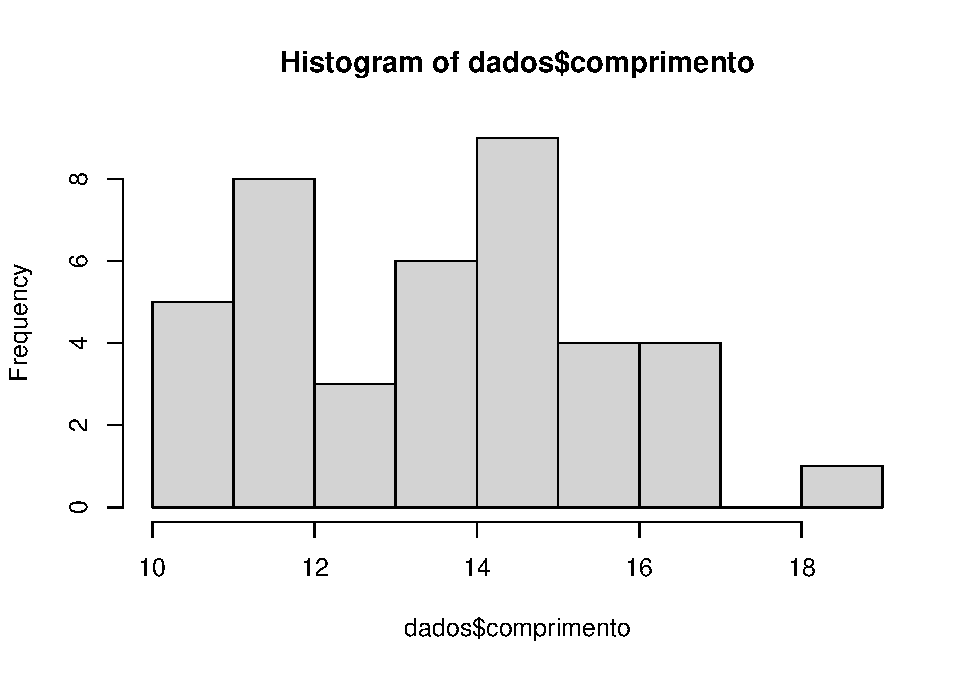
\includegraphics{livroR-1.0_files/figure-latex/comp-hist-1.pdf}
\caption{\label{fig:comp-hist}Comprimento dos organismos da planilha dados}
\end{figure}

Repare que um gráfico foi gerado na sua janela lateral, na guia plots.

Perceba também que voltamos a usar o operador \emph{\$} (cifrão).

Nosso gráfico não está aparentemente muito agradável e um pouco sem cor. Vamos inserir alguns argumentos estéticos que melhoram sua visualização e entender como ele sumariza nossos dados (Figura \ref{fig:comp-hist-col}).

\begin{Shaded}
\begin{Highlighting}[]
\KeywordTok{hist}\NormalTok{(dados}\OperatorTok{$}\NormalTok{comprimento, }
     \DataTypeTok{ylim =} \KeywordTok{c}\NormalTok{(}\DecValTok{0}\NormalTok{, }\DecValTok{10}\NormalTok{), }
     \DataTypeTok{xlim =} \KeywordTok{c}\NormalTok{(}\DecValTok{9}\NormalTok{, }\DecValTok{20}\NormalTok{), }
     \DataTypeTok{col =} \StringTok{"blue"}\NormalTok{,}
     \DataTypeTok{main =} \StringTok{"Meu Histograma"}\NormalTok{,}
     \DataTypeTok{xlab =} \StringTok{"Comprimento"}\NormalTok{,}
     \DataTypeTok{ylab =} \StringTok{"Frequência absoluta"}\NormalTok{)}
\end{Highlighting}
\end{Shaded}

\begin{figure}
\centering
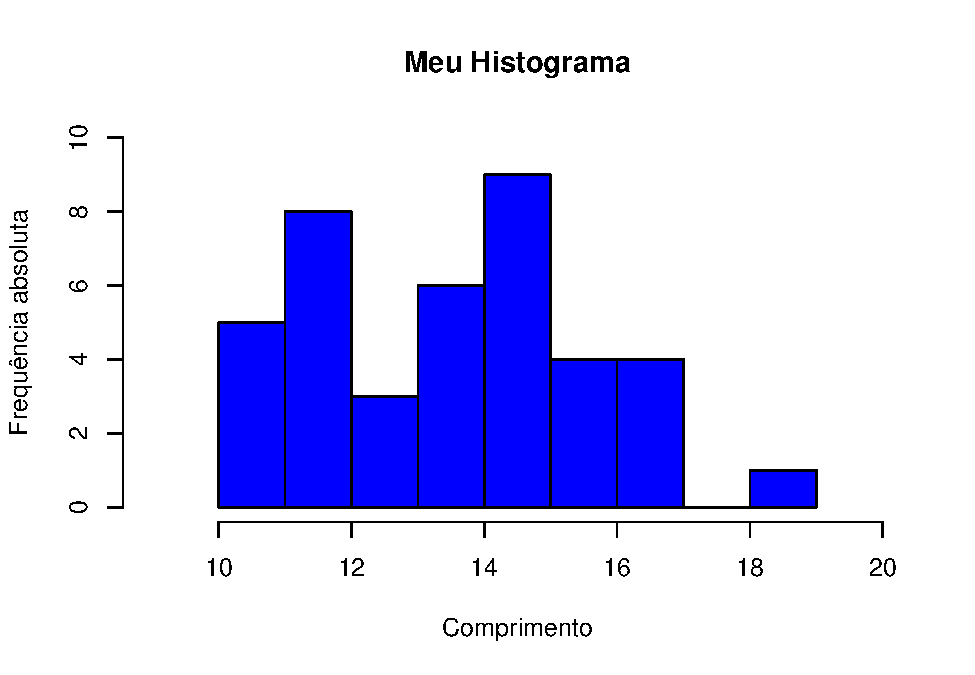
\includegraphics{livroR-1.0_files/figure-latex/comp-hist-col-1.pdf}
\caption{\label{fig:comp-hist-col}Comprimento dos organismos da planilha dados com barras coloridas}
\end{figure}

Temos aqui nosso histograma com alguns argumentos que permitem melhorar sua visualização. Ele nos permite visualizar os dados da variável comprimento e sua frequência de ocorrência.

Podemos observar nele que o valor mínimo observado é 10 e que o máximo é 19 e que as frequências das diferentes classes de comprimento formadas, variam entre 0 e aproximadamente 9. Será que isto que observamos está correto. Vamos ver no tópico a seguir.

Ainda em relação ao histograma podemos ver na função \emph{hist()} que utilizamos diversos argumentos como: xlim, ylim, col, main, xlab e ylab, além de uma função chamada \emph{c()}. Verifique a tabela abaixo para detalhes de cada um desses argumentos e da função \emph{c()}. OBS: Essa função \emph{c()} é muito importante e será utilizada constantemente ao longo de seu trajeto no R.

\textbf{{[}INSERIR TABELA EXPLICANDO OS ARGUMENTOS E A FUNÇÃO CONCATENAR{]}}

\hypertarget{gruxe1fico-de-barras}{%
\subsection{GRÁFICO DE BARRAS}\label{gruxe1fico-de-barras}}

Se já chegamos até esse ponto vamos exercitar um pouco antes de plotar o gráfico de barras.

Acesse a seguinte planilha: abundância. Vamos inseri-la no R com o nome abundancia. repare que retirei o acento. Sempre que trabalharmos com linguagem de programação evite acentuações, espaços, cedilhas (ç) e atente a maiúsculas e minúsculas, pois isso pode interferir no seu código

Se estiver iniciando o R agora lembre-se de definir o ambiente de trabalho.

\begin{Shaded}
\begin{Highlighting}[]
\NormalTok{abundancia <-}\StringTok{ }\KeywordTok{read_excel}\NormalTok{(}\StringTok{"abundancia.xlsx"}\NormalTok{, }\DataTypeTok{col_names =} \OtherTok{TRUE}\NormalTok{)}
\end{Highlighting}
\end{Shaded}

Repare que ela está no formato *.xlsx e apresenta as seguintes variáveis: mes e N. Onde N significa o número de indivíduos observado.

Vamos apenas conferir se está tudo certo com os dados usando a função str().

\begin{Shaded}
\begin{Highlighting}[]
\KeywordTok{str}\NormalTok{(abundancia)}
\end{Highlighting}
\end{Shaded}

\begin{verbatim}
## tibble [12 x 3] (S3: tbl_df/tbl/data.frame)
##  $ mes   : num [1:12] 1 2 3 4 5 6 7 8 9 10 ...
##  $ N     : num [1:12] 100 70 50 30 35 40 60 90 110 150 ...
##  $ desvio: num [1:12] 10 12 11 8 8 14 11 9 12 15 ...
\end{verbatim}

Vamos converter a variável mês em factor.

\begin{Shaded}
\begin{Highlighting}[]
\NormalTok{abundancia}\OperatorTok{$}\NormalTok{mes <-}\StringTok{ }\KeywordTok{as.factor}\NormalTok{(abundancia}\OperatorTok{$}\NormalTok{mes)}
\end{Highlighting}
\end{Shaded}

Repare que agora que sabemos os passos a realizar desde a importação dos arquivos tudo ficou muito mais fácil e fluído, e apenas realizamos três etapas, sendo uma delas apenas conferência.

Seguindo para o gráfico de barras (Figura \ref{fig:bar-abu}) a fim de mostrar o número de indivíduos ao longo dos meses temos que:

\begin{Shaded}
\begin{Highlighting}[]
\KeywordTok{barplot}\NormalTok{(abundancia}\OperatorTok{$}\NormalTok{N)}
\end{Highlighting}
\end{Shaded}

\begin{figure}
\centering
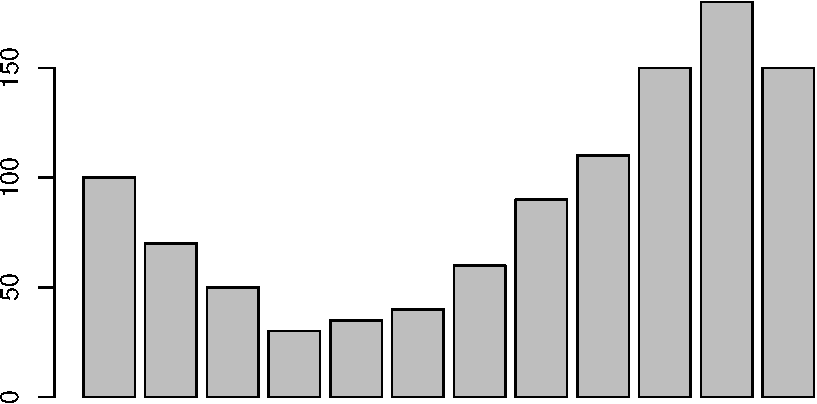
\includegraphics{livroR-1.0_files/figure-latex/bar-abu-1.pdf}
\caption{\label{fig:bar-abu}Gráfico de barras com número de indivíduos da planilha abundância por mês}
\end{figure}

Assim como o histograma o simples uso da função sem argumentos gera um gráfico de dificil análise e esteticamente não muito agradavel.

Vamos portanto adicionar alguns argumentos já conhecidos e outros novos que permitirão a melhor análise do gráfico (Figura \ref{fig:bar-abu-col}).

\begin{Shaded}
\begin{Highlighting}[]
\KeywordTok{barplot}\NormalTok{(abundancia}\OperatorTok{$}\NormalTok{N,}
        \DataTypeTok{ylim =} \KeywordTok{c}\NormalTok{(}\DecValTok{0}\NormalTok{, }\DecValTok{200}\NormalTok{),}
        \DataTypeTok{xlab =} \StringTok{"Mês",}
\StringTok{        ylab = "}\NormalTok{Abundância}\StringTok{",}
\StringTok{        names.arg = abundancia$mes,}
\StringTok{        col = "}\NormalTok{green}\StringTok{")}
\end{Highlighting}
\end{Shaded}

\begin{figure}
\centering
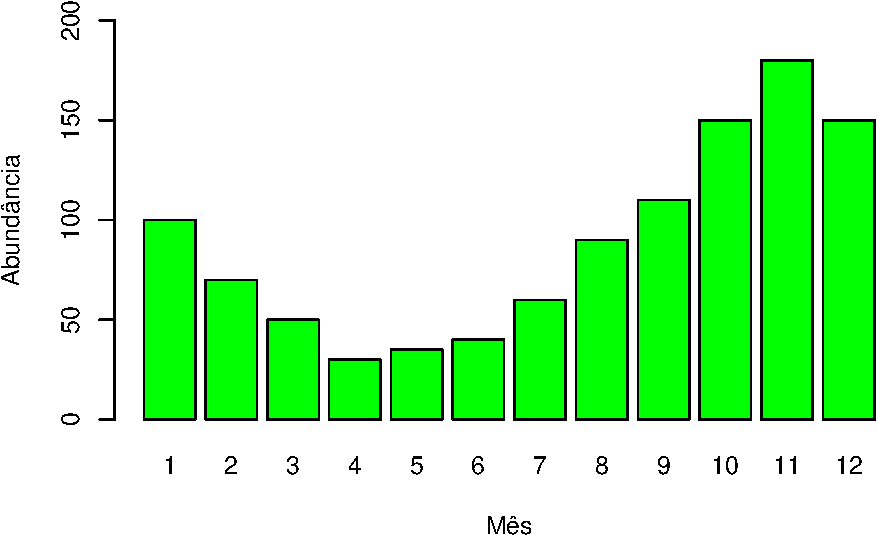
\includegraphics{livroR-1.0_files/figure-latex/bar-abu-col-1.pdf}
\caption{\label{fig:bar-abu-col}Gráfico de barras com número de indivíduos da planilha abundância por mês, com barras coloridas}
\end{figure}

Podemos extrair desse gráfico que a abundância dos indivíduos variam ao longo dos meses com valores mínimos em torno de 50 indivíduos nos meses 4, 5 e 6 e valores máximos em torno de 200 indivíduos no mês 11.

Podemos ver que os argumentos utilizados permitiram referenciar as barras, ajustar o eixo y, adicionar cores e adicionar os nomes dos eixos. Para detalhes sobre os argumentos e funções utilizadas no \emph{barplot()} (Tabela \ref{tab:tab-arg}).

\begin{table}

\caption{\label{tab:tab-arg}Descrição dos argumentos utilizados para o gráfico de barras}
\centering
\begin{tabular}[t]{>{}l>{\raggedright\arraybackslash}p{30em}}
\toprule
Argumentos & Características\\
\midrule
\textbf{\cellcolor{gray!6}{ylim}} & \cellcolor{gray!6}{Refere-se aos limites do eixo y}\\
\textbf{xlab} & É usado para dar nome ao eixo x\\
\textbf{\cellcolor{gray!6}{ylab}} & \cellcolor{gray!6}{É usado para dar nome ao eixo y}\\
\textbf{names.arg} & É usado para definir o nome das categorias/barras representadas no eixo x, neste caso as categorias usadas estão vinculadas a coluna mes do objeto abundancia\\
\textbf{\cellcolor{gray!6}{col}} & \cellcolor{gray!6}{É usado para definir a cor das barras}\\
\bottomrule
\end{tabular}
\end{table}

\textbf{{[}INSERIR TABELA EXPLICANDO OS ARGUMENTOS E A FUNÇÃO CONCATENAR{]}}

\hypertarget{gruxe1fico-de-linhas}{%
\subsection{GRÁFICO DE LINHAS}\label{gruxe1fico-de-linhas}}

Assim como o gráfico de barras podemos desejar fazer um gráfico de linhas para isso podemos utilizar a função \emph{plot()} e continuar trabalhando com os dados de abundância por mês

Contudo para fazer um gráfico de linhas pelo comando básico do R (utilizando a função \emph{plot()}) precisamos indicar que ambos os eixos apresentam variáveis númericas. Portanto teremos que modificar a variável mês de fator para numerica.

Porém não precisamos fazer isso em um comando separado podemos aplicar a função que converte uma variável em númerica dentro da função que plota o gráfico. Vamos visualizar como isso ocorre na prática (Figura \ref{fig:pon-graf}).

\begin{Shaded}
\begin{Highlighting}[]
\KeywordTok{plot}\NormalTok{(}\DataTypeTok{x =} \KeywordTok{as.numeric}\NormalTok{(abundancia}\OperatorTok{$}\NormalTok{mes), }\DataTypeTok{y =}\NormalTok{ abundancia}\OperatorTok{$}\NormalTok{N)}
\end{Highlighting}
\end{Shaded}

\begin{figure}
\centering
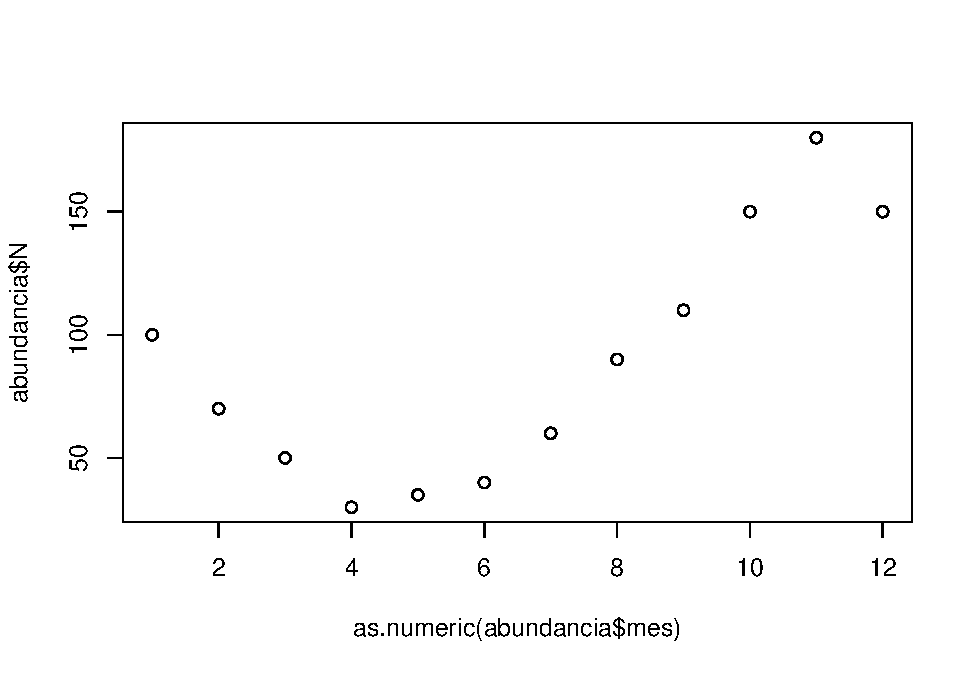
\includegraphics{livroR-1.0_files/figure-latex/pon-graf-1.pdf}
\caption{\label{fig:pon-graf}Representação gráfica do número de indivíduos por mês em pontos}
\end{figure}

Pronto, na função acima aplicamos a função \emph{plot()} indicando os argumentos x e y que definem quem estará no eixo x e quem estará no eixo y, e para a variável que estará no eixo x (variável mês) adicionamos a função \emph{as.numeric()} a qual a converte em númerico apenas para a execução do plot.

Porém a função \emph{plot()} não realizou um gráfico de linhas como esperado, pois para isso precisamos indica-lo por meio de argumentos. Como demonstraremos a seguir (Figura \ref{fig:lin-graf-col}).

\begin{Shaded}
\begin{Highlighting}[]
\KeywordTok{plot}\NormalTok{(}\DataTypeTok{x =} \KeywordTok{as.numeric}\NormalTok{(abundancia}\OperatorTok{$}\NormalTok{mes), }
     \DataTypeTok{y =}\NormalTok{ abundancia}\OperatorTok{$}\NormalTok{N, }
     \DataTypeTok{xlab =} \StringTok{"Mês",}
\StringTok{     ylab = "}\NormalTok{Abundância}\StringTok{",}
\StringTok{     main = "}\NormalTok{Meu gráfico de linha}\StringTok{",}
\StringTok{     ylim = c(0, 200),}
\StringTok{     type = "}\NormalTok{l}\StringTok{",}
\StringTok{     col = "}\NormalTok{green}\StringTok{",}
\StringTok{     lwd = 2)}
\end{Highlighting}
\end{Shaded}

\begin{figure}
\centering
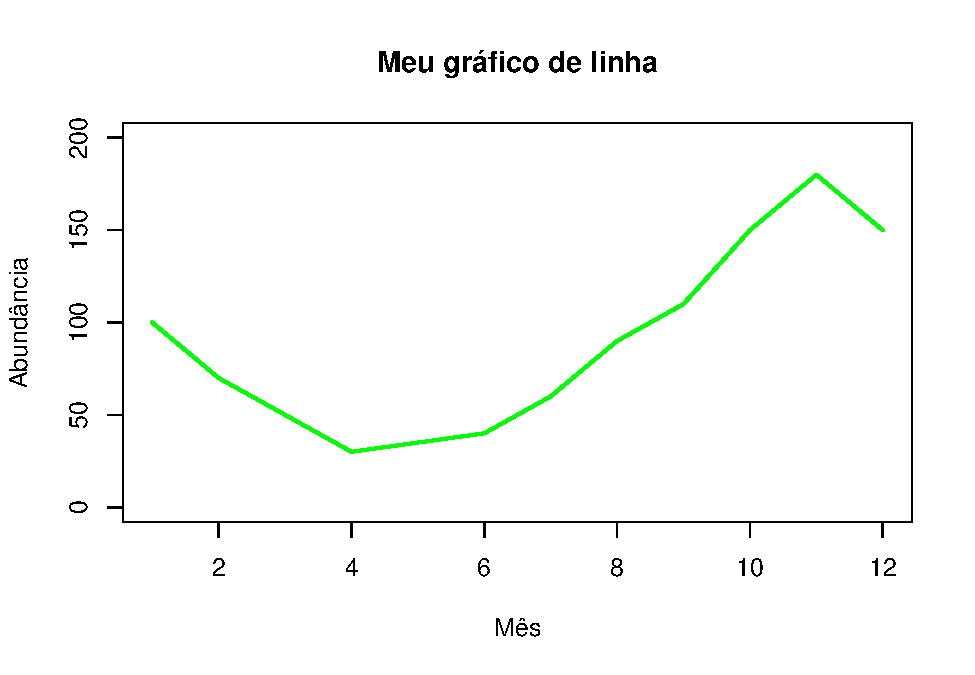
\includegraphics{livroR-1.0_files/figure-latex/lin-graf-col-1.pdf}
\caption{\label{fig:lin-graf-col}Representação gráfica do número de indivíduos por mês em um gráfico de linhas}
\end{figure}

Repare que um gráfico de linha foi plotado e o resultado deste indica o mesmo que o gráfico de barras que realizamos acima.

Alguns argumentos novos foram inseridos, os detalhes deles podem ser visualizados na tabela abaixo:

\textbf{{[}INSERIR TABELA EXPLICANDO OS ARGUMENTOS E A FUNÇÃO CONCATENAR{]}}

\hypertarget{boxplot}{%
\subsection{BOXPLOT}\label{boxplot}}

Vamos voltar a nossa primeira planilha (dados) e executar um gráfico do tipo boxplot (Figura \ref{fig:box-graf}) e ver o que ele nos informa.

\begin{Shaded}
\begin{Highlighting}[]
\KeywordTok{boxplot}\NormalTok{(}\DataTypeTok{formula =}\NormalTok{ dados}\OperatorTok{$}\NormalTok{comprimento }\OperatorTok{~}\StringTok{ }\NormalTok{dados}\OperatorTok{$}\NormalTok{ano)}
\end{Highlighting}
\end{Shaded}

\begin{figure}
\centering
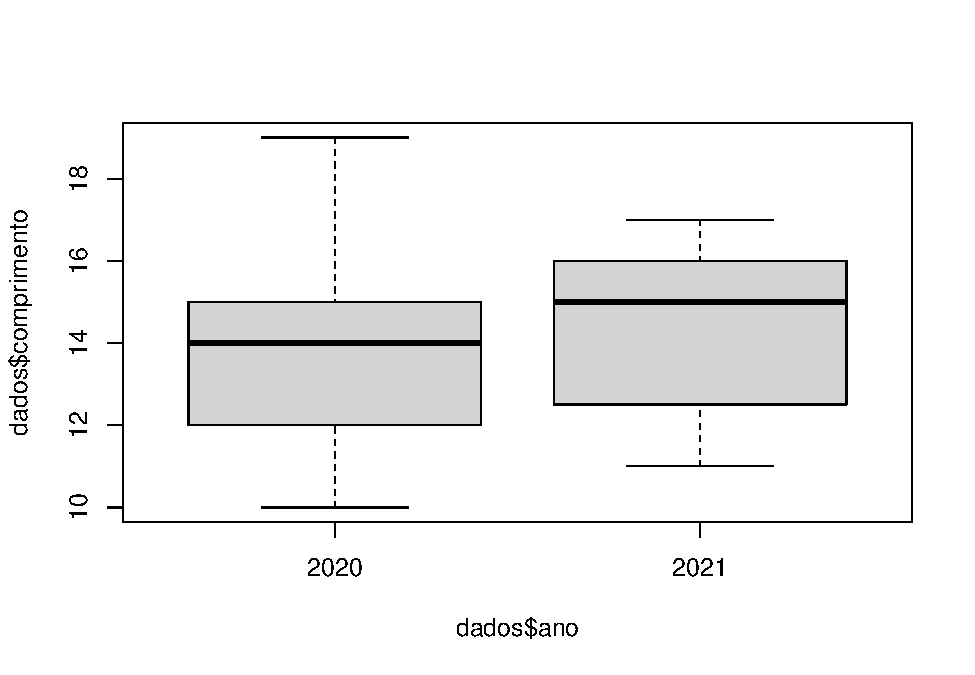
\includegraphics{livroR-1.0_files/figure-latex/box-graf-1.pdf}
\caption{\label{fig:box-graf}Gráfico tipo boxplot do comprimento por ano, da planilha dados}
\end{figure}

Repare que a escrita para esse gráfico é ligeiramente diferente. Ele usa a função \emph{boxplot()}, um argumento chamado formula onde nele inserimos a variável independente (variável do eixo X) e a variável dependente (variável do eixo Y). Entre ambas as variáveis é possível ver o caracter ``\textasciitilde{}'' (til). A forma de ler essa escrita é a seguinte: Realize um boxplot da variável comprimento da planilha dados em função da variável ano da planilha dados. A variável til é lida como (``em função de'')

Vamos adicionar alguns argumentos que permitem deixar o gráfico mais apresentável (Figura \ref{fig:box-graf-col}).

\begin{Shaded}
\begin{Highlighting}[]
\KeywordTok{boxplot}\NormalTok{(}\DataTypeTok{formula =}\NormalTok{ dados}\OperatorTok{$}\NormalTok{comprimento }\OperatorTok{~}\StringTok{ }\NormalTok{dados}\OperatorTok{$}\NormalTok{ano,}
        \DataTypeTok{col =} \KeywordTok{c}\NormalTok{(}\StringTok{"blue"}\NormalTok{, }\StringTok{"green"}\NormalTok{),}
        \DataTypeTok{xlab =} \StringTok{"Ano"}\NormalTok{,}
        \DataTypeTok{ylab =} \StringTok{"Comprimento"}\NormalTok{,}
        \DataTypeTok{main =} \StringTok{"Meu Boxplot"}\NormalTok{)}
\end{Highlighting}
\end{Shaded}

\begin{figure}
\centering
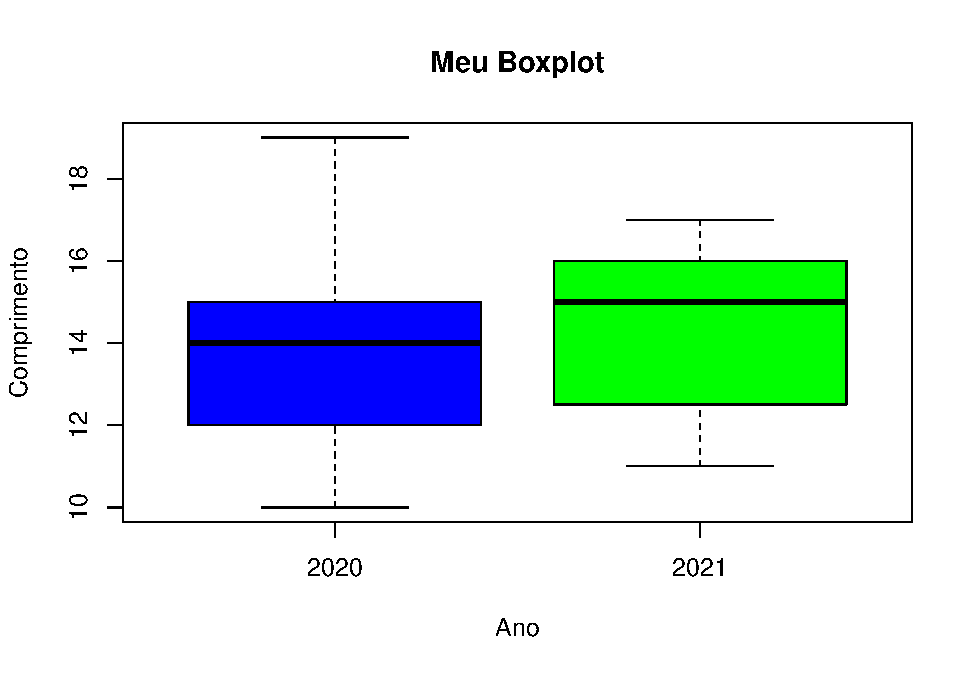
\includegraphics{livroR-1.0_files/figure-latex/box-graf-col-1.pdf}
\caption{\label{fig:box-graf-col}Gráfico tipo boxplot do comprimento por ano com cores por ano, da planilha dados}
\end{figure}

Repare que não adicionamos nenhum argumento ou função diferente do que já fizemos anteriormente. Ou seja, uma vez conhecendo a função, os argumentos por vezes se repetem.

O boxplot porém nos fornece algumas informações extras em relação ao resumo dos dados. Podemos extrair dele dados como média, mediana (segundo quartil), primeiro e terceiro quartil, assim como máximos e mínimos da variável dependente.

As linhas de cada box (caixa) que se referem a cada um dos anos representam, em suas extremidades os valores máximos e mínimos de comprimento de cada ano. A topo e a base de cada ``box'' indicam o primeiro e terceiro quartil, respectivamente, do comprimento. A linha no interior da caixa indica a mediana (segundo quartil) e a metade do box (não indicada graficamente) indica a média.

Podemos por meio desse gráfico então ter uma ideia do que os dados indicam quanto as medidas de tendência central e algumas medidas de dispersão em relação as categorias definidas.

\hypertarget{quarto-passo-sumarizando-os-dados-numericamente}{%
\section{Quarto passo: Sumarizando os dados numericamente}\label{quarto-passo-sumarizando-os-dados-numericamente}}

Temos visto, até este ponto de maneira geral, como resumir os dados graficamente.

Porém muitas vezes precisamos demonstrar numericamente quais são os valores que resumem dos dados. Estes valores consistem nas medidas de tendência central e nas suas medidas de dispersão.

O R permite, de maneira simples, sumarizar os dados por meio da seguinte função.

\begin{Shaded}
\begin{Highlighting}[]
\KeywordTok{summary}\NormalTok{(dados)}
\end{Highlighting}
\end{Shaded}

\begin{verbatim}
##    ano            local     comprimento         peso      
##  2020:20   Ambiente 1:15   Min.   :10.00   Min.   :18.00  
##  2021:20   Ambiente 2:25   1st Qu.:12.00   1st Qu.:20.00  
##                            Median :14.00   Median :21.50  
##                            Mean   :13.97   Mean   :21.73  
##                            3rd Qu.:15.00   3rd Qu.:23.00  
##                            Max.   :19.00   Max.   :28.00
\end{verbatim}

\begin{Shaded}
\begin{Highlighting}[]
\KeywordTok{summary}\NormalTok{(abundancia)}
\end{Highlighting}
\end{Shaded}

\begin{verbatim}
##       mes          N              desvio     
##  1      :1   Min.   : 30.00   Min.   : 8.00  
##  2      :1   1st Qu.: 47.50   1st Qu.: 9.75  
##  3      :1   Median : 80.00   Median :11.50  
##  4      :1   Mean   : 88.75   Mean   :11.75  
##  5      :1   3rd Qu.:120.00   3rd Qu.:14.00  
##  6      :1   Max.   :180.00   Max.   :17.00  
##  (Other):6
\end{verbatim}

Repare que summary(dados) ou summary(abundancia) o R nos informou as variáveis presentes nestas planilhas e quando fator indicou quais são e quantos de cada existem e quando númerico nos retornou valores como média, mediana, mínimo, máximo, primeiro e terceiro quartis.

As medidas de tendência central mais conhecidas e aplicadas são média, mediana e moda.

Para obtenção da média precisamos somar todos os valores e dividir pela quantidade de valores ou no R podemos fazer isso de maneira mais simples por meio da função \emph{mean()}:

\begin{Shaded}
\begin{Highlighting}[]
\KeywordTok{mean}\NormalTok{(dados}\OperatorTok{$}\NormalTok{comprimento)}
\end{Highlighting}
\end{Shaded}

\begin{verbatim}
## [1] 13.975
\end{verbatim}

Como podemos verificar a média do comprimento na planilha dados é de 13.975.

De maneira similar podemos calcular a mediana, que consiste no valor central da distribuição de valores de uma dada variável. Podemos visualiza-la por meio da função \emph{median()}.

\begin{Shaded}
\begin{Highlighting}[]
\KeywordTok{median}\NormalTok{(dados}\OperatorTok{$}\NormalTok{comprimento)}
\end{Highlighting}
\end{Shaded}

\begin{verbatim}
## [1] 14
\end{verbatim}

Como podemos verificar o valor que se encontra no meio da distribuição de valores da variável comprimento é 14.

As medidas de dispersão são utilizadas para demonstrar a variabilidade dos dados\ldots{}{[}explicar mais{]}

Os limites inferior e superior de uma dada variável quantitativa são denominados mínimo e máximo e podem ser obtidos por meio das funções que calculam o mínimo e máximo. Apesar de seu resultado aparecer na função \emph{summary()}, que aplicamos anteriormente, podemos obte-la separadamente para uma variável especifica. Vamos conferi-la com o conjunto de dados que utilizamos anteriormente.

\begin{Shaded}
\begin{Highlighting}[]
\KeywordTok{min}\NormalTok{(dados}\OperatorTok{$}\NormalTok{comprimento)}
\end{Highlighting}
\end{Shaded}

\begin{verbatim}
## [1] 10
\end{verbatim}

\begin{Shaded}
\begin{Highlighting}[]
\KeywordTok{max}\NormalTok{(dados}\OperatorTok{$}\NormalTok{comprimento)}
\end{Highlighting}
\end{Shaded}

\begin{verbatim}
## [1] 19
\end{verbatim}

Uma outra forma de obter os valores máximo e mínimo é usando a função \emph{range()}.

\begin{Shaded}
\begin{Highlighting}[]
\KeywordTok{range}\NormalTok{(dados}\OperatorTok{$}\NormalTok{comprimento)}
\end{Highlighting}
\end{Shaded}

\begin{verbatim}
## [1] 10 19
\end{verbatim}

Como puderam verificar utilizando a função \emph{min()} e \emph{max()} ou \emph{range()} obtemos os valores mínimo e máximo da variável comprimento. Repare que usamos o operador cifrão (\textbf{\$}) após o nome do conjunto de dados. Como você aprendeu anteriormente ele permite acessar as variáveis que estão dentro do objeto dados.

Com os valores mínimo e máximo podemos obter nossa primeira medida de dispersão dos dados. A amplitude que consiste na diferença entre os valores máximo e mínimo de nossa amostra. Está é a forma mais simples de verificar a dispersão de seus dados. Ela apresenta suas falhas, porém tem a vantagem de fornecer a distância na qual seus dados variam na mesma unidade em que eles estão.

A amplitude é utilizada para dados quantitativos, descrever a variabilidade de uma amostra, porém não para inferência estatística.

\begin{Shaded}
\begin{Highlighting}[]
\KeywordTok{max}\NormalTok{(dados}\OperatorTok{$}\NormalTok{comprimento) }\OperatorTok{-}\StringTok{ }\KeywordTok{min}\NormalTok{(dados}\OperatorTok{$}\NormalTok{comprimento)}
\end{Highlighting}
\end{Shaded}

\begin{verbatim}
## [1] 9
\end{verbatim}

Como podemos ver, ao calcular a diferença entre o máximo e mínimo da mesma variável obtemos a diferença entre elas e esse valor consiste na amplitude desta variável.

Uma outra forma de realizar esta mesma operação é utilizando a função \emph{diff()} que calcula a diferença. Quando inserimos a função \emph{range()} dentro da função \emph{diff()} o R nos retorna o resultado da diferença dos valores obtidos pela função \emph{range()}.

\begin{Shaded}
\begin{Highlighting}[]
\KeywordTok{diff}\NormalTok{(}\KeywordTok{range}\NormalTok{(dados}\OperatorTok{$}\NormalTok{comprimento))}
\end{Highlighting}
\end{Shaded}

\begin{verbatim}
## [1] 9
\end{verbatim}

O desvio padrão. Esta é uma das medidas de variação mais importantes que iremos realizar. Ele mede a distância dos valores observados em relação a sua média.

Durante a coleta de dados em estudos ambientais, o que normalmente é extraído de informação é uma fração de um todo, ou seja, uma amostra de uma população. Portanto quando se deseja avaliar o desvio padrão, assim como outras medidas de variabilidade, devemos considerar se estamos avaliando uma amostra ou toda a população. Se uma amostra é considerada o nos referimos a ela como desvio padrão amostral e a representamos por (s) se toda a população é considerada nos referimos a ela como desvio padrão populacional e a representamos por (sigma).

Neste livro vamos abordar e considerar o desvio padrão como o desvio padrão amostral.

Para calcular o desvio padrão amostral utilizamos a seguinte formula abaixo:

\textbf{{[}INSERIR FORMULA{]}}

Podemos calcular o desvio padrão a partir de suas partes, considerando sua formula ou a partir de uma função pré-existente no R. Vamos conferir as duas formas.

Para facilitar o entendimento do código vamos começar criando os seguintes objetos:

\begin{Shaded}
\begin{Highlighting}[]
\NormalTok{comp <-}\StringTok{ }\NormalTok{dados}\OperatorTok{$}\NormalTok{comprimento}
\NormalTok{comp.media <-}\StringTok{ }\KeywordTok{mean}\NormalTok{(dados}\OperatorTok{$}\NormalTok{comprimento)}
\NormalTok{N <-}\StringTok{ }\KeywordTok{length}\NormalTok{(dados}\OperatorTok{$}\NormalTok{comprimento)}

\NormalTok{comp}
\end{Highlighting}
\end{Shaded}

\begin{verbatim}
##  [1] 10 11 15 12 17 14 19 16 15 12 14 15 12 12 14 13 12 11 14 14 13 12 11 15 12
## [26] 14 13 12 11 15 15 17 16 17 15 16 15 16 15 17
\end{verbatim}

\begin{Shaded}
\begin{Highlighting}[]
\NormalTok{comp.media}
\end{Highlighting}
\end{Shaded}

\begin{verbatim}
## [1] 13.975
\end{verbatim}

\begin{Shaded}
\begin{Highlighting}[]
\NormalTok{N}
\end{Highlighting}
\end{Shaded}

\begin{verbatim}
## [1] 40
\end{verbatim}

\begin{itemize}
\tightlist
\item
  ``comp'' contêm os dados da variável comprimento presente na planilha dados
\item
  ``comp.media'' contêm um dado que consiste na média da variável comprimento
\item
  ``N'' representa a quantidade de observações presentes na variável comprimento. Repare que aqui utilizamos uma nova função chamada length() a qual contabiliza o número de observações de objeto.
\end{itemize}

\begin{Shaded}
\begin{Highlighting}[]
\KeywordTok{sqrt}\NormalTok{((}\KeywordTok{sum}\NormalTok{((comp }\OperatorTok{-}\StringTok{ }\NormalTok{comp.media)}\OperatorTok{^}\DecValTok{2}\NormalTok{)) }\OperatorTok{/}\StringTok{ }\NormalTok{(N }\OperatorTok{-}\StringTok{ }\DecValTok{1}\NormalTok{))}
\end{Highlighting}
\end{Shaded}

\begin{verbatim}
## [1] 2.106005
\end{verbatim}

\begin{Shaded}
\begin{Highlighting}[]
\KeywordTok{sd}\NormalTok{(dados}\OperatorTok{$}\NormalTok{comprimento)}
\end{Highlighting}
\end{Shaded}

\begin{verbatim}
## [1] 2.106005
\end{verbatim}

\begin{Shaded}
\begin{Highlighting}[]
\KeywordTok{sd}\NormalTok{(comp)}
\end{Highlighting}
\end{Shaded}

\begin{verbatim}
## [1] 2.106005
\end{verbatim}

Destas três formas cabe explicarmos a primeira. Nela vamos entender como lemos uma função. O ideal é ler de dentro para fora. Como uma equação matemática. Mas não se assuste é mais fácil do que parece. Começamos a leitura da seguinte forma:

\begin{enumerate}
\def\labelenumi{\arabic{enumi}.}
\tightlist
\item
  (comp - comp.media): Realize a diferença dos valores presentes em comp de sua média.
\item
  ((comp - comp.media)\^{}2): Eleve esses valores, obtidos da diferença, ao quadrado.
\item
  (sum((comp - comp.media)\^{}2)): Soma todos os valores, obtidos pela diferença elevados ao quadrado.
\item
  (sum((comp - comp.media)\^{}2)) / (N - 1): Divida a soma dos valores da diferença elevado ao quadrado pelo número de observações menos 1.
\item
  sqrt((sum((comp - comp.media)\^{}2)) / (N - 1)): Extraia a raíz quadrada da divisão da soma dos valores da diferença elevado ao quadrado pelo número de observações menos 1.
\end{enumerate}

Repare que a leitura segue a ordem dos passos do cálculo que seria feito a mão usando a equação apresentada acima.

Mas caso não queira escrever a formula o R fornece a função \emph{sd()} que pode ser aplicada a uma variável dentro de uma planilha de dados ou a um vetor que contenha um conjunto de observações do seu interesse.

Pronto, agora enetendemos como ler um código que apresenta funções dentro de funções e entendemos como realizar o desvio padrão de três formas distintas (existem diversas outras formas) no R. Agora você já pode escolher a que mais lhe agrada. Qual você prefere? Bem, essa é uma escolha sua.

Assim como o desvio padrão temos também a variância. A mais importante medida de variabilidade dos dados. Há todo um conjunto espécial de análise de dados voltado para ela. Mas como poderão ver, ela não difere muito do desvio padrão, apenas pelo fato de que consiste no seu valor elevado ao quadrado, no entanto a variância amostral é representada por s² enquanto que o desvio padrão é representado por s.

Partindo dessa ideia a variância é nada mais que estimar o desvio padrão e eleva-lo ao quadrado. Vamos observar o seu resultado utilizando sua formula e a função predefinida pelo R.

\begin{Shaded}
\begin{Highlighting}[]
\NormalTok{(}\KeywordTok{sum}\NormalTok{((comp }\OperatorTok{-}\StringTok{ }\NormalTok{comp.media)}\OperatorTok{^}\DecValTok{2}\NormalTok{)) }\OperatorTok{/}\StringTok{ }\NormalTok{(N }\OperatorTok{-}\StringTok{ }\DecValTok{1}\NormalTok{)}
\end{Highlighting}
\end{Shaded}

\begin{verbatim}
## [1] 4.435256
\end{verbatim}

\begin{Shaded}
\begin{Highlighting}[]
\KeywordTok{sd}\NormalTok{(dados}\OperatorTok{$}\NormalTok{comprimento)}\OperatorTok{^}\DecValTok{2}
\end{Highlighting}
\end{Shaded}

\begin{verbatim}
## [1] 4.435256
\end{verbatim}

\begin{Shaded}
\begin{Highlighting}[]
\KeywordTok{var}\NormalTok{(dados}\OperatorTok{$}\NormalTok{comprimento)}
\end{Highlighting}
\end{Shaded}

\begin{verbatim}
## [1] 4.435256
\end{verbatim}

Pronto aqui estão 3 maneiras de encontrar a variância de seus dados. A primeira é similar ao que realizamos anteriormente para o desvio padrão porém sem a raíz quadrada. A segunda consiste em elevar ao quadrado o resultado do desvio padrão e a terceira é aplicando a função \emph{var()} a variável comprimento presente na planilha dados.

Difícil? Espero que não.

Mas vamos entender o significado do desvio padrão e variância. Pois ambos estão intimamente relacionados.

Como conversamos anteriormente as medidas de tendência central nos informam sobre a distância das observações de uma dada variável em relação a sua medida de tendência central (normalmente a média). Se somarmos a diferença das observações de uma dada variável de sua média obteremos o valor de 0 (tabela abaixo). Contudo se elevarmos cada diferença ao quadrado e dividirmos pela quantidade de observações menos 1 (subtrai-se 1 das observações porque estamos trabalhando com amostras) teremos a média das distâncias das observações ao quadrado (variância). Porém algumas vezes esse valor pode não ser fácil de interpretar e não reflete diretamente a unidade da variável mensurada. Com isso uma forma mais intuitiva utilizada para interpretar a dispersão dos dados em relação a sua média consiste no desvio padrão, pois como vimos este consiste na raiz quadrada da variância, ao fazermos isso nos obtemos a distância média das observações em relação a sua média na mesma unidade de medida em que se encontram.

O coeficiente de variação é outra medida importante e de fácil interpretação sobre a variabilidade dos dados. Este consiste em representar o desvio padrão em termos percentuais. Este é simples de calcular e intuitivo de interpretar.

Não há, até o momento, uma função no pacote básico do R que o calcule. Vamos calcular e ver o que ele quer dizer.

\begin{Shaded}
\begin{Highlighting}[]
\KeywordTok{sd}\NormalTok{(dados}\OperatorTok{$}\NormalTok{comprimento)}\OperatorTok{/}\KeywordTok{mean}\NormalTok{(dados}\OperatorTok{$}\NormalTok{comprimento)}\OperatorTok{*}\DecValTok{100}
\end{Highlighting}
\end{Shaded}

\begin{verbatim}
## [1] 15.0698
\end{verbatim}

Pronto, calculamos o coeficiente de variação da variável comprimento. O desvio padrão de uma dada observação apresenta a mesma unidade de suas observações, correto? Então podemos dividi-lo pela média das próprias observações e multiplicar por 100 com isso temos que a variável comprimento tem uma variação em torno da média de ±15,07\%.

Com isso verificamos as principais medidas de tendência central e dispersão. Mas fica uma questão, como incorpora-las aos gráficos para que assim possamos resumir os dados graficamente de maneira mais completa.

Vamos em frente! Vamos utilizar nossa planilha dados e verificar a média do comprimento e do peso por ano e por ambiente e incorporar em cada um dos gráficos seus respectivos desvios padrões.

Neste caso vamos primeiro precisar organizar os dados que queremos plotar. Como desejamos plotar a média do comprimento por ano e ambiente, vamos primeiro construir passo a passo uma tabela que apresente 4 colunas a primeira com o ano, a segunda com ambiente, a terceira com a média do comprimento e a última com o desvio padrão.

\begin{Shaded}
\begin{Highlighting}[]
\NormalTok{dados}\FloatTok{.2}\NormalTok{ <-}\StringTok{ }\KeywordTok{split}\NormalTok{(}\DataTypeTok{x =}\NormalTok{ dados, }\DataTypeTok{f =}\NormalTok{ dados}\OperatorTok{$}\NormalTok{ano)}

\NormalTok{ano}\FloatTok{.2020}\NormalTok{ <-}\StringTok{ }\NormalTok{dados}\FloatTok{.2}\OperatorTok{$}\StringTok{`}\DataTypeTok{2020}\StringTok{`}
\NormalTok{ano}\FloatTok{.2021}\NormalTok{ <-}\StringTok{ }\NormalTok{dados}\FloatTok{.2}\OperatorTok{$}\StringTok{`}\DataTypeTok{2021}\StringTok{`}

\NormalTok{ano.}\FloatTok{2020.}\NormalTok{local <-}\StringTok{ }\KeywordTok{split}\NormalTok{(}\DataTypeTok{x =}\NormalTok{ ano}\FloatTok{.2020}\NormalTok{, }\DataTypeTok{f =}\NormalTok{ ano}\FloatTok{.2020}\OperatorTok{$}\NormalTok{local)}
\NormalTok{ano.}\FloatTok{2021.}\NormalTok{local <-}\StringTok{ }\KeywordTok{split}\NormalTok{(}\DataTypeTok{x =}\NormalTok{ ano}\FloatTok{.2021}\NormalTok{, }\DataTypeTok{f =}\NormalTok{ ano}\FloatTok{.2021}\OperatorTok{$}\NormalTok{local)}

\NormalTok{ano.}\FloatTok{2020.}\NormalTok{local}\FloatTok{.1}\NormalTok{ <-}\StringTok{ }\NormalTok{ano.}\FloatTok{2020.}\NormalTok{local}\OperatorTok{$}\StringTok{`}\DataTypeTok{Ambiente 1}\StringTok{`}
\NormalTok{ano.}\FloatTok{2020.}\NormalTok{local}\FloatTok{.2}\NormalTok{ <-}\StringTok{ }\NormalTok{ano.}\FloatTok{2020.}\NormalTok{local}\OperatorTok{$}\StringTok{`}\DataTypeTok{Ambiente 2}\StringTok{`}

\NormalTok{ano.}\FloatTok{2021.}\NormalTok{local}\FloatTok{.1}\NormalTok{ <-}\StringTok{ }\NormalTok{ano.}\FloatTok{2021.}\NormalTok{local}\OperatorTok{$}\StringTok{`}\DataTypeTok{Ambiente 1}\StringTok{`}
\NormalTok{ano.}\FloatTok{2021.}\NormalTok{local}\FloatTok{.2}\NormalTok{ <-}\StringTok{ }\NormalTok{ano.}\FloatTok{2021.}\NormalTok{local}\OperatorTok{$}\StringTok{`}\DataTypeTok{Ambiente 2}\StringTok{`}
\end{Highlighting}
\end{Shaded}

Pronto! Dividimos os nosso dados de acordo com os fatores que desejamos. Agora vamos obter as métricas média e desvio padrão.

\begin{Shaded}
\begin{Highlighting}[]
\NormalTok{ano.}\FloatTok{2020.}\NormalTok{local.}\FloatTok{1.}\NormalTok{comp.media <-}\StringTok{ }\KeywordTok{mean}\NormalTok{(ano.}\FloatTok{2020.}\NormalTok{local}\FloatTok{.1}\OperatorTok{$}\NormalTok{comprimento)}
\NormalTok{ano.}\FloatTok{2020.}\NormalTok{local.}\FloatTok{1.}\NormalTok{comp.dp <-}\StringTok{ }\KeywordTok{sd}\NormalTok{(ano.}\FloatTok{2020.}\NormalTok{local}\FloatTok{.1}\OperatorTok{$}\NormalTok{comprimento)}

\NormalTok{ano.}\FloatTok{2020.}\NormalTok{local.}\FloatTok{2.}\NormalTok{comp.media <-}\StringTok{ }\KeywordTok{mean}\NormalTok{(ano.}\FloatTok{2020.}\NormalTok{local}\FloatTok{.2}\OperatorTok{$}\NormalTok{comprimento)}
\NormalTok{ano.}\FloatTok{2020.}\NormalTok{local.}\FloatTok{2.}\NormalTok{comp.dp <-}\StringTok{ }\KeywordTok{sd}\NormalTok{(ano.}\FloatTok{2020.}\NormalTok{local}\FloatTok{.2}\OperatorTok{$}\NormalTok{comprimento)}

\NormalTok{ano.}\FloatTok{2021.}\NormalTok{local.}\FloatTok{1.}\NormalTok{comp.media <-}\StringTok{ }\KeywordTok{mean}\NormalTok{(ano.}\FloatTok{2021.}\NormalTok{local}\FloatTok{.1}\OperatorTok{$}\NormalTok{comprimento)}
\NormalTok{ano.}\FloatTok{2021.}\NormalTok{local.}\FloatTok{1.}\NormalTok{comp.dp <-}\StringTok{ }\KeywordTok{sd}\NormalTok{(ano.}\FloatTok{2021.}\NormalTok{local}\FloatTok{.1}\OperatorTok{$}\NormalTok{comprimento)}

\NormalTok{ano.}\FloatTok{2021.}\NormalTok{local.}\FloatTok{2.}\NormalTok{comp.media <-}\StringTok{ }\KeywordTok{mean}\NormalTok{(ano.}\FloatTok{2021.}\NormalTok{local}\FloatTok{.2}\OperatorTok{$}\NormalTok{comprimento)}
\NormalTok{ano.}\FloatTok{2021.}\NormalTok{local.}\FloatTok{2.}\NormalTok{comp.dp <-}\StringTok{ }\KeywordTok{sd}\NormalTok{(ano.}\FloatTok{2021.}\NormalTok{local}\FloatTok{.2}\OperatorTok{$}\NormalTok{comprimento)}
\end{Highlighting}
\end{Shaded}

Pronto! Média e desvio padrão do comprimento calculado para cada ano e local. Agora vamos unir esses resultados em uma data frame

\begin{Shaded}
\begin{Highlighting}[]
\NormalTok{dados.media <-}\StringTok{ }\KeywordTok{c}\NormalTok{(ano.}\FloatTok{2020.}\NormalTok{local.}\FloatTok{1.}\NormalTok{comp.media,}
\NormalTok{                 ano.}\FloatTok{2020.}\NormalTok{local.}\FloatTok{2.}\NormalTok{comp.media,}
\NormalTok{                 ano.}\FloatTok{2021.}\NormalTok{local.}\FloatTok{1.}\NormalTok{comp.media,}
\NormalTok{                 ano.}\FloatTok{2021.}\NormalTok{local.}\FloatTok{2.}\NormalTok{comp.media)}

\NormalTok{dados.dp <-}\StringTok{ }\KeywordTok{c}\NormalTok{(ano.}\FloatTok{2020.}\NormalTok{local.}\FloatTok{1.}\NormalTok{comp.dp,}
\NormalTok{              ano.}\FloatTok{2020.}\NormalTok{local.}\FloatTok{2.}\NormalTok{comp.dp,}
\NormalTok{              ano.}\FloatTok{2021.}\NormalTok{local.}\FloatTok{1.}\NormalTok{comp.dp,}
\NormalTok{              ano.}\FloatTok{2021.}\NormalTok{local.}\FloatTok{2.}\NormalTok{comp.dp)}
\end{Highlighting}
\end{Shaded}

Vamos criar as variáveis categoricas e ano e local para adicionar a esse dados

\begin{Shaded}
\begin{Highlighting}[]
\NormalTok{ano <-}\StringTok{ }\KeywordTok{c}\NormalTok{(}\StringTok{"2020"}\NormalTok{, }\StringTok{"2020"}\NormalTok{, }\StringTok{"2021"}\NormalTok{, }\StringTok{"2021"}\NormalTok{)}
\NormalTok{local <-}\StringTok{ }\KeywordTok{c}\NormalTok{(}\StringTok{"Ambiente 1"}\NormalTok{, }\StringTok{"Ambiente 2"}\NormalTok{, }\StringTok{"Ambiente 1"}\NormalTok{, }\StringTok{"Ambiente 2"}\NormalTok{)}

\NormalTok{dados}\FloatTok{.3}\NormalTok{ <-}\StringTok{ }\KeywordTok{as.data.frame}\NormalTok{(}\KeywordTok{cbind}\NormalTok{(ano, local, dados.media, dados.dp))}
\KeywordTok{str}\NormalTok{(dados}\FloatTok{.3}\NormalTok{)}
\end{Highlighting}
\end{Shaded}

\begin{verbatim}
## 'data.frame':    4 obs. of  4 variables:
##  $ ano        : chr  "2020" "2020" "2021" "2021"
##  $ local      : chr  "Ambiente 1" "Ambiente 2" "Ambiente 1" "Ambiente 2"
##  $ dados.media: chr  "14.1" "13.1" "13" "14.8"
##  $ dados.dp   : chr  "2.84604989415154" "1.28668393770792" "1.58113883008419" "1.93464651625488"
\end{verbatim}

\begin{Shaded}
\begin{Highlighting}[]
\NormalTok{dados}\FloatTok{.3}\OperatorTok{$}\NormalTok{ano <-}\StringTok{ }\KeywordTok{as.factor}\NormalTok{(dados}\FloatTok{.3}\OperatorTok{$}\NormalTok{ano)}
\NormalTok{dados}\FloatTok{.3}\OperatorTok{$}\NormalTok{local <-}\StringTok{ }\KeywordTok{as.factor}\NormalTok{(dados}\FloatTok{.3}\OperatorTok{$}\NormalTok{local)}
\NormalTok{dados}\FloatTok{.3}\OperatorTok{$}\NormalTok{dados.media <-}\StringTok{ }\KeywordTok{as.numeric}\NormalTok{(dados}\FloatTok{.3}\OperatorTok{$}\NormalTok{dados.media)}
\NormalTok{dados}\FloatTok{.3}\OperatorTok{$}\NormalTok{dados.dp <-}\StringTok{ }\KeywordTok{as.numeric}\NormalTok{(dados}\FloatTok{.3}\OperatorTok{$}\NormalTok{dados.dp)}
\end{Highlighting}
\end{Shaded}

\begin{Shaded}
\begin{Highlighting}[]
\NormalTok{dados}\FloatTok{.3}
\end{Highlighting}
\end{Shaded}

\begin{verbatim}
##    ano      local dados.media dados.dp
## 1 2020 Ambiente 1        14.1 2.846050
## 2 2020 Ambiente 2        13.1 1.286684
## 3 2021 Ambiente 1        13.0 1.581139
## 4 2021 Ambiente 2        14.8 1.934647
\end{verbatim}

Repare que durante todo este processo utilizamos três funções que não haviamos utilizado antes. As funções \emph{split()} que divide a planilha de acordo com as categorias presentes na variável que definimos, \emph{as.data.frame()} que faz com que um conjunto de objetos sejam convertidos em data frame e \emph{cbind()} o qual une objetos como colunas. Essas funções também serão comumente utilizadas durante seus passos iniciais no R.

Pronto! depois de alguns passos conseguimos construir nossa nova tabela com os dados resumidos.

É um processo longo porém necessário para se acostumar com o ambiente de trabalho e a linguagem que o R usa. Há caminhos mais rápidos e tão eficientes quanto. Que se tornam uteis quando lidamos com muitas categorias dentro de uma variável. Contudo para isso é necessário a instalação de algum pacote (Há vários pacotes que apresentam funções que realizam este processo). Vamos utilizar um exemplo começando pela instalação do pacote chamado Rmisc.

O comando abaixo realiza a instalação desse pacote. Conforme já fizemos com o pacote readxl

\begin{Shaded}
\begin{Highlighting}[]
\CommentTok{## install.packages("Rmisc")}
\end{Highlighting}
\end{Shaded}

Após instalado vamos carrega-lo pelo comando a seguir. Conforme já fizemos com o pacote readxl

\begin{Shaded}
\begin{Highlighting}[]
\KeywordTok{library}\NormalTok{(Rmisc)}
\end{Highlighting}
\end{Shaded}

Agora vamos conhecer a função \emph{summarySE()} deste pacote o qual realiza os passos que fizemos acima e ainda apresenta outros resultados. Mas iremos focar na média e desvio padrão.

\begin{Shaded}
\begin{Highlighting}[]
\NormalTok{resultado <-}\StringTok{ }\KeywordTok{summarySE}\NormalTok{(}\DataTypeTok{data =}\NormalTok{ dados, }
                       \DataTypeTok{measurevar =} \StringTok{"comprimento"}\NormalTok{, }
                       \DataTypeTok{groupvars =} \KeywordTok{c}\NormalTok{(}\StringTok{"ano"}\NormalTok{, }\StringTok{"local"}\NormalTok{))}

\NormalTok{resultado}
\end{Highlighting}
\end{Shaded}

\begin{verbatim}
##    ano      local  N comprimento       sd        se        ci
## 1 2020 Ambiente 1 10        14.1 2.846050 0.9000000 2.0359414
## 2 2020 Ambiente 2 10        13.1 1.286684 0.4068852 0.9204382
## 3 2021 Ambiente 1  5        13.0 1.581139 0.7071068 1.9632432
## 4 2021 Ambiente 2 15        14.8 1.934647 0.4995236 1.0713715
\end{verbatim}

Repare que a função \emph{summarySE()} apresenta, basicamente, 3 argumentos, ``data'' que pede que se insira a planilha a ser utilizada, ``measurevar'' o qual pede a variável quantitativa que será sumarizada e ``groupvars'' o qual pede as variáveis categoricas segundo as quais a variável mensurável será agrupada. Observe também que para esta função as variáveis devem ser colocadas entre aspas.

Pronto com a função acima realizamos os mesmos passos que antes e guardamos o resultado dentro de um objeto chamado resultado. Repare que essa função nos resumiu os dados de comprimento de acordo com as duas variáveis categóricas que indicamos: ano e local. Em seu resumo ele nos forneceu, na seguinte ordem, a coluna ano, local, N (número de observações), comprimento (média do comprimento), sd (desvio padrão), se (erro padrão), ci (intervalo de confiança de 95\%).

Agora vamos usar o objeto resultado para desenvolver o gráfico de barras com o erro padrão (Figura \ref{fig:bar-ep}). Mas lembre-se o objeto dados.3 também pode ser utilizado.

\begin{Shaded}
\begin{Highlighting}[]
\NormalTok{grafico <-}\StringTok{ }\KeywordTok{barplot}\NormalTok{(}\DataTypeTok{formula =}\NormalTok{ comprimento }\OperatorTok{~}\StringTok{ }\NormalTok{ano }\OperatorTok{+}\StringTok{ }\NormalTok{local,}
                   \DataTypeTok{data =}\NormalTok{ resultado,}
                   \DataTypeTok{beside =} \OtherTok{TRUE}\NormalTok{,}
                   \DataTypeTok{col =} \KeywordTok{c}\NormalTok{(}\StringTok{"red"}\NormalTok{, }\StringTok{"blue"}\NormalTok{),}
                   \DataTypeTok{ylim =} \KeywordTok{c}\NormalTok{(}\DecValTok{0}\NormalTok{, }\DecValTok{30}\NormalTok{),}
                   \DataTypeTok{ylab =} \StringTok{"Comprimento médio (cm)"}\NormalTok{,}
                   \DataTypeTok{legend.text =} \OtherTok{TRUE}\NormalTok{)}

\KeywordTok{arrows}\NormalTok{(}\DataTypeTok{x0 =}\NormalTok{ grafico,}
       \DataTypeTok{y0 =}\NormalTok{ resultado}\OperatorTok{$}\NormalTok{comprimento }\OperatorTok{+}\StringTok{ }\NormalTok{resultado}\OperatorTok{$}\NormalTok{sd,}
       \DataTypeTok{y1 =}\NormalTok{ resultado}\OperatorTok{$}\NormalTok{comprimento }\OperatorTok{-}\StringTok{ }\NormalTok{resultado}\OperatorTok{$}\NormalTok{sd,}
       \DataTypeTok{code =} \DecValTok{3}\NormalTok{,}
       \DataTypeTok{angle =} \DecValTok{90}\NormalTok{,}
       \DataTypeTok{length =} \FloatTok{0.05}\NormalTok{)}
\end{Highlighting}
\end{Shaded}

\begin{figure}
\centering
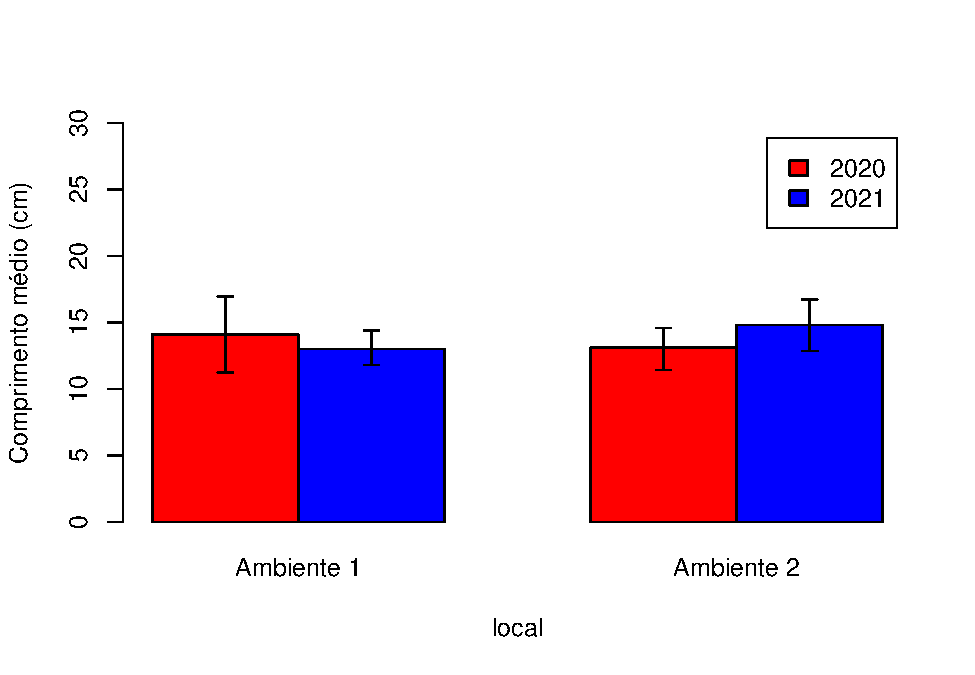
\includegraphics{livroR-1.0_files/figure-latex/bar-ep-1.pdf}
\caption{\label{fig:bar-ep}Gráfico de barras com erro padrão do comprimento por ano e local, da planilha resultado (derivada da planilha dados)}
\end{figure}

Note que nesta função \emph{barplot()} utilizamos algumas mudanças em relação ao que fizemos anteriormente, como os argumentos ``formula'' o qual indica a variável resposta em função das variáveis categóricas o qual será plotado (Caso altere a ordem ano + local para local + ano a ordem do gráfico também será alterado. Teste você mesmo, veja o acontece). Neste caso como temos mais de uma variável categórica adicionamos um argumento novo chamado ``legend.text'' o qual adiciona uma legenda ao gráfico.

Para adicionar os desvios no gráfico de barras precisamos criar um objeto que armazena o gráfico, por isso adicionamos a função barplot() a um objeto denominado grafico.

Agora que construimos o gráfico, a função \emph{arrows()} é responsável por adicionar as barras de desvios no gráfico. Ela apresenta alguns argumentos diferentes do que já vimos em outros gráficos. ``x0'' indica o objeto onde o gráfico foi armazenado; ``y0'' e ``y1'' são escritos como uma operação matemática onde devemos incluir o valor da média + e - a coluna onde está a variável referente ao desvio; ``code'' determina o tipo de seta que será plotada; ``angle'' é o ângulo da haste da barra até a ponta; ``length'' é o comprimento das bordas da barra.

Terminamos de construir e entender os componentes do nosso primeiro gráfico com suas barras de erro.

O entendimento principal para construção desse gráfico consiste em entender como organizar os dados a serem graficados. Ao se usar a função \emph{barplot()} para construção do gráfico de barras com os desvios, devemos ter uma ou mais colunas com as categorias, outra com os valores que desejamos e outra com os valores dos desvios.

Vamos realizar um segundo tipo de gráfico onde temos apenas uma variável categórica e seus respectivos desvios. Para isso utilizaremos nosso conjunto de dados abundancia (lembre-se que mês é uma variável categórica e deve ser identificada como fator) (Figura @ref(fig(bar-ep-abu))).

Neste conjunto de dados não precisamos reorganizar os dados pois eles já se encontram organizados e já temos os valores dos desvios.

\begin{Shaded}
\begin{Highlighting}[]
\NormalTok{grafico <-}\StringTok{ }\KeywordTok{barplot}\NormalTok{(abundancia}\OperatorTok{$}\NormalTok{N,}
                   \DataTypeTok{ylim =} \KeywordTok{c}\NormalTok{(}\DecValTok{0}\NormalTok{, }\DecValTok{200}\NormalTok{),}
                   \DataTypeTok{xlab =} \StringTok{"Mês",}
\StringTok{                   ylab = "}\NormalTok{Abundância}\StringTok{",}
\StringTok{                   names.arg = abundancia$mes,}
\StringTok{                   col = "}\NormalTok{green}\StringTok{")}

\StringTok{arrows(x0 = grafico,}
\StringTok{       y0 = abundancia$N + abundancia$desvio,}
\StringTok{       y1 = abundancia$N - abundancia$desvio,}
\StringTok{       code = 3,}
\StringTok{       angle = 90,}
\StringTok{       length = 0.05)}
\end{Highlighting}
\end{Shaded}

\begin{figure}
\centering
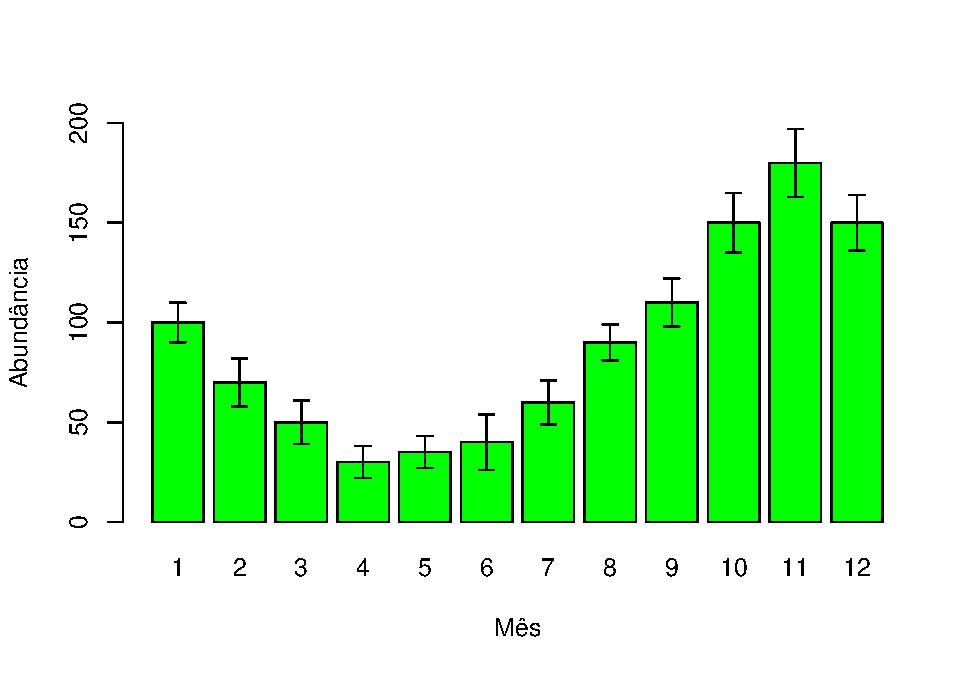
\includegraphics{livroR-1.0_files/figure-latex/bar-ep-abu-1.pdf}
\caption{\label{fig:bar-ep-abu}Gráfico de barras com erro padrão da abundância por mês da planilha abundância}
\end{figure}

Repare que é quase a mesma coisa que fizemos antes. A única diferença é que guardamos o gráfico gerado em um objeto chamado grafico.

Pronto, gráfico realizado.

Durante nosso percurso neste livro realizaremos muito mais gráficos aliados as análises estatísticas básicas mais comumente utilizadas. Não se assuste com a quantidade de etapas e funções e argumentos e nomes, eles irão se repetir tantas e tantas vezes daqui em diante que você não esquecerá. O aprendizado do R é exponencial e ele lhe permitirá entender como nunca o mundo da análise de dados.

\textbf{Resumo das etapas até o presente momento:}
\textbf{importar planinha \textgreater{}\textgreater{} conferir as variáveis \textgreater{}\textgreater{} sumarizar numericamente os dados \textgreater{}\textgreater{} sumarizar graficamente os dados}

\textbf{{[}TEMOS QUE FAZER UM ESQUEMA DESSAS ETAPAS{]}}

\hypertarget{qui-quadrado-ux3c7}{%
\chapter{Qui-quadrado (χ²)}\label{qui-quadrado-ux3c7}}

Em alguns momentos podemos estar trabalhando com variáveis categóricas e lidarmos com perguntas sobre estas variáveis e portanto pode ser necessário avaliarmos se a frequência das observações de uma dada variável categórica se ajusta ao que se é esperado (χ² para ajuste de frequências) ou se as proporções das observações de duas ou mais variáveis categóricas são independentes uma da outra (χ² para independência).

Portanto, como podemos perceber, para este teste iremos precisar apenas de uma variável (se estivermos avaliando o ajuste de frequências) ou duas variáveis (se avaliarmos a independência) e estas devem ser categóricas. Como aprendemos anteriormente as variáveis categóricas devem ser classificadas como factor (pela função \emph{as.factor()}) no R.

Vamos conferir em detalhes e com exemplos como realizar estas duas análises no R. Mas antes vamos sumarizar suas principais características.

\textbf{{[}FAZER UMA TABELA COM AS CARACTERÍSTICAS DOS TESTES ABAIXO{]}}
\textbf{χ² para ajuste de frequências}
\textbf{Tipo e quantidade de variáveis: Utiliza apenas uma variável categórica;}
\textbf{H0: O número de observações em cada grupo da variável categórica é igual ao predito pela teoria;}
\textbf{Fórmula: X²=somatório(Ob-Es)²/Es;}
\textbf{OBS: Se há apenas 2 categorias, dentro da variável, não há a necessidade de post-hoc e expressa-la graficamente;}
\textbf{{[}FAZER UMA TABELA COM AS CARACTERÍSTICAS DOS TESTES ACIMA{]}}

\hypertarget{ux3c7-para-ajuste-de-frequuxeancias}{%
\section{χ² para ajuste de frequências}\label{ux3c7-para-ajuste-de-frequuxeancias}}

Imagine o seguinte exemplo: Você foi a praia e verificou uma enorme quantidade de produtos plásticos, esquecidos pelas pessoas. Após um tempo de observação você percebeu que haviam tanto sacolas quanto linhas de pesca e levantou a seguinte pergunta: Será que se coletarmos estes plásticos na praia e o categorizarmos eles apresentarão quantidades similares? A partir desta pergunta a seguinte hipótese nula (H0) é naturalmente construída: Não há diferenças entre estes dois tipos de plásticos (linha de pesca e sacolas). O χ² objetiva responder a essa pergunta e fornecer subsídio estatístico para corroborar ou refutar essa hipótese.

Após a observação, coleta (há muitas formas de coleta, não vamos detalhar elas neste momento), classificação e contagem dos fragmentos plásticos os seguintes valores foram observados: 520 sacolas plásticas e 470 fragmentos de linhas de pesca. Considerando que deveriamos encontrar quantidades similares de ambos os tipos de plásticos. Ou seja, do total de fragmentos coletados (520 para sacolas e 470 para linhas pesca) cada um deles contribuem com 50\% (percentuais iguais) do total coletado?

Vamos começar criando 2 vetores onde o primeiro corresponde aos valores observados e o segundo as proporções esperadas para cada valor.

\begin{Shaded}
\begin{Highlighting}[]
\NormalTok{observados <-}\StringTok{ }\KeywordTok{c}\NormalTok{(}\DecValTok{520}\NormalTok{, }\DecValTok{470}\NormalTok{)}
\NormalTok{esperados <-}\StringTok{ }\KeywordTok{c}\NormalTok{(}\FloatTok{0.5}\NormalTok{, }\FloatTok{0.5}\NormalTok{)}

\NormalTok{observados}
\end{Highlighting}
\end{Shaded}

\begin{verbatim}
## [1] 520 470
\end{verbatim}

\begin{Shaded}
\begin{Highlighting}[]
\NormalTok{esperados}
\end{Highlighting}
\end{Shaded}

\begin{verbatim}
## [1] 0.5 0.5
\end{verbatim}

Note que criamos o vetor ``observados'' e o vetor ``esperados''. O primeiro corresponde ao que coletamos e o segundo as proporções que esperamos de ambos.

Para realizar o teste do χ² para ajuste de frequências, vamos utilizar a função \emph{chisq.test()}.

\begin{Shaded}
\begin{Highlighting}[]
\KeywordTok{chisq.test}\NormalTok{(}\DataTypeTok{x =}\NormalTok{ observados, }\DataTypeTok{p =}\NormalTok{ esperados)}
\end{Highlighting}
\end{Shaded}

\begin{verbatim}
## 
##  Chi-squared test for given probabilities
## 
## data:  observados
## X-squared = 2.5253, df = 1, p-value = 0.112
\end{verbatim}

Para este teste temos que esta função utiliza 2 argumentos. x: no qual inserimos o vetor númerico que contém os valores referentes a quantidade da variável nominal que contabilizamos e p: no qual inserimos o vetor númerico que contem as proporções esperadas associado a cada grupo da categoria avaliada.

Note que o resultado indica o teste realizado, o nome do vetor que contém os dados e na terceira linha ele apresenta o resultado como valor do teste do χ²,o grau de liberdade (df do inglês degrees of freedom) e o valor de probabilidade associado (do inglês p-value).

Uma característica do χ² é que quanto mais similares forem os valores observados menor será o valor do χ² mas nunca menor que 0 e com o p-value máximo igual a 1 e quanto mais dissimilares forem os valores observados maior será o χ² (tendendo a infinito) e menor será o p-value (tendendo a 0)

Com isso podemos observar que o χ² varia entre (0 e + infinito) enquanto que o p-value varia entre (0 e 1) com uma relação inversa entre eles. Quanto maior o χ² menor o p-value e quanto menor o χ² maior o p-value. Experimente você altere os valores de maneira que eles sejam exatamente os mesmos e de que eles difiram bastante, repare nos valores de χ² e p-value.

Por convenção indicamos que um teste estatístico que apresenta p-value \textless{} 0,05 indica diferenças significativas entre os valores observados. Dessa forma, assumindo essa convenção, podemos concluir que a quantidade de sacolas não difere da quantidade de linhas de pesca. Portanto aceitamos a hipótese nula.

Não é comum representar o resultado deste teste graficamente apenas como valor mas se mesmo assim quiser representa-lo utilize um gráfico de barras.

Vamos verificar outros exemplos e avaliar suas hipóteses nulas.

Imagine um segundo exemplo. 300 flores foram fotografadas e classificadas pela cor e ao final foi obtido um total de 170 flores vermelhas e 130 flores verdes. Ao ler alguns trabalhos e analisar os resultados observados para outra região foi levantada a hipótese de que 70\% das flores seriam vermelhas e 30\% seriam verdes. Com base nesses dados podemos perguntar: As flores fotografadas confirmam os resultados esperados?

Vamos avaliar este caso, conforme fizemos acima.

\begin{Shaded}
\begin{Highlighting}[]
\NormalTok{flores.observadas <-}\StringTok{ }\KeywordTok{c}\NormalTok{(}\DecValTok{170}\NormalTok{, }\DecValTok{130}\NormalTok{)}
\NormalTok{flores.esperadas <-}\StringTok{ }\KeywordTok{c}\NormalTok{(}\FloatTok{0.7}\NormalTok{, }\FloatTok{0.3}\NormalTok{)}
\end{Highlighting}
\end{Shaded}

Observe que igual nosso exemplo anterior criamos um vetor que engloba os valores observados e outro com os valores esperados. Note que a diferença está nos valores esperados, onde alteramos a proporção, que não é mais de 50\% para cada, mas sim de 70\% para um e 30\% para outro, porém expressos em proporção. Perceba, também, que os valores seguem a ordem em que foram inseridos, portanto o primeiro valor observado inserido corresponde ao primeiro valor esperado inserido e assim por diante.

Conduzindo a análise temos o seguinte resultado

\begin{Shaded}
\begin{Highlighting}[]
\KeywordTok{chisq.test}\NormalTok{(}\DataTypeTok{x =}\NormalTok{ flores.observadas, }\DataTypeTok{p =}\NormalTok{ flores.esperadas)}
\end{Highlighting}
\end{Shaded}

\begin{verbatim}
## 
##  Chi-squared test for given probabilities
## 
## data:  flores.observadas
## X-squared = 25.397, df = 1, p-value = 4.667e-07
\end{verbatim}

Perceba que o valor do χ² aumentou em relação ao exemplo anterior e o p-value diminuiu para um valor bem próximo a 0. Este resultado indica que os valores observados de flores vermelhas e verdes não apresentam as proporções que se esperam de 70\% e 30\%. Portanto refutamos a hipótese nula de que elas se encontram nas proporções esperadas. Diversas questões podem explicar a ausência dessa relação hipotetizada, como: a amostragem não foi realizada corretamente; há diferença quanto a espécie de flor, há diferença nas proporções em relação ao ambiente, a estação do ano ou a alguma outra característica ambiental entre outras hipóteses.

Vamos seguir em frente e olhar para um outro exemplo. Suponha que foram coletados 60 indivíduos de siri em um estuário. Eles foram classificados em relação ao sexo e foram obtidos 41 fêmeas e 19 machos. Espera-se que a razão sexual desta espécie seja de 1:1 (50\% para cada sexo). Os indivíduos amostrados confirmam o que é esperado?

\begin{Shaded}
\begin{Highlighting}[]
\NormalTok{siris.observados <-}\StringTok{ }\KeywordTok{c}\NormalTok{(}\DecValTok{1380}\NormalTok{, }\DecValTok{1280}\NormalTok{)}
\NormalTok{siris.esperados <-}\StringTok{ }\KeywordTok{c}\NormalTok{(}\FloatTok{0.5}\NormalTok{, }\FloatTok{0.5}\NormalTok{)}

\KeywordTok{chisq.test}\NormalTok{(}\DataTypeTok{x =}\NormalTok{ siris.observados, }\DataTypeTok{p =}\NormalTok{ siris.esperados)}
\end{Highlighting}
\end{Shaded}

\begin{verbatim}
## 
##  Chi-squared test for given probabilities
## 
## data:  siris.observados
## X-squared = 3.7594, df = 1, p-value = 0.05251
\end{verbatim}

Com este caso podemos observar que o valor do χ² indicou um p-value próximo a 0,05, indicando que temos de ter cuidado com as afirmações relativas a hipótese testada. Contudo, como o valor é \textgreater{}0,5 podemos corroborar a hipotese nula e dizer que os valores observados para fêmeas e machos encontram-se dentro da proporção esperada de 1:1.

E se ao invês de 2 grupos tivessemos 3 ou mais. Como realizariamos o χ²? Vamos ver com um exemplo.

Imagine que você foi a uma floresta e classificou as árvores em altas, médias e baixas e contabilizou 55, 31 e 27 respectivamente. De acordo com a literatura é esperado que as proporções de árvores altas, médias e baixas seja de 1:1:1. Vamos analisar e verificar se podemos afirmar que o observado corrobora o esperado.

\begin{Shaded}
\begin{Highlighting}[]
\NormalTok{arvores.observadas <-}\StringTok{ }\KeywordTok{c}\NormalTok{(}\DecValTok{55}\NormalTok{, }\DecValTok{31}\NormalTok{, }\DecValTok{27}\NormalTok{)}
\NormalTok{arvores.esperadas <-}\StringTok{ }\KeywordTok{c}\NormalTok{(}\DecValTok{1}\OperatorTok{/}\DecValTok{3}\NormalTok{, }\DecValTok{1}\OperatorTok{/}\DecValTok{3}\NormalTok{, }\DecValTok{1}\OperatorTok{/}\DecValTok{3}\NormalTok{)}

\KeywordTok{chisq.test}\NormalTok{(}\DataTypeTok{x =}\NormalTok{ arvores.observadas, }\DataTypeTok{p =}\NormalTok{ arvores.esperadas)}
\end{Highlighting}
\end{Shaded}

\begin{verbatim}
## 
##  Chi-squared test for given probabilities
## 
## data:  arvores.observadas
## X-squared = 12.177, df = 2, p-value = 0.002269
\end{verbatim}

Neste exemplo podemos perceber que a análise é igual a todos os casos anteriores, a diferença é que adicionamos um grupo a mais e consequentemente um valor a mais. Devido a essa mudança tivemos que dividir as probabilidades (objeto arvores.esperadas) em 3 valores e de igual probabilidade, já que o hipotetizado consistia em proporções iguais para os três grupos definidos. De acordo com o resultado obtido podemos perceber que o que foi observado não corrobora o esperado.

Vamos observar quais seriam as quantidades de árvores esperadas de acordo com as quantidades que observamos e as proporções que esperamos.

Para isso precisamos primeiramente inserir o resultado em um objeto e a seguir acessar os componentes desse objeto pelo operador matemático \textbf{\$} (cifrão), seguido pelo objeto ``expected'' criado pela função \emph{chisq.test()}.

\begin{Shaded}
\begin{Highlighting}[]
\NormalTok{resultado <-}\StringTok{ }\KeywordTok{chisq.test}\NormalTok{(}\DataTypeTok{x =}\NormalTok{ arvores.observadas, }\DataTypeTok{p =}\NormalTok{ arvores.esperadas)}

\NormalTok{resultado}\OperatorTok{$}\NormalTok{expected}
\end{Highlighting}
\end{Shaded}

\begin{verbatim}
## [1] 37.66667 37.66667 37.66667
\end{verbatim}

Pronto.

Os exemplos acima tratam de avaliar o χ² em variáveis que apresentam dois ou mais grupos. Em caso onde o grau de liberdade é 1 (dois grupos) e o número de observações é considerado baixo é sugerido a aplicação da correção de Yates. Quando o número de observações é elevado ela não distorce o resultado. O risco de se usar o χ² sem a correção de Yates consiste em inflar o valor de χ² e portanto diminuir o p-value o que nos levaria ao risco de rejeitarmos a hipótese nula quando ela é verdadeira (erro tipo I).

A função do χ² no pacote base do R não realiza essa correção para este teste, apenas para o próximo caso que iremos tratar (χ² para independência). Contudo ele oferece outro método para avaliação deste teste que consiste na simulação de Monte Carlo. Não entraremos em detalhes de como funciona este teste, mas o que alertamos é que se o número de observações utilizado é considerado baixo correções devem ser aplicada. Embora os cálculos envolvidos para realização da correção de Yates não seja complicada sugerimos a leitura da literatura especializada na análise.

Vamos verificar um exemplo onde a correção de Monte Carlo, a qual é possível de ser realizada de maneira rápida e prática no R, é aplicada.

Imagine que você foi em campo e contabilizou as espécies de cracas que identificou. Foram contabilizados 12 cracas da espécie A e 24 da espécie B. Trabalhos anteriores demonstraram que ambas as espécies encontram-se na proporção de 1:1. Aplicando a simulação de Monte Carlo o número de indivíduos observados de ambas as espécies corroboram o esperado?

\begin{Shaded}
\begin{Highlighting}[]
\NormalTok{N.especies <-}\StringTok{ }\KeywordTok{c}\NormalTok{(}\DecValTok{12}\NormalTok{, }\DecValTok{24}\NormalTok{)}
\NormalTok{prop.especies <-}\StringTok{ }\KeywordTok{c}\NormalTok{(}\FloatTok{0.5}\NormalTok{, }\FloatTok{0.5}\NormalTok{)}

\KeywordTok{chisq.test}\NormalTok{(}\DataTypeTok{x =}\NormalTok{ N.especies, }\DataTypeTok{p =}\NormalTok{ prop.especies, }\DataTypeTok{simulate.p.value =} \OtherTok{FALSE}\NormalTok{)}
\end{Highlighting}
\end{Shaded}

\begin{verbatim}
## 
##  Chi-squared test for given probabilities
## 
## data:  N.especies
## X-squared = 4, df = 1, p-value = 0.0455
\end{verbatim}

\begin{Shaded}
\begin{Highlighting}[]
\KeywordTok{chisq.test}\NormalTok{(}\DataTypeTok{x =}\NormalTok{ N.especies, }\DataTypeTok{p =}\NormalTok{ prop.especies, }\DataTypeTok{simulate.p.value =} \OtherTok{TRUE}\NormalTok{)}
\end{Highlighting}
\end{Shaded}

\begin{verbatim}
## 
##  Chi-squared test for given probabilities with simulated p-value (based
##  on 2000 replicates)
## 
## data:  N.especies
## X-squared = 4, df = NA, p-value = 0.06297
\end{verbatim}

Pronto. Basta usarmos o argumento simulate.p.value e indicar ``FALSE'' quando não queremos a simulação de Monte Carlo, ou apenas omitirmos este argumento, ou usar este argumento e indicar ``TRUE'' o qual realiza a simulação de Monte Carlo. Verifique que com a aplicação desta simulação o p-value aumenta indicando que torna mais dificil rejeitarmos a hipótese nula. Após aplicarmos a correção na nossa análise podemos afirmar que não há diferença na quantidade de cracas observadas em relação as proporções esperadas, para ambas as espécies de cracas.

Relembrando. Sempre tome cuidado com afirmações! Principalmente quando o número de observações é baixo. Mesmo que o teste estatístico indique diferenças uma baixa quantidade de observações devem ser analisadas cuidadosamente, no entanto devemos aplicar correções matemáticas nestes casos.

\hypertarget{ux3c7-para-independuxeancia}{%
\section{χ² para independência}\label{ux3c7-para-independuxeancia}}

Realizamos este teste quando objetivamos saber se a frequência dos grupos de uma variável é independente de outra variável.

Diferente do primeiro caso de χ² que abordamos, este lida com duas variáveis categóricas ao invés de uma. Portanto é necessário o desenvolvimento de uma tabela de contigência.

A tabela de contigência consiste em uma tabela com o número de observações referentes as duas variáveis selecionadas. Veremos alguns exemplos abaixo.

Para o momento. Veja o sumário abaixo no qual detalhamos as principais características desta análise.

\textbf{{[}FAZER UMA TABELA COM AS CARACTERÍSTICAS DOS TESTES ABAIXO{]}}
\textbf{χ² para independência}
\textbf{Tipo e quantidade de variáveis: Utiliza duas (ou mais) variáveis categóricas;}
\textbf{H0: As proporções relativas de uma variável são independentes de uma segunda variável;}
\textbf{OBS: Diferentemente do primeiro teste do qui-quadrado neste caso utiliza-se 2 variáveis categóricas;}
\textbf{Como caracteristica intrinseca a este teste é necessário primeiramente a construção da tabela de contigência;}
\textbf{{[}FAZER UMA TABELA COM AS CARACTERÍSTICAS DOS TESTES ACIMA{]}}

Imagine a seguinte situação: Insetos foram coletados, ao acaso, em uma região costeira. Todos os insetos foram avaliados quanto a espécie e a presença de parasitas. Os seguintes valores foram obtidos: 55 indivíduos da espécie A com parasita, 75 indivíduos da espécie A sem parasita, 90 indivíduos da espécie B com parasita e 110 indivíduos da espécie B sem parasita. Foi levantada a hipótese nula de que a população infectada pelo parasita é a mesma para ambas as espécies.

Vamos começar criando uma matriz com esses valores, onde as linhas corresponderão as espécies e as colunas a presença/ausência do parasita.

\begin{Shaded}
\begin{Highlighting}[]
\NormalTok{dados <-}\StringTok{ }\KeywordTok{matrix}\NormalTok{(}\DataTypeTok{data =} \KeywordTok{c}\NormalTok{(}\DecValTok{55}\NormalTok{, }\DecValTok{75}\NormalTok{, }\DecValTok{90}\NormalTok{, }\DecValTok{110}\NormalTok{), }\DataTypeTok{ncol =} \DecValTok{2}\NormalTok{, }\DataTypeTok{byrow =} \OtherTok{TRUE}\NormalTok{)}
\KeywordTok{rownames}\NormalTok{(dados) <-}\StringTok{ }\KeywordTok{c}\NormalTok{(}\StringTok{"Espécie A"}\NormalTok{, }\StringTok{"Espécie B"}\NormalTok{)}
\KeywordTok{colnames}\NormalTok{(dados) <-}\StringTok{ }\KeywordTok{c}\NormalTok{(}\StringTok{"Com parasita"}\NormalTok{, }\StringTok{"Sem parasita"}\NormalTok{)}
\NormalTok{dados}
\end{Highlighting}
\end{Shaded}

\begin{verbatim}
##           Com parasita Sem parasita
## Espécie A           55           75
## Espécie B           90          110
\end{verbatim}

Pronto nossa tabela de contigência está criada. Vamos seguir para a análise

\begin{Shaded}
\begin{Highlighting}[]
\KeywordTok{chisq.test}\NormalTok{(}\DataTypeTok{x =}\NormalTok{ dados)}
\end{Highlighting}
\end{Shaded}

\begin{verbatim}
## 
##  Pearson's Chi-squared test with Yates' continuity correction
## 
## data:  dados
## X-squared = 0.13543, df = 1, p-value = 0.7129
\end{verbatim}

Análise realizada. Díficil, penso que não. Vamos detalhar o que fizemos para construção da tabela de contigência e verificar o que a análise nos diz.

Para construção da tabela de contigência nós criamos um conjunto de dados por meio da função concatenar ``\emph{c()}'' com os valores na ordem que definimos na questão, usamos o argumento ``ncol'' para indicar que os dados criados vão estar dispostos em 2 colunas e o argumento ``byrow = TRUE'' para indicar que os dados serão inseridos em ordem por linha, neste caso a função começará preenchendo a primeira linha da primeira coluna, segunda linha da primeira coluna, primeira linha da segunda coluna e segunda linha da segunda coluna. Perceba que os valores na matriz correspondem ao que foi indicado na questão. Espécie A com parasita apresenta 55 indivíduos, espécie B com parasita 75 indivíduos e assim por diante. As funções \emph{rownames()} e \emph{colnames()} são responsáveis por indicar os nomes das linhas e colunas respectivamente. Nós indicamos o nome do conjunto de dados os quais vamos dar os nomes (seja da linha ou da coluna) dentro do parênteses e assinalamos os nomes com o uso da função concatenar \emph{c()}. Executar ao fim o nome dados nos retorna a matriz criada no console.

Ao executarmos a função \emph{chisq.test()} utilizando apenas a matriz como objeto do argumento ``x'' ele nos retorna o χ² com a correção de Yates. O que é sugerido para quando estamos lidando com matrizes 2X2. No geral o resultado é similar ao que executamos no tópico anterior.

Uma atenção deve ser dada ao grau de liberdade o qual indica o valor de 1. O cálculo do grau de liberdade consiste no número de linhas menos um multiplicado pelo número de colunas menos um. Como temos 2 linhas e 2 colunas o grau de liberdade será: \((2-1)*(2-1) = 1*1 = 1\).

De acordo com o resultado obtido pelo teste não podemos refutar nossa hipótese nula. Portanto dizemos que a proporção da população infectada pelo parasita é a mesma nas duas espécies.

Vejamos um segundo exemplo.

Durante 2 anos camarões foram coletados, em um estuário, e todos eles foram sexados em machos e fêmeas. Objetivou-se com esses dados saber se há algum desvio da razão sexual entre os anos.

Vamos começar desenvolvendo um conjunto de dados na forma de planilha. Como comumente seus dados devem estar planilhados e vamos ensina-lo a construir uma tabela de contingência a partir desses dados.

\begin{Shaded}
\begin{Highlighting}[]
\NormalTok{ano <-}\StringTok{ }\KeywordTok{c}\NormalTok{(}\KeywordTok{rep}\NormalTok{(}\StringTok{"Ano 1"}\NormalTok{, }\DecValTok{150}\NormalTok{), }\KeywordTok{rep}\NormalTok{(}\StringTok{"Ano 2"}\NormalTok{, }\DecValTok{225}\NormalTok{))}
\NormalTok{sexo <-}\StringTok{ }\KeywordTok{c}\NormalTok{(}\KeywordTok{rep}\NormalTok{(}\StringTok{"macho"}\NormalTok{, }\DecValTok{55}\NormalTok{), }\KeywordTok{rep}\NormalTok{(}\StringTok{"fêmea", 95), rep("}\NormalTok{macho}\StringTok{", 105), rep("}\NormalTok{fêmea", }\DecValTok{120}\NormalTok{))}

\NormalTok{dados <-}\StringTok{ }\KeywordTok{data.frame}\NormalTok{(}\KeywordTok{cbind}\NormalTok{(ano, sexo))}
\KeywordTok{head}\NormalTok{(dados)}
\end{Highlighting}
\end{Shaded}

\begin{verbatim}
##     ano  sexo
## 1 Ano 1 macho
## 2 Ano 1 macho
## 3 Ano 1 macho
## 4 Ano 1 macho
## 5 Ano 1 macho
## 6 Ano 1 macho
\end{verbatim}

\begin{Shaded}
\begin{Highlighting}[]
\NormalTok{tab.cont <-}\StringTok{ }\KeywordTok{table}\NormalTok{(dados)}
\NormalTok{tab.cont}
\end{Highlighting}
\end{Shaded}

\begin{verbatim}
##        sexo
## ano     fêmea macho
##   Ano 1    95    55
##   Ano 2   120   105
\end{verbatim}

Pronto. Utilizando as funções acima (\emph{c()}, \emph{rep()}, \emph{data.frame()} e \emph{cbind()}) criamos um data frame com 2 colunas onde na primeira inserimos os anos e na segunda os sexos e usamos a função \emph{head()} para visualizar no console as primeiras linhas deste data frame. Utilizamos, também, a função \emph{table()} para criar nossa tabela de contingência. Vamos agora analisar os dados.

\begin{Shaded}
\begin{Highlighting}[]
\KeywordTok{chisq.test}\NormalTok{(tab.cont)}
\end{Highlighting}
\end{Shaded}

\begin{verbatim}
## 
##  Pearson's Chi-squared test with Yates' continuity correction
## 
## data:  tab.cont
## X-squared = 3.2817, df = 1, p-value = 0.07006
\end{verbatim}

Pronto. Como podem ver a representação do resultado é similar ao exemplo acima. Contudo nossos dados são diferentes e portanto nossa hipótese nula é diferente.

Nossa hipótese nula pode ser escrita de três formas. Vejamos os 3 exemplos abaixo:
* H0: Na população amostrada a proporção de machos e fêmeas é independente do ano;
* H0: Na população amostrada a razão sexual dos camarões é a mesma entre os anos;
* H0: A proporção de camarões entre os anos é a mesma para ambos os sexos;

Como o teste resultou em um p-value maior que 0,05 podemos dizer, por essa via, que corroboramos nossa hipótese nula.

Neste ponto é bom relembramos da importância do número de observações de cada grupo. Se este número for pequeno incertezas podem ser geradas e ajustes devem ser feitos. Para saber mais sugerimos a leitura da literatura especializada. Contudo, para definir o que é um número baixo de observações sigamos o cálculo sugerido por Zar (2014) o qual define como: \(n = 6rc\).

Onde, n é o número de observações mínimo de cada grupo, r é o número de linhas (rows) e c é o número de colunas (column). Dessa forma, em uma tabela de contigência do tipo 2x2 o número de observações mínimo para cada grupo deve ser de: \(n = 6 \times (2) \times (2) = 24\). Ou seja, 24 observações.

Esta análise pode ser conduzida, também, quando lidamos com mais de um grupo em uma categoria e neste caso teriamos uma tabela de contigência 2X3, 2X4, 3X3 e assim por diante. Vamos ver um exemplo.

Três pesquisadores analisaram fotografias de espécies bentônicas em um costão objetivando avaliar a abundância de duas espécies uma introduzida e uma nativa. Considere todo o processo amostral similar e que os pesquisadores avaliaram as mesmas fotografias. Neste caso nossa hipótese nula é que a proporção entre as espécies é independente dos pesquisadores.

Vamos construir nossa matriz de uma terceira forma.

\begin{Shaded}
\begin{Highlighting}[]
\NormalTok{pesquisadores <-}\StringTok{ }\KeywordTok{c}\NormalTok{(}\StringTok{"pesquisador 1"}\NormalTok{, }\StringTok{"pesquisador 2"}\NormalTok{, }\StringTok{"pesquisador 3"}\NormalTok{)}
\NormalTok{sp.nativa <-}\StringTok{ }\KeywordTok{c}\NormalTok{(}\DecValTok{70}\NormalTok{, }\DecValTok{79}\NormalTok{, }\DecValTok{38}\NormalTok{)}
\NormalTok{sp.introduzida <-}\StringTok{ }\KeywordTok{c}\NormalTok{(}\DecValTok{84}\NormalTok{, }\DecValTok{95}\NormalTok{, }\DecValTok{80}\NormalTok{)}

\NormalTok{dados <-}\StringTok{ }\KeywordTok{matrix}\NormalTok{(}\KeywordTok{c}\NormalTok{(sp.nativa, sp.introduzida), }\DataTypeTok{nrow =} \DecValTok{2}\NormalTok{, }\DataTypeTok{byrow =}\NormalTok{ T)}

\KeywordTok{colnames}\NormalTok{(dados) <-}\StringTok{ }\NormalTok{pesquisadores}
\KeywordTok{rownames}\NormalTok{(dados) <-}\StringTok{ }\KeywordTok{c}\NormalTok{(}\StringTok{"Espécie nativa"}\NormalTok{, }\StringTok{"Espécie introduzida"}\NormalTok{)}

\NormalTok{dados}
\end{Highlighting}
\end{Shaded}

\begin{verbatim}
##                     pesquisador 1 pesquisador 2 pesquisador 3
## Espécie nativa                 70            79            38
## Espécie introduzida            84            95            80
\end{verbatim}

Pronto. Os dados foram construídos passo a passo. Vamos analisar e verificar o resultado.

\begin{Shaded}
\begin{Highlighting}[]
\KeywordTok{chisq.test}\NormalTok{(dados)}
\end{Highlighting}
\end{Shaded}

\begin{verbatim}
## 
##  Pearson's Chi-squared test
## 
## data:  dados
## X-squared = 6.2322, df = 2, p-value = 0.04433
\end{verbatim}

Repare que há algo diferente, como realizamos a análise em uma tabela 2X3 por padrão a função \emph{chisq.test()} não realiza a correção de Yates. Pois não é necessário.

Analisando o resultado podemos inferir que as proporções observadas de espécies nativas e introduzidas são diferentes em função do pesquisador. Ou seja, rejeitamos nossa hipótese nula de que as proporções são similares. Contudo o p-value foi bem próximo ao limiar de 0,05. Como pesquisador podemos nos aprofundar na questão e nos perguntar onde está essa diferença? Entre o pesquisador 1 e o pesquisador 2 ou entre outra dupla de pesquisadores? Como observamos isso?

Para responder essa pergunta em específico, vamos subdividir nossa tabela de contigência para todos os pares de observações e armazena-los em outros objetos.

\begin{Shaded}
\begin{Highlighting}[]
\NormalTok{p1.p2 <-}\StringTok{ }\NormalTok{dados [, }\DecValTok{-3}\NormalTok{]}
\NormalTok{p1.p3 <-}\StringTok{ }\NormalTok{dados [, }\DecValTok{-2}\NormalTok{]}
\NormalTok{p2.p3 <-}\StringTok{ }\NormalTok{dados [, }\DecValTok{-1}\NormalTok{]}
\end{Highlighting}
\end{Shaded}

Pronto, criamos as nossas tabelas 2X2 para cada par de comparações. Repare que usamos a nossa tabela dados originalmente criada seguida por colchetes e dentro do colchetes inserimos virgula e menos o número referente a coluna. O colchetes após o nome dos dados nos permite acessar as linhas e colunas de um conjunto de dados quaisquer com isso podemos remove-las ou seleciona-las. Qualquer número antes da virgula indica a linha e qualquer número após a linha indica a coluna. O sinal de menos indica que vamos remover e se não colocarmos sinal indica que iremos selecionar. No primeiro caso onde inserimos ``-3'' após a virgula estamos indicando que vamos remover a terceira coluna do objeto dados e armazenar este resultado em um novo objeto chamado p1.p2. O mesmo raciocínio segue nos demais casos.

Sabendo isso vamos realizar a função \emph{chisq.test()} para cada par de observações e analisar seu resultado.

\begin{Shaded}
\begin{Highlighting}[]
\KeywordTok{chisq.test}\NormalTok{(p1.p2)}
\end{Highlighting}
\end{Shaded}

\begin{verbatim}
## 
##  Pearson's Chi-squared test with Yates' continuity correction
## 
## data:  p1.p2
## X-squared = 0, df = 1, p-value = 1
\end{verbatim}

\begin{Shaded}
\begin{Highlighting}[]
\KeywordTok{chisq.test}\NormalTok{(p1.p3)}
\end{Highlighting}
\end{Shaded}

\begin{verbatim}
## 
##  Pearson's Chi-squared test with Yates' continuity correction
## 
## data:  p1.p3
## X-squared = 4.3623, df = 1, p-value = 0.03674
\end{verbatim}

\begin{Shaded}
\begin{Highlighting}[]
\KeywordTok{chisq.test}\NormalTok{(p2.p3)}
\end{Highlighting}
\end{Shaded}

\begin{verbatim}
## 
##  Pearson's Chi-squared test with Yates' continuity correction
## 
## data:  p2.p3
## X-squared = 4.5663, df = 1, p-value = 0.03261
\end{verbatim}

Feito. Repare que não há diferenças entre o pesquisador 1 e o pesquisador 2. Mas entre o pesquisador 3 e os demais há diferença. Isto indica que é o pesquisador 3 que apresenta diferenças na proporção de espécies nativas e introduzidas, em relação aos demais pesquisadores.

Quando analisamos todo o conjunto de dados não observamos esta característica, mas ao separarmos os dados a diferença fica evidenciada.

Uma prática comum nesta análise é demonstrar o resultado por meio gráfico. Portanto, vamos observar como representar graficamente este último exemplo.

Primeiro vamos transformar nossa tabela de contigência em uma tabela no qual os valores irão corresponder a proporções relativas. Para isso vamos usar a função \emph{prop.table()} e armazenar este resultado em um objeto chamado tabela.

\begin{Shaded}
\begin{Highlighting}[]
\NormalTok{tabela <-}\StringTok{ }\KeywordTok{prop.table}\NormalTok{(}\DataTypeTok{x =}\NormalTok{ dados)}
\NormalTok{tabela}
\end{Highlighting}
\end{Shaded}

\begin{verbatim}
##                     pesquisador 1 pesquisador 2 pesquisador 3
## Espécie nativa          0.1569507     0.1771300    0.08520179
## Espécie introduzida     0.1883408     0.2130045    0.17937220
\end{verbatim}

Como podem ver o resultado deste nosso passo nos retornou uma tabela de proporções em relação ao total. Podemos transformar-la em percentual. Vamos ver o processo

\begin{Shaded}
\begin{Highlighting}[]
\NormalTok{tabela <-}\StringTok{ }\KeywordTok{prop.table}\NormalTok{(}\DataTypeTok{x =}\NormalTok{ dados)}\OperatorTok{*}\DecValTok{100}
\NormalTok{tabela}
\end{Highlighting}
\end{Shaded}

\begin{verbatim}
##                     pesquisador 1 pesquisador 2 pesquisador 3
## Espécie nativa           15.69507      17.71300      8.520179
## Espécie introduzida      18.83408      21.30045     17.937220
\end{verbatim}

Como podem ver, basta multiplicar a tabela por 100.

Mas vamos pensar um pouco na nossa análise e no que ela avalia. O χ² está avaliando as proporções relativas entre os grupos de uma dada variável, neste último caso a proporção das espécie em relação aos pesquisadores. Então a tabela de proporções ou percentual que nos interessa é a relação entre a espécie nativa e introduzida por pesquisador. A função \emph{prop.table()} nos permite definir isso por meio do argumento ``margin'', vamos verificar o resultado olhando para o resultado em percentual.

\begin{Shaded}
\begin{Highlighting}[]
\KeywordTok{prop.table}\NormalTok{(}\DataTypeTok{x =}\NormalTok{ dados, }\DataTypeTok{margin =} \DecValTok{1}\NormalTok{)}\OperatorTok{*}\DecValTok{100}
\end{Highlighting}
\end{Shaded}

\begin{verbatim}
##                     pesquisador 1 pesquisador 2 pesquisador 3
## Espécie nativa           37.43316      42.24599      20.32086
## Espécie introduzida      32.43243      36.67954      30.88803
\end{verbatim}

\begin{Shaded}
\begin{Highlighting}[]
\KeywordTok{prop.table}\NormalTok{(}\DataTypeTok{x =}\NormalTok{ dados, }\DataTypeTok{margin =} \DecValTok{2}\NormalTok{)}\OperatorTok{*}\DecValTok{100}
\end{Highlighting}
\end{Shaded}

\begin{verbatim}
##                     pesquisador 1 pesquisador 2 pesquisador 3
## Espécie nativa           45.45455       45.4023      32.20339
## Espécie introduzida      54.54545       54.5977      67.79661
\end{verbatim}

Como podem visualizar, se usarmos margin = 1 ele nos retorna os valores em função das linhas (espécies), se utilizarmos margin = 2 ele nos retorna os valores em função das colunas (pesquisadores).

Vamos utilizar margin = 2 para construir nossa tabela e plotarmos nosso gráfico (Figura \ref{fig:bar-tab}).

\begin{Shaded}
\begin{Highlighting}[]
\NormalTok{tabela <-}\StringTok{ }\KeywordTok{prop.table}\NormalTok{(}\DataTypeTok{x =}\NormalTok{ dados, }\DataTypeTok{margin =} \DecValTok{2}\NormalTok{)}\OperatorTok{*}\DecValTok{100}

\KeywordTok{par}\NormalTok{(}\DataTypeTok{mar =} \KeywordTok{c}\NormalTok{(}\DecValTok{4}\NormalTok{, }\DecValTok{4}\NormalTok{, }\DecValTok{4}\NormalTok{, }\DecValTok{13}\NormalTok{))}

\KeywordTok{barplot}\NormalTok{(tabela, }
        \DataTypeTok{xlab =} \StringTok{"Percentual de espécies"}\NormalTok{,}
        \DataTypeTok{col =} \KeywordTok{c}\NormalTok{(}\StringTok{"red"}\NormalTok{, }\StringTok{"darkblue"}\NormalTok{), }
        \DataTypeTok{legend.text =} \OtherTok{TRUE}\NormalTok{, }
        \DataTypeTok{args.legend =} \KeywordTok{list}\NormalTok{(}\DataTypeTok{x =} \StringTok{"right"}\NormalTok{, }\DataTypeTok{bty =} \StringTok{"n"}\NormalTok{, }\DataTypeTok{inset =} \FloatTok{-0.5}\NormalTok{))}
\end{Highlighting}
\end{Shaded}

\begin{figure}
\centering
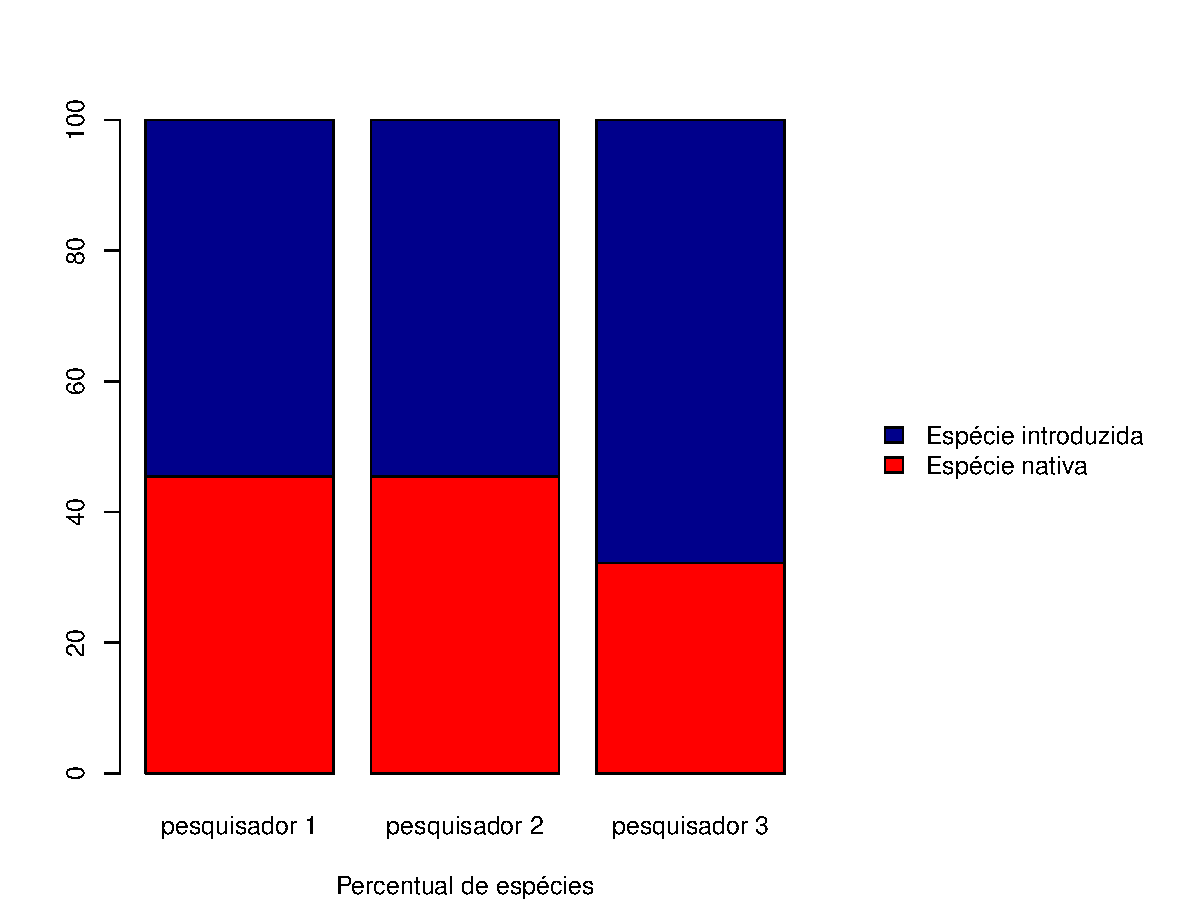
\includegraphics{livroR-1.0_files/figure-latex/bar-tab-1.pdf}
\caption{\label{fig:bar-tab}Gráfico de barras sobrepostas indicando o percentual relativo da observação de espécies nativas (cor vermelha) e introduzidas (cor azul), por pesquisador.}
\end{figure}

Como podem ver o nosso gráfico foi realizado. Mas adicionamos uma série de comandos novos. Vamos explica-lo passo a passo.

Primeiro contruímos a tabela com os dados em percentuais relativos ao pesquisador e o armazenamos em um objeto chamado tabela.

Posteriormente utilizamos uma função chamada \emph{par()} com o argumento mar no qual concatenamos 4 valores. Esta função juntamente com esse argumento permite que redimensionemos a janela gráfica. Os quatro valores concatenados referem-se as margens inferior, esquerda, superior e direita, respectivamente.

Nosso último passo é a nossa já conhecida função \emph{barplot()}, onde inserimos como primeiro valor o objeto que contem os dados que queremos graficar ``tabela'', seguido pelo argumento ``col'' que define as cores de acordo com as linhas da tabela, por sua vez definimos se a legenda será plotada com o argumento ``legend.text'' e por último indicamos a posição e o formato da legenda por meio do argumento ``args.lengend''. Neste último argumento precisamos inserir uma função list no qual indicamos a posição da legenda pelo argumento ``x'', o argumento ``bty'' o qual define que a legenda não tera uma caixa desenhada em seu entorno e o argumento ``inset'' que define a posição da legenda em relação ao eixo x.

Para plotar um gráfico via \emph{barplot()} a escrita pode ser feita de muitas maneiras, principalmente no que se refere a inserção da legenda. Experimente desenvolver um gráfico do mesmo estilo usando o conhecimento aprendido no capítulo anterior sobre gráficos.

\hypertarget{teste-t.}{%
\chapter{Teste-t.}\label{teste-t.}}

Ao iniciarmos nossos estudos geralmente estamos interessados em saber se alguma característica da população que coletamos e analisamos é similar a uma outra população. Podemos abordar essa ideia por diversos caminhos porém vamos iniciar nossas análises em R através do teste-t para uma amostra e a discussão sobre hipótese nula, caudalidade e nível de confiança. A partir de então seguiremos para o teste-t com duas amostras e o teste-t pareado.

\hypertarget{teste-t-para-uma-amostra}{%
\section{Teste-t para uma amostra}\label{teste-t-para-uma-amostra}}

Conduzimos esse teste quando objetivamos verificar se a média de uma dada variável é similar a um valor esperado. Ao falarmos de média percebemos que a variável com a qual estamos lidando é do tipo númerica ou inteiro (a diferença entre ambas consiste na presença de casas decimais), ou seja, quantitativo. Ao compararmos a média de nossa variável a um valor previamente estipulado 2 hipóteses são construídas, a hipótese nula (H0) e a hipótese alternativa (HA). H0 diz que a média de nossa variável é similar ao valor previamente estipulado, enquanto que HA diz que a média de nossa variável é diferente do valor previamente estipulado.

Matematicamente podemos obter o resultado do teste-t pela seguinte fórmula: \(t_s=(x-mi)/(s/sqrt(n))\). Onde, x: média da amostra, mi: média teórica esperada, s: desvio padrão da amostra, n: tamanho da amostra.

Vamos verificar como conduzir esse teste no R por meio de exemplos utilizando valores fictícios.

Imagine o seguinte exemplo: 100 camarões foram coletados em um estuário. Suas medidas em relação ao tamanho foram tomadas e deseja-se saber se o seu tamanho médio é similar ou não ao tamanho médio (25,80 mm) da mesma espécie observada em outro estuario.

A partir do exemplo acima podemos definir nossas hipóteses, onde.

H0: média observada igual à média esperada;

HA: média observada diferente da média esperada;

Vamos começar gerando os dados relativos ao tamanho observado dos camarões que coletamos

\begin{Shaded}
\begin{Highlighting}[]
\KeywordTok{set.seed}\NormalTok{(}\DecValTok{1234}\NormalTok{)}
\NormalTok{tamanho.camarao <-}\StringTok{ }\KeywordTok{rnorm}\NormalTok{(}\DataTypeTok{n =} \DecValTok{100}\NormalTok{) }\OperatorTok{+}\StringTok{ }\KeywordTok{runif}\NormalTok{(}\DataTypeTok{n =} \DecValTok{100}\NormalTok{, }\DataTypeTok{min =} \DecValTok{17}\NormalTok{, }\DataTypeTok{max =} \DecValTok{33}\NormalTok{)}
\end{Highlighting}
\end{Shaded}

A função \emph{set.seed()} define os números aleatórios que serão gerados. Dessa forma, quando aplicado essa função associada a um número comum, no caso ``1234'', os números gerados aqui serão os mesmos em qualquer lugar.

A nossa segunda linha de comando utiliza a função \emph{rnorm()} o qual gera números aleatórios considerando uma distribuição normal e soma esses valores gerados a uma distribuição uniforme gerada pela função \emph{runif()}. A estas funções adicionamos argumentos que definem a quantidade de números gerados (argumento ``n''), o valor mínimo que pode ser gerado (argumento ``min'') e o valor máximo que pode ser gerado (argumento ``max''). E guardamos o resultado obtido em um objeto chamado tamanho.camarao. Repare que o nome do objeto não apresenta espaços ou acentos, que pode gerar problemas e/ou dificuldades na condução das análises.

Vamos verificar o resultado. Basta digitarmos o nome do objeto.

\begin{Shaded}
\begin{Highlighting}[]
\NormalTok{tamanho.camarao}
\end{Highlighting}
\end{Shaded}

\begin{verbatim}
##   [1] 26.36501 25.73118 23.16434 26.93999 25.85006 29.22289 21.34791 22.92014
##   [9] 19.70599 31.88009 25.58378 20.48762 19.18464 29.19344 27.02799 31.80449
##  [17] 26.70808 27.30077 23.83039 33.02083 23.89138 17.01159 20.68980 22.81711
##  [25] 18.44307 23.54454 30.40893 21.37080 25.12759 23.97507 30.85514 25.59575
##  [33] 17.99771 29.42112 24.44470 19.22824 26.81323 20.57450 24.53800 32.36946
##  [41] 25.23524 19.84181 19.61879 27.74526 31.68906 23.66401 28.26906 24.93702
##  [49] 31.93121 29.25393 23.70445 25.96390 20.11329 20.45772 17.87934 26.57236
##  [57] 22.84551 16.27916 28.03817 24.16301 31.17074 20.02190 26.56155 20.62508
##  [65] 18.92214 20.38837 27.83197 18.62320 19.12094 29.29845 22.72270 28.68786
##  [73] 22.64878 30.43969 19.48136 24.94834 28.74896 24.99252 21.52521 22.19714
##  [81] 22.72903 23.69804 30.32393 29.37573 29.65554 22.18997 24.85922 21.19787
##  [89] 27.94906 28.93757 27.42930 23.87127 33.93523 21.89126 26.24338 29.48277
##  [97] 26.96407 19.72505 28.14750 24.06552
\end{verbatim}

Vamos observar as métricas e gráficos, conforme já fizemos nos capítulos anteriores, mas relativos ao objeto criado.

\begin{Shaded}
\begin{Highlighting}[]
\KeywordTok{mean}\NormalTok{(tamanho.camarao)}
\end{Highlighting}
\end{Shaded}

\begin{verbatim}
## [1] 24.86218
\end{verbatim}

\begin{Shaded}
\begin{Highlighting}[]
\KeywordTok{min}\NormalTok{(tamanho.camarao)}
\end{Highlighting}
\end{Shaded}

\begin{verbatim}
## [1] 16.27916
\end{verbatim}

\begin{Shaded}
\begin{Highlighting}[]
\KeywordTok{max}\NormalTok{(tamanho.camarao)}
\end{Highlighting}
\end{Shaded}

\begin{verbatim}
## [1] 33.93523
\end{verbatim}

\begin{Shaded}
\begin{Highlighting}[]
\KeywordTok{length}\NormalTok{(tamanho.camarao)}
\end{Highlighting}
\end{Shaded}

\begin{verbatim}
## [1] 100
\end{verbatim}

\begin{Shaded}
\begin{Highlighting}[]
\KeywordTok{hist}\NormalTok{(tamanho.camarao)}
\end{Highlighting}
\end{Shaded}

\begin{figure}
\centering
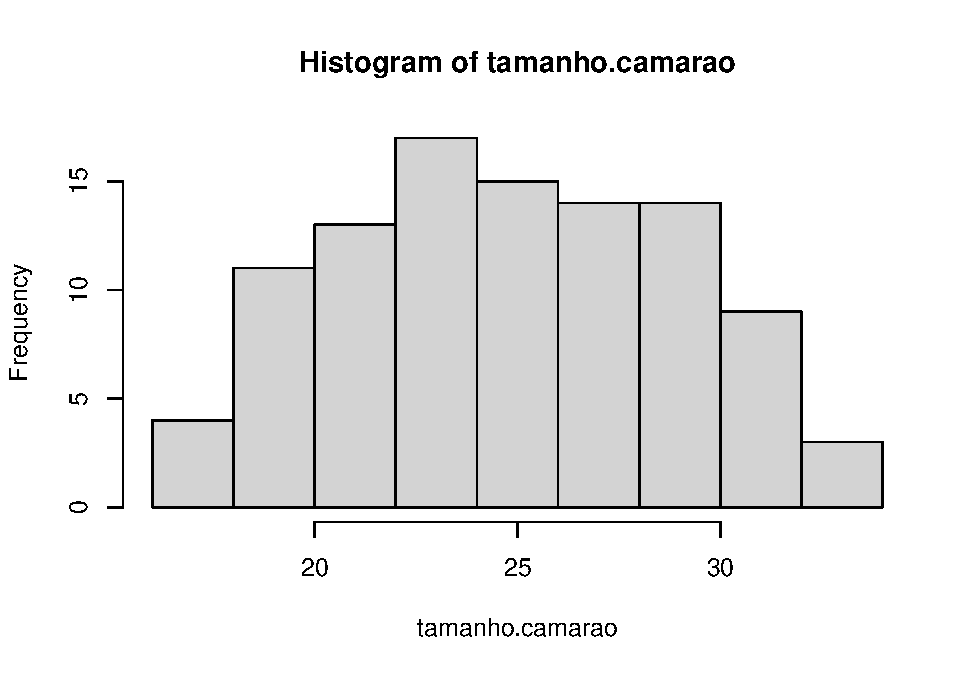
\includegraphics{livroR-1.0_files/figure-latex/hist-tam-cam-1.pdf}
\caption{\label{fig:hist-tam-cam}Histograma dos valores do objeto relativo ao tamanho dos camarões}
\end{figure}

Como podemos ver os valores mínimo e máximo são similares ao que definimos e o número de elementos é o mesmo. Graficamente podemos ver que a distribuição é normal, pois como vimos utilizamos uma função que cria uma distribuição normal com limites definidos pela função \emph{runif()}. Além disso vemos que há uma maior frequência dos valores em torno de 25 (Figura \ref{fig:hist-tam-cam}).

Vamos verificar, agora se esse valor que geramos (obtivemos de tamanho do camarão) são similares ao observado em outra localidade, por meio do teste-t para uma amostra.

\begin{Shaded}
\begin{Highlighting}[]
\NormalTok{esperado =}\StringTok{ }\FloatTok{25.80}
\KeywordTok{t.test}\NormalTok{(}\DataTypeTok{x =}\NormalTok{ tamanho.camarao, }\DataTypeTok{mu =}\NormalTok{ esperado)}
\end{Highlighting}
\end{Shaded}

\begin{verbatim}
## 
##  One Sample t-test
## 
## data:  tamanho.camarao
## t = -2.2432, df = 99, p-value = 0.02711
## alternative hypothesis: true mean is not equal to 25.8
## 95 percent confidence interval:
##  24.03263 25.69173
## sample estimates:
## mean of x 
##  24.86218
\end{verbatim}

Dois comandos foram executados, no primeiro criamos um objeto, denominado ``esperado'', que guarda o valor referente ao tamanho de camarão observado em outro estuário (25,80 mm). O segundo comando que realizamos refere-se a função do teste-t no qual inserimos 2 argumentos. O primeiro argumento (x) refere-se ao nosso objeto que contem os dados referentes ao tamanho que coletamos e o segundo argumento (mu) refere-se ao objeto que contem a média do tamanho obtido em outro estuário.

Conforme podemos visualizar no resultado temos 9 linhas. A primeira linha nos diz qual teste está sendo conduzido, neste caso é (``One Sample t-test'' ou teste-t par auma amostra), a segunda linha nos retorna o conjunto de dados que utilizamos, a terceira linha nos retorna o valor do teste t (t = -2,2432) o grau de liberdade (df = 99) e o valor de probabilidade associado ao teste (p-value = 0,02711), a quarta linha nos retorna qual é nossa hipótese alternativa, caso a aceitemos (a qual nos diz que: a média dos nossos dados não é igual à 25,8), a quinta e sexta linhas nos fornece o intervalo de confiança de 95\% dos nossos dados (24,03263 e 25,69173) e da sétima a nona linha refere-se a informação relativa a média dos nossos dados (24,86218).

Em resumo, podemos inferir que a média dos nossos dados é diferente do valor esperado pois o p-value foi menor que 0,05. Além disso podemos dizer que a média do tamanho dos camarões que coletamos (24,86 mm) é estatisticamente menor do que a média presente no outro estuário (25,80 mm). De outra forma podemos dizer que se rejeitarmos H0 cometeremos um erro de 1,5\% (p-value em percentual), ou seja, 1,5\% de estarmos cometendo o erro tipo 1 (rejeitar a H0 quando ela é verdadeira), como 1,5\% é menor que 5\%, temos subsídio para afirmar que a média obtida (24,86 mm) é diferente da média esperada (25,80 mm) (98,5\% de certeza).

Ok, verificamos e entendemos como conduzir a análise. Mas há um conceito estatístico importante na análise do teste-t, a caudalidade. No exemplo anterior nós trabalhamos com as hipóteses de que a média de um conjunto de dados é igual (H0) ou diferente (HA) da média esperada. O que implica em dizer que a média que observamos pode ser maior ou menor do que o esperado. Contudo em algumas instâncias podemos querer verificar se a média do nosso conjunto de dados é maior ou igual ou menor ou igual a média esperada e não diferente. Desta diferença na construção da hipótese que emerge o conceito da caudalidade. No exemplo anterior foi testado a hipótese bicaudal que é tido como padrão (``default'') na função do R que executamos.

A diferença entre realizar o teste-t bicaudal ou unicaudal depende da pergunta feita previamente e dos dados coletados. Então antes de realizar este teste mantenha-se atento a hipótese que se deseja testar.

Agora imagine o seguinte exemplo: Em um costão rochoso foi observado ao longo do dia ``1'' 100 estrelas do mar em diferentes alturas, em relação a baixamar. Essas alturas foram quantificadas (valores serão construídos abaixo). Sabe-se que no dia anterior ``0'' a altura média das estrelas no mesmo costão foi de 0,90 m. Sabe-se também que o dia anterior (dia 0) foi mais frio e que dias mais frios implicam em maiores alturas. A partir dessas informações e quais são as hipóteses testadas e o resultado do teste-t.

H0: A média da altura das estrelas do mar no costão no dia ``1'' é menor ou igual ao dia ``0''

HA: A média da altura das estrelas do mar no costão no dia ``1'' é maior que a do dia ``0''

Matematicamente podemos escrever da seguinte forma:

H0: μ ≤ 0,90

HA: μ \textgreater{} 0,90

\begin{Shaded}
\begin{Highlighting}[]
\KeywordTok{set.seed}\NormalTok{(}\DecValTok{1234}\NormalTok{)}
\NormalTok{estrelas <-}\StringTok{ }\KeywordTok{rnorm}\NormalTok{(}\DataTypeTok{n =} \DecValTok{100}\NormalTok{, }\DataTypeTok{sd =} \FloatTok{0.02}\NormalTok{) }\OperatorTok{+}\StringTok{ }\KeywordTok{runif}\NormalTok{(}\DataTypeTok{n =} \DecValTok{100}\NormalTok{, }\DataTypeTok{min =} \FloatTok{0.4}\NormalTok{, }\DataTypeTok{max =} \FloatTok{1.3}\NormalTok{)}
\end{Highlighting}
\end{Shaded}

Observe que geramos os dados de maneira similar ao que fizemos no exemplo anterior (inserindo os valores das alturas das estrelas em um objeto chamado estrelas), a diferença é que inserimos um argumento na função \emph{rnorm()} que corresponde ao desvio padrão (de 0,02) dos dados normais que estamos gerando.

\begin{Shaded}
\begin{Highlighting}[]
\KeywordTok{mean}\NormalTok{(estrelas)}
\end{Highlighting}
\end{Shaded}

\begin{verbatim}
## [1] 0.8479302
\end{verbatim}

\begin{Shaded}
\begin{Highlighting}[]
\KeywordTok{min}\NormalTok{(estrelas)}
\end{Highlighting}
\end{Shaded}

\begin{verbatim}
## [1] 0.387487
\end{verbatim}

\begin{Shaded}
\begin{Highlighting}[]
\KeywordTok{max}\NormalTok{(estrelas)}
\end{Highlighting}
\end{Shaded}

\begin{verbatim}
## [1] 1.290766
\end{verbatim}

\begin{Shaded}
\begin{Highlighting}[]
\KeywordTok{length}\NormalTok{(estrelas)}
\end{Highlighting}
\end{Shaded}

\begin{verbatim}
## [1] 100
\end{verbatim}

\begin{Shaded}
\begin{Highlighting}[]
\KeywordTok{hist}\NormalTok{(estrelas)}
\end{Highlighting}
\end{Shaded}

\begin{figure}
\centering
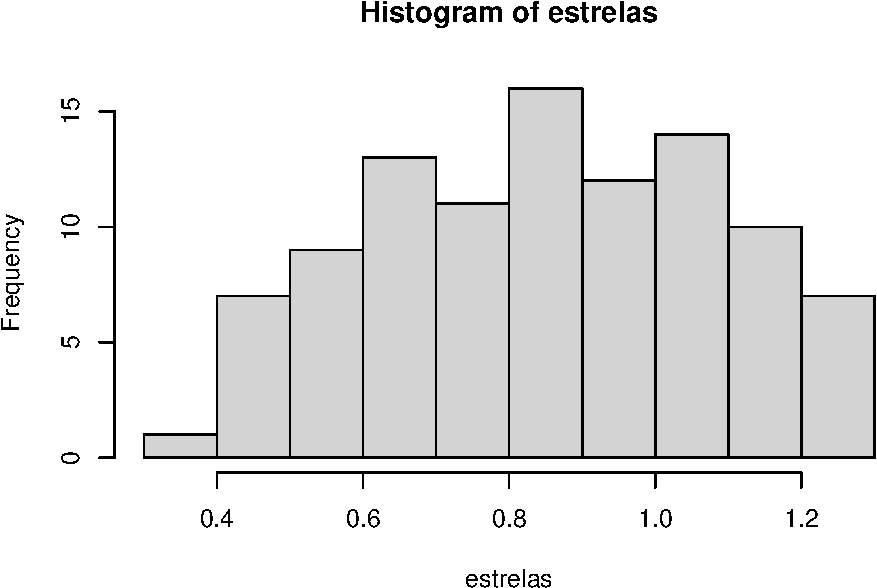
\includegraphics{livroR-1.0_files/figure-latex/estrelas-hist-1.pdf}
\caption{\label{fig:estrelas-hist}Histograma dos valores relativos a altura das estrelas do mar no costão rochoso}
\end{figure}

Conforme também fizemos anteriormente calculamos algumas métricas para entender os dados e um histograma básico (Figura \ref{fig:estrelas-hist}) para visualizar a forma dos dados que representam a altura que as estrelas se encontram no ambiente.

\begin{Shaded}
\begin{Highlighting}[]
\NormalTok{dia}\FloatTok{.0}\NormalTok{ =}\StringTok{ }\FloatTok{0.90}
\KeywordTok{t.test}\NormalTok{(}\DataTypeTok{x =}\NormalTok{ estrelas, }\DataTypeTok{mu =}\NormalTok{ dia}\FloatTok{.0}\NormalTok{, }\DataTypeTok{alternative =} \StringTok{"greater"}\NormalTok{)}
\end{Highlighting}
\end{Shaded}

\begin{verbatim}
## 
##  One Sample t-test
## 
## data:  estrelas
## t = -2.2073, df = 99, p-value = 0.9852
## alternative hypothesis: true mean is greater than 0.9
## 95 percent confidence interval:
##  0.8087617       Inf
## sample estimates:
## mean of x 
## 0.8479302
\end{verbatim}

Agora construímos um objeto chamado ``dia.0'' que nos retorna o valor médio encontrado para altura das estrelas do mar no costão no dia 0 e seguimos com o teste-t onde avaliamos se os dados que obtivemos do dia 1 são menores ou iguais ao dia 0, por meio do argumento ``alternative'' definido-o como ``greater''. Este argumento novo que incluímos pode ser definido de 3 formas: ``two-sided'' que é o padrão (``default''), ``greater'' ou ``less''. O argumento ``alternative'' seguirá o sinal da hipótese alternativa que foi construída para o teste.

Com isso podemos avaliar o resultado que é similar ao que vimos anteriormente com poucas mudanças. A primeira linha (One Sample t-test) informa sobre o teste realizado. A segunda linha indica o nome do conjunto de dados que inserimos. A terceira linha nos dá o valor do teste-t (t = -2,2073), do grau de liberdade (df = 99) e da probabilidade associada ao teste (p-value = 0.9852). A quarta linha indica a hipótese alternativa, caso seja aceita (o que não é o caso), que é verdade que a média dos nossos dados são maiores que 0,90 m. A quinta e sexta linha indicam o intervalo de confiança de 95\% dos nossos dados (0,8087617 e inf). A sétima, oitava e nona linha referem-se a média dos dados.

Como podemos notar pelo p-value do nosso resultado este demonstra que não temos informação o suficiente para rejeitar nossa hipótese nula (H0). Portanto a média dos nossos dados é menor ou igual a 0,90.

Outro conceito importante de qualquer teste inferencial (ex. teste-t) é o nível de confiança. Até o presente momento consideramos o nível de confiança de 95\%. Se quisermos altera-lo no teste-t devemos adicionar o argumento ``conf.level'' em proporção (0-1). A sua alteração implica na alteração da zona de rejeição da hipótese nula. Se aumentarmos o seu valor fica mais dificil rejeitarmos a hipótese nula e se diminuirmos o seu valor fica mais fácil rejeitar a hipótese nula. Vejamos outro exemplo.

Imagine o seguinte exemplo: Um pesquisador avaliou o tamanho de cracas incrustados no casco de uma embarcação. Objetivando saber se o tamanho médio de cracas difere do teórico esperado (20 mm) um teste-t bicaudal foi aplicado a um nível de confiança de 95\% e 99\%.

Vamos descrever as hipóteses e realizar a análise para ambos os níveis de confiança.

Neste caso temos as seguintes hipóteses:

H0: O tamanho médio observado é similar ao teórico

HA: O tamanho médio observado difere do teórico

Conforme já realizado anteriormente vamos gerar os dados e explora-los com algumas métricas estatśticas e gráficas de maneira similar ao que fizemos no exemplo anterior.

\begin{Shaded}
\begin{Highlighting}[]
\KeywordTok{set.seed}\NormalTok{(}\DecValTok{1234}\NormalTok{)}
\NormalTok{cracas <-}\StringTok{ }\KeywordTok{rnorm}\NormalTok{(}\DataTypeTok{n =} \DecValTok{100}\NormalTok{, }\DataTypeTok{sd =} \FloatTok{1.9}\NormalTok{) }\OperatorTok{+}\StringTok{ }\KeywordTok{runif}\NormalTok{(}\DataTypeTok{n =} \DecValTok{100}\NormalTok{, }\DataTypeTok{min =} \DecValTok{5}\NormalTok{, }\DataTypeTok{max =} \DecValTok{25}\NormalTok{)}

\KeywordTok{mean}\NormalTok{(cracas)}
\end{Highlighting}
\end{Shaded}

\begin{verbatim}
## [1] 14.72583
\end{verbatim}

\begin{Shaded}
\begin{Highlighting}[]
\KeywordTok{min}\NormalTok{(cracas)}
\end{Highlighting}
\end{Shaded}

\begin{verbatim}
## [1] 3.596275
\end{verbatim}

\begin{Shaded}
\begin{Highlighting}[]
\KeywordTok{max}\NormalTok{(cracas)}
\end{Highlighting}
\end{Shaded}

\begin{verbatim}
## [1] 27.27792
\end{verbatim}

\begin{Shaded}
\begin{Highlighting}[]
\KeywordTok{length}\NormalTok{(cracas)}
\end{Highlighting}
\end{Shaded}

\begin{verbatim}
## [1] 100
\end{verbatim}

\begin{Shaded}
\begin{Highlighting}[]
\KeywordTok{hist}\NormalTok{(cracas)}
\end{Highlighting}
\end{Shaded}

\begin{figure}
\centering
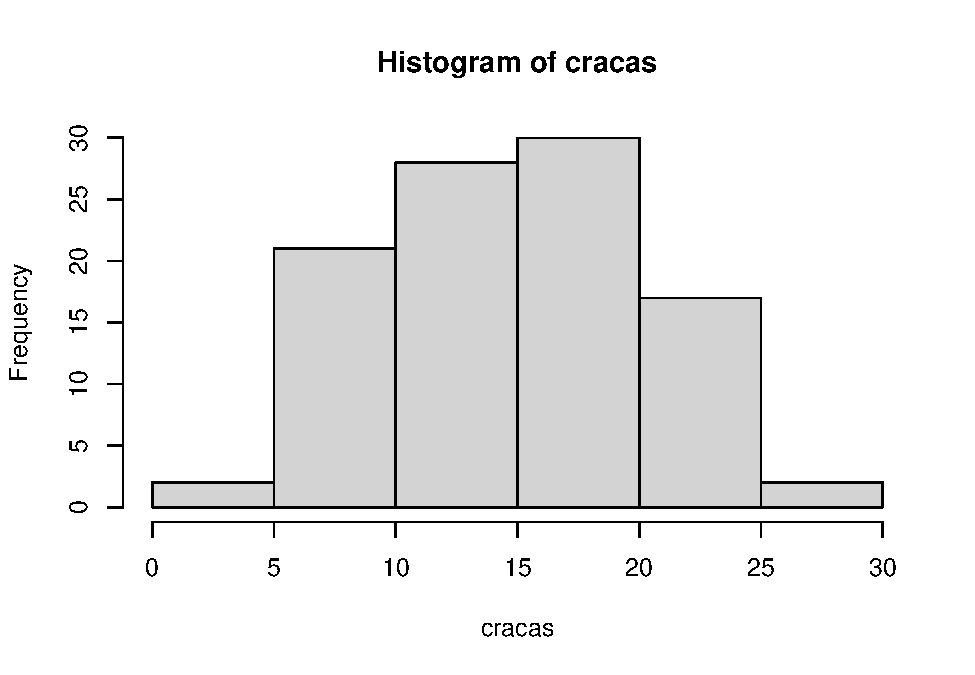
\includegraphics{livroR-1.0_files/figure-latex/craca-hist-1.pdf}
\caption{\label{fig:craca-hist}Histograma dos valores relativos ao tambanho das cracas incrustantes}
\end{figure}

Agora que visualizamos as métricas e graficamos os dados (Figura \ref{fig:craca-hist}), sigamos com a condução da análise.

\begin{Shaded}
\begin{Highlighting}[]
\NormalTok{teorico <-}\StringTok{ }\FloatTok{13.5}
\KeywordTok{t.test}\NormalTok{(}\DataTypeTok{x =}\NormalTok{ cracas, }\DataTypeTok{mu =}\NormalTok{ teorico, }\DataTypeTok{conf.level =} \FloatTok{0.95}\NormalTok{)}
\end{Highlighting}
\end{Shaded}

\begin{verbatim}
## 
##  One Sample t-test
## 
## data:  cracas
## t = 2.3113, df = 99, p-value = 0.02289
## alternative hypothesis: true mean is not equal to 13.5
## 95 percent confidence interval:
##  13.67349 15.77817
## sample estimates:
## mean of x 
##  14.72583
\end{verbatim}

\begin{Shaded}
\begin{Highlighting}[]
\KeywordTok{t.test}\NormalTok{(}\DataTypeTok{x =}\NormalTok{ cracas, }\DataTypeTok{mu =}\NormalTok{ teorico, }\DataTypeTok{conf.level =} \FloatTok{0.99}\NormalTok{)}
\end{Highlighting}
\end{Shaded}

\begin{verbatim}
## 
##  One Sample t-test
## 
## data:  cracas
## t = 2.3113, df = 99, p-value = 0.02289
## alternative hypothesis: true mean is not equal to 13.5
## 99 percent confidence interval:
##  13.33290 16.11876
## sample estimates:
## mean of x 
##  14.72583
\end{verbatim}

Como podem ver ambos os resultados (com diferentes níveis de confiança) retornam o mesmo valor do teste-t e do ``p-value''. E neste ponto precisamos ir com calma para evitar erro de interpretação do resultado e entender estatisticamente o que está acontencendo.

Quando representamos o nível de confiança (representado pelo argumento ``conf.level'') por um valor probabilístico de 0,95 ou 0,99 estamos dizendo que o nível de significância é 0,05 e 0,01, respectivamente. Quando olhamos para o resultado do p-value, temos que levar em consideração o nível de significância (que consiste em: 1 - nível de confiança).

Vejamos o nosso resultado.

No primeiro caso (``conf.level = 0.95'') temos p-value = 0.02289, como este valor é menor que 0,05 (nosso nível de significância), isso quer dizer que a média teórica está fora do intervalo de confiança dos dados, portanto rejeitamos a hipótese nula.

No segundo caso (``conf.level = 0.99'') temos o mesmo ``p-value'', contudo este valor é maior que nosso nível de significância (0,01), isso quer dizer que nossa média teórica está dentro do intervalo de confiança, portanto aceitamos a hipótese nula de que a média observada é similar a média teórica.

O nível de significância a aplicar nos seus dados depende das informações que possui sobre o organismo e o ambiente que está estudando. Apesar da regra-de-bolso dizer 0,05 e por padrão o R definir esse nível de significância é necessário discutir o que ele representa para seus dados e qual a implicação para sua hipótese e as medidas que serão tomadas. Uma dica importante é: reporte sempre o intervalo de confiança, indique o nível de significância (consiste em: 1 menos o nível de confiança) que foi aplicado e no seu texto deixe claro a escolha do nível de significância, principalmente se for diferente do que é definido como padrão.

\textbf{BÔNUS:}

Embora não seja comum, podemos plotar um gráfico que represente o nosso resultado estatístico como uma curva de densidade no qual é representado o valor do teste-t, o grau de liberdade e o valor de probabilidade associado. Para isso vamos usar um pacote o qual precisa ser instalado chamado ``webr'' e precisamos carrega-lo usando a função library(). Após isso é só inserir a função que desenvolve o teste-t dentro da função plot(). Veja o resultado para ambos os níveis de confiança estabelecidos previamente. OBS: Uma vez instalado o pacote não precisa instala-lo novamente.

\begin{Shaded}
\begin{Highlighting}[]
\CommentTok{## install.packages("webr")}
\KeywordTok{library}\NormalTok{(webr)}
\end{Highlighting}
\end{Shaded}

\begin{Shaded}
\begin{Highlighting}[]
\KeywordTok{plot}\NormalTok{(}\KeywordTok{t.test}\NormalTok{(}\DataTypeTok{x =}\NormalTok{ cracas, }\DataTypeTok{mu =}\NormalTok{ teorico, }\DataTypeTok{conf.level =} \FloatTok{0.95}\NormalTok{))}
\end{Highlighting}
\end{Shaded}

\begin{figure}
\centering
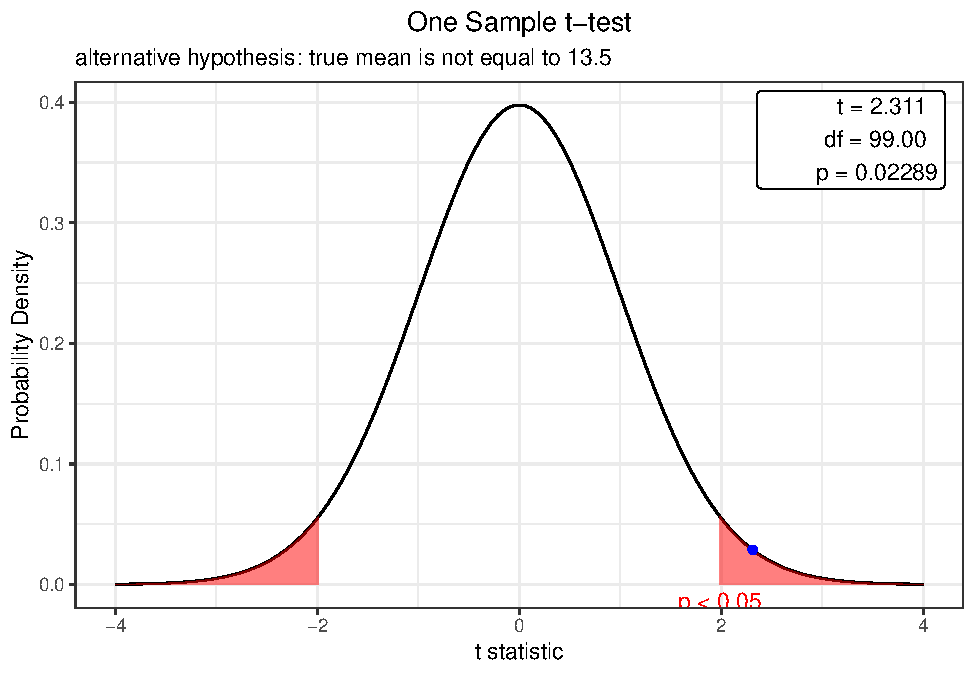
\includegraphics{livroR-1.0_files/figure-latex/cracas-dens-95-1.pdf}
\caption{\label{fig:cracas-dens-95}Curva de densidade representando o valor do teste-t bicaudal para o tamanho das cracas em relação a média teórica a um intervalo de confiança de 95\%. O ponto azul indica o valor do teste.}
\end{figure}

\begin{Shaded}
\begin{Highlighting}[]
\KeywordTok{plot}\NormalTok{(}\KeywordTok{t.test}\NormalTok{(}\DataTypeTok{x =}\NormalTok{ cracas, }\DataTypeTok{mu =}\NormalTok{ teorico, }\DataTypeTok{conf.level =} \FloatTok{0.99}\NormalTok{))}
\end{Highlighting}
\end{Shaded}

\begin{figure}
\centering
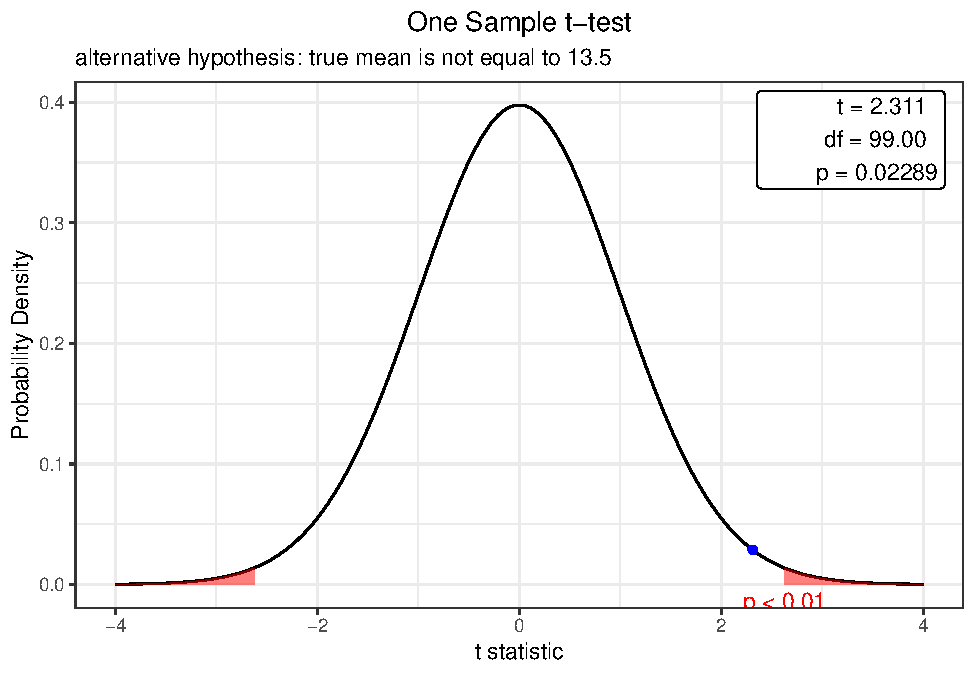
\includegraphics{livroR-1.0_files/figure-latex/cracas-dens-99-1.pdf}
\caption{\label{fig:cracas-dens-99}Curva de densidade representando o valor do teste-t bicaudal para o tamanho das cracas em relação a média teórica a um intervalo de confiança de 99\%. O ponto azul indica o valor do teste.}
\end{figure}

Verifique que esses plots nos fornecem as curvas do teste-t aos intervaloe de confiança de 95\% (Figura \ref{fig:cracas-dens-95}) e 99\% (Figura \ref{fig:cracas-dens-99}), demarca os limites inferior e superior de vermelho e marca como ponto azul na curva de densidade o valor do teste-t associado. Como esse valor está dentro da região demarcada no intervalo de confiança de 95\%, neste caso rejeitamos a hipótese nula e como no intervalo de confiança de 99\% o ponto azul está fora da região demarcada aceitamos a hipótese nula.

\hypertarget{teste-t-para-duas-amostras}{%
\section{Teste-t para duas amostras}\label{teste-t-para-duas-amostras}}

Conduzimos esse teste quando objetivamos comparar se a média de dois grupos (= amostras, populações etc) são similares. Portanto para sua realização é necessário uma variável mensurável e uma variável categórica com 2 grupos.

Ou seja, partindo desse objetivo as hipóteses nula e alternativa desse teste são as seguintes:

H0: A diferença na média da variável quantitativa dos grupos é igual a 0;

HA: A diferença na média da variável quantitativa dos grupos é diferente de 0;

Outra forma de apresentarmos a hipótese relativa a esste teste é:

H0: A média da variável quantitativa é igual entre grupos;

HA: A média da variável quantitativa é diferente entre grupos;

Outra forma de escrevermos a hipótese é em relação a caudalidade do teste e, se unicaudal, pode ser escrita da seguinte forma:

H0: A média da variável quantitativa é maior ou igual (ou menor ou igual) entre grupos;

HA: A média da variável quantitativa é menor (ou maior) entre grupos;

A partir desse teste alguns pressupostos estatísticos precisam ser avaliados e portanto algumas análises precisam ser realizadas antes da interpretação do resultado do teste-t. Pressupostos como normalidade (ambos os grupos devem provir de uma população com distribuição normal) e homocedasticidade (A variância entre os dois grupos devem ser iguais). Demonstraremos a frente como realizar alguns desses testes. Mas, primeiro vamos gerar os dados a serem trabalhados para esta etapa. Execute o código abaixo e você irá visualizar no ``environment'' do seu RStudio um objeto chamado ``gastropode'' que corresponde a um data frame com o conjunto de dados que iremos trabalhar.

\begin{Shaded}
\begin{Highlighting}[]
\NormalTok{grupos <-}\StringTok{ }\KeywordTok{c}\NormalTok{(}\KeywordTok{rep}\NormalTok{(}\DataTypeTok{x =} \StringTok{"Alimento A"}\NormalTok{, }\DecValTok{50}\NormalTok{), }\KeywordTok{rep}\NormalTok{(}\DataTypeTok{x =} \StringTok{"Alimento B"}\NormalTok{, }\DecValTok{50}\NormalTok{))}
\KeywordTok{set.seed}\NormalTok{(}\DecValTok{123}\NormalTok{)}
\NormalTok{alimento.A <-}\StringTok{ }\KeywordTok{rnorm}\NormalTok{(}\DataTypeTok{n =} \DecValTok{50}\NormalTok{, }\DataTypeTok{mean =} \FloatTok{0.7}\NormalTok{, }\DataTypeTok{sd =} \FloatTok{0.2}\NormalTok{)}
\KeywordTok{set.seed}\NormalTok{(}\DecValTok{4321}\NormalTok{)}
\NormalTok{alimento.B <-}\StringTok{ }\KeywordTok{rnorm}\NormalTok{(}\DataTypeTok{n =} \DecValTok{50}\NormalTok{, }\DataTypeTok{mean =} \FloatTok{0.2}\NormalTok{, }\DataTypeTok{sd =} \FloatTok{0.2}\NormalTok{)}
\NormalTok{Alimento <-}\StringTok{ }\KeywordTok{c}\NormalTok{(alimento.A, alimento.B)}
\NormalTok{gastropode <-}\StringTok{ }\KeywordTok{as.data.frame}\NormalTok{(}\KeywordTok{cbind}\NormalTok{(grupos, }\KeywordTok{round}\NormalTok{(Alimento, }\DecValTok{3}\NormalTok{)))}
\KeywordTok{colnames}\NormalTok{(gastropode) <-}\StringTok{ }\KeywordTok{c}\NormalTok{(}\StringTok{"Alimento"}\NormalTok{, }\StringTok{"Peso"}\NormalTok{)}
\KeywordTok{rm}\NormalTok{(}\DataTypeTok{list =} \StringTok{"grupos"}\NormalTok{, }\StringTok{"alimento.A"}\NormalTok{, }\StringTok{"alimento.B"}\NormalTok{, }\StringTok{"Alimento"}\NormalTok{)}
\end{Highlighting}
\end{Shaded}

\textcolor{red}{Neste momento não entraremos em detalhes sobre os comandos aplicados para construção desses dados. Caso seja do seu interesse consulte o apêndice, no final do livro.}

Vamos, agora, verificar os dados por meio da função \emph{head()} e a estrutura dos dados por meio da função \emph{str()} e alterar a estrutura dos dados se necessário.

\begin{Shaded}
\begin{Highlighting}[]
\KeywordTok{head}\NormalTok{(gastropode)}
\end{Highlighting}
\end{Shaded}

\begin{verbatim}
##     Alimento  Peso
## 1 Alimento A 0.588
## 2 Alimento A 0.654
## 3 Alimento A 1.012
## 4 Alimento A 0.714
## 5 Alimento A 0.726
## 6 Alimento A 1.043
\end{verbatim}

\begin{Shaded}
\begin{Highlighting}[]
\KeywordTok{str}\NormalTok{(gastropode)}
\end{Highlighting}
\end{Shaded}

\begin{verbatim}
## 'data.frame':    100 obs. of  2 variables:
##  $ Alimento: chr  "Alimento A" "Alimento A" "Alimento A" "Alimento A" ...
##  $ Peso    : chr  "0.588" "0.654" "1.012" "0.714" ...
\end{verbatim}

\begin{Shaded}
\begin{Highlighting}[]
\NormalTok{gastropode}\OperatorTok{$}\NormalTok{Alimento <-}\StringTok{ }\KeywordTok{as.factor}\NormalTok{(gastropode}\OperatorTok{$}\NormalTok{Alimento)}
\NormalTok{gastropode}\OperatorTok{$}\NormalTok{Peso <-}\StringTok{ }\KeywordTok{as.numeric}\NormalTok{(gastropode}\OperatorTok{$}\NormalTok{Peso)}
\KeywordTok{str}\NormalTok{(gastropode)}
\end{Highlighting}
\end{Shaded}

\begin{verbatim}
## 'data.frame':    100 obs. of  2 variables:
##  $ Alimento: Factor w/ 2 levels "Alimento A","Alimento B": 1 1 1 1 1 1 1 1 1 1 ...
##  $ Peso    : num  0.588 0.654 1.012 0.714 0.726 ...
\end{verbatim}

Agora que importamos e organizamos nossa planilha vamos analisar nosso exemplo.

100 indivíduos de uma espécie de gastropode foi coletada e mantida em cultivo para avaliação da dieta. 50 indivíduos foram mantidos com uma dieta rica no Alimento A e 50 indivíduos com uma dieta rica no Alimento B. Todos os indivíduos foram pesados antes e depois do experimento. A planilha a seguir informa a alteração de peso dos organismos, em gramas, após a dieta oferecida.

Antes de conduzirmos o teste-t vamos praticar fazendo a avaliação gráfica e númerica dos dados.

\begin{Shaded}
\begin{Highlighting}[]
\KeywordTok{hist}\NormalTok{(gastropode}\OperatorTok{$}\NormalTok{Peso [gastropode}\OperatorTok{$}\NormalTok{Alimento }\OperatorTok{==}\StringTok{ "Alimento A"}\NormalTok{], }
     \DataTypeTok{xlab =} \StringTok{"Alteração do peso"}\NormalTok{, }
     \DataTypeTok{ylab =} \StringTok{"Frequência", }
\StringTok{     main = "}\NormalTok{Alimento A}\StringTok{", }
\StringTok{     ylim = c(0, 20),}
\StringTok{     xlim = c(-0.5, 1.5))}
\end{Highlighting}
\end{Shaded}

\begin{figure}
\centering
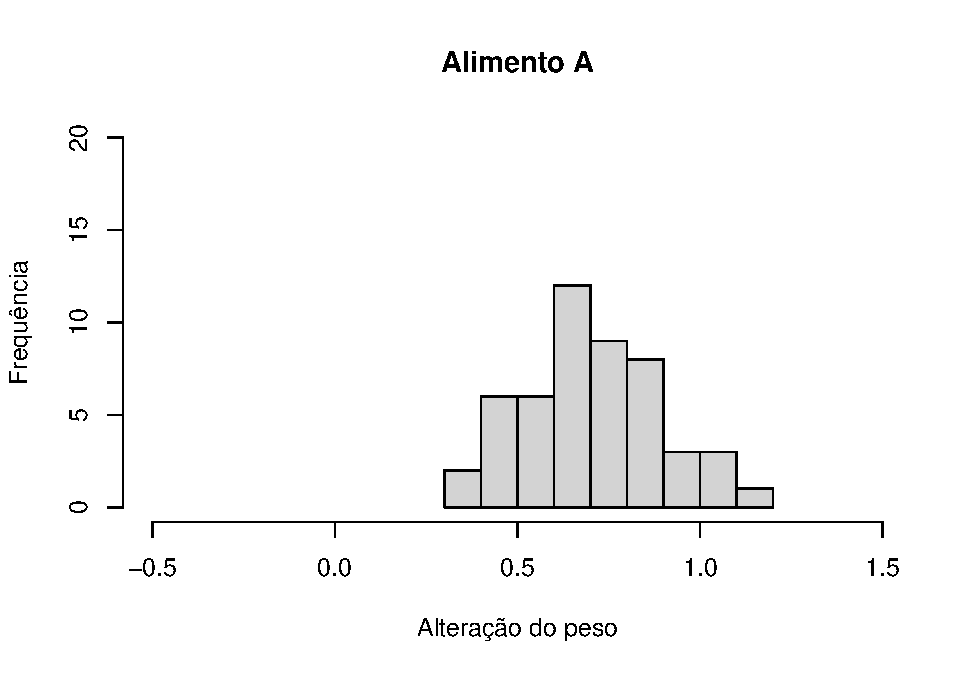
\includegraphics{livroR-1.0_files/figure-latex/hist-ali-A-1.pdf}
\caption{\label{fig:hist-ali-A}Histograma com valores da mudança do peso dos gastrópodes após a dieta com o Alimento A}
\end{figure}

\begin{Shaded}
\begin{Highlighting}[]
\KeywordTok{hist}\NormalTok{(gastropode}\OperatorTok{$}\NormalTok{Peso [gastropode}\OperatorTok{$}\NormalTok{Alimento }\OperatorTok{==}\StringTok{ "Alimento B"}\NormalTok{], }
     \DataTypeTok{xlab =} \StringTok{"Alteração do peso"}\NormalTok{, }
     \DataTypeTok{ylab =} \StringTok{"Frequência", }
\StringTok{     main = "}\NormalTok{Alimento B}\StringTok{",}
\StringTok{     ylim = c(0, 20),}
\StringTok{     xlim = c(-0.5, 1.5))}
\end{Highlighting}
\end{Shaded}

\begin{figure}
\centering
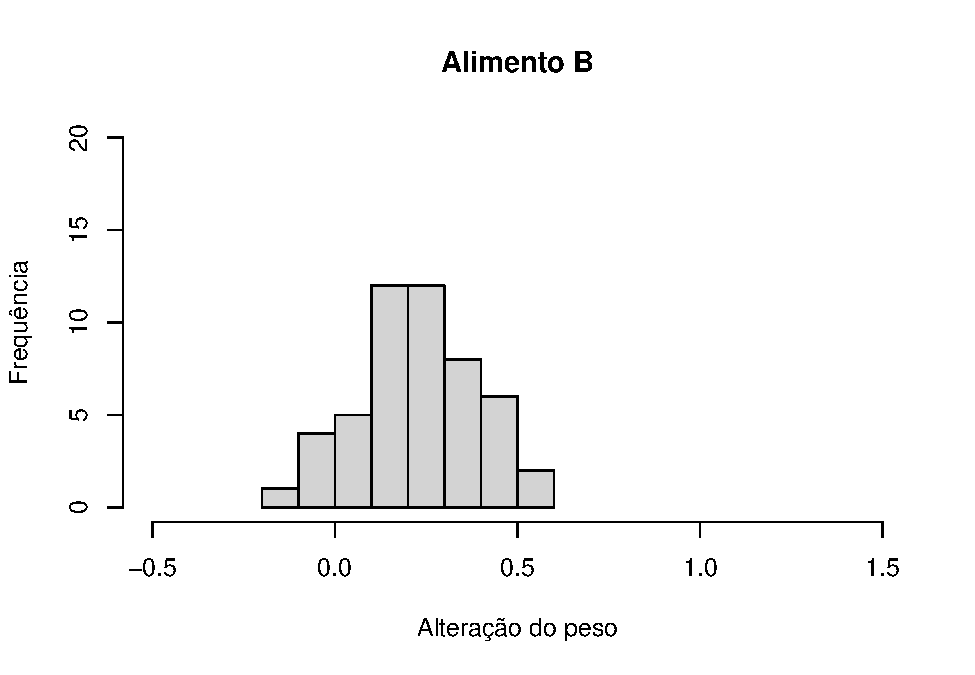
\includegraphics{livroR-1.0_files/figure-latex/hist-ali-B-1.pdf}
\caption{\label{fig:hist-ali-B}Histograma com valores da mudança do peso dos gastrópodes após a dieta com o Alimento B}
\end{figure}

\begin{Shaded}
\begin{Highlighting}[]
\KeywordTok{boxplot}\NormalTok{(Peso }\OperatorTok{~}\StringTok{ }\NormalTok{Alimento, }\DataTypeTok{data =}\NormalTok{ gastropode)}
\end{Highlighting}
\end{Shaded}

\begin{figure}
\centering
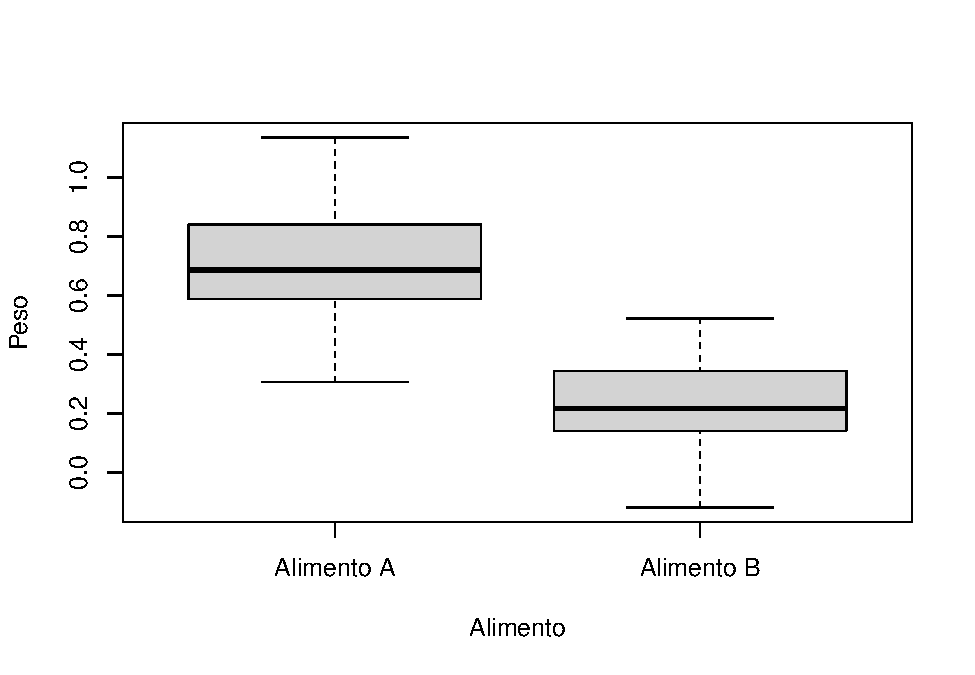
\includegraphics{livroR-1.0_files/figure-latex/box-ali-1.pdf}
\caption{\label{fig:box-ali}Boxplot com os valores da alteração do peso dos gastrópodes por tipo de alimento}
\end{figure}

Os comandos acima realizam: o histograma dos dados para Alimento A (Figura \ref{fig:hist-ali-A}), o histograma dos dados para Alimento B (Figura \ref{fig:hist-ali-B}) e o boxplot para ambos os dados (Figura \ref{fig:box-ali}), respectivamente.

Os 2 primeiros gráficos consistem em histogramas em relação aos dados de peso por Alimento. Na primeira linha indicamos a variável peso dentro da planilha gastropode por meio do operador matemático \$ (cifrão) e selecionamos os dados correspondentes ao Alimento utilizando colchetes {[}{]} dentro do qual selecionamos a variável Alimento dentro da planilha gastropode e por meio do sinal de igual duplicado (==) indicamos entre aspas ("``) o grupo (ou categoria) que desejamos. Os demais argumentos já são bem conhecidos e iguais para ambos os histogramas, diferindo apenas o título do gráfico que é definido pelo argumento''main".

O Boxplot resume os dados por Alimento e nos indica outras métricas (quartis), como vimos anteriormente no tópico sobre gráficos.

Mas se desejarmos observar os valores númericos que resumem os dados, podemos seguir o que aprendemos anteriormente.

\begin{Shaded}
\begin{Highlighting}[]
\KeywordTok{summary}\NormalTok{(gastropode)}
\end{Highlighting}
\end{Shaded}

\begin{verbatim}
##        Alimento       Peso        
##  Alimento A:50   Min.   :-0.1180  
##  Alimento B:50   1st Qu.: 0.2172  
##                  Median : 0.4475  
##                  Mean   : 0.4652  
##                  3rd Qu.: 0.6843  
##                  Max.   : 1.1340
\end{verbatim}

\begin{Shaded}
\begin{Highlighting}[]
\KeywordTok{mean}\NormalTok{(gastropode}\OperatorTok{$}\NormalTok{Peso)}
\end{Highlighting}
\end{Shaded}

\begin{verbatim}
## [1] 0.46519
\end{verbatim}

\begin{Shaded}
\begin{Highlighting}[]
\KeywordTok{mean}\NormalTok{(gastropode}\OperatorTok{$}\NormalTok{Peso [gastropode}\OperatorTok{$}\NormalTok{Alimento }\OperatorTok{==}\StringTok{ "Alimento A"}\NormalTok{])}
\end{Highlighting}
\end{Shaded}

\begin{verbatim}
## [1] 0.7069
\end{verbatim}

\begin{Shaded}
\begin{Highlighting}[]
\KeywordTok{mean}\NormalTok{(gastropode}\OperatorTok{$}\NormalTok{Peso [gastropode}\OperatorTok{$}\NormalTok{Alimento }\OperatorTok{==}\StringTok{ "Alimento B"}\NormalTok{])}
\end{Highlighting}
\end{Shaded}

\begin{verbatim}
## [1] 0.22348
\end{verbatim}

Utilizando o pacote Rmisc temos uma forma mais simples de escrita e eficiente para observar esses valores e algumas outras métricas (ex.: número amostral, média, desvio padrão, erro padrão e intervalo de confiança).

\begin{Shaded}
\begin{Highlighting}[]
\KeywordTok{library}\NormalTok{(Rmisc)}
\KeywordTok{summarySE}\NormalTok{(}\DataTypeTok{data =}\NormalTok{ gastropode, }\DataTypeTok{measurevar =} \StringTok{"Peso"}\NormalTok{, }\DataTypeTok{groupvars =} \StringTok{"Alimento"}\NormalTok{)}
\end{Highlighting}
\end{Shaded}

\begin{verbatim}
##     Alimento  N    Peso        sd         se         ci
## 1 Alimento A 50 0.70690 0.1852070 0.02619223 0.05263525
## 2 Alimento B 50 0.22348 0.1573551 0.02225337 0.04471982
\end{verbatim}

Ok, até aqui observamos como estão os nossos dados e podemos ver que a administração da Alimento A resultou em um maior ganho de peso pelos gastropodes do que a Alimento B. Mas será que o que observamos grafica e numericamente se reflete estatisticamente? Vamos a nossa avaliação dos pressupostos do teste-t para duas amostras e se cumpridos para a avaliação do teste-t.

Uma das formas mais convencionais de avaliar a normalidade é pelo teste de shapiro-wilks e a homocedasticidade pelo teste de Bartlett. Vamos avalia-las.

\begin{Shaded}
\begin{Highlighting}[]
\KeywordTok{shapiro.test}\NormalTok{(gastropode}\OperatorTok{$}\NormalTok{Peso [gastropode}\OperatorTok{$}\NormalTok{Alimento }\OperatorTok{==}\StringTok{ "Alimento A"}\NormalTok{])}
\end{Highlighting}
\end{Shaded}

\begin{verbatim}
## 
##  Shapiro-Wilk normality test
## 
## data:  gastropode$Peso[gastropode$Alimento == "Alimento A"]
## W = 0.98923, p-value = 0.9266
\end{verbatim}

\begin{Shaded}
\begin{Highlighting}[]
\KeywordTok{shapiro.test}\NormalTok{(gastropode}\OperatorTok{$}\NormalTok{Peso [gastropode}\OperatorTok{$}\NormalTok{Alimento }\OperatorTok{==}\StringTok{ "Alimento B"}\NormalTok{])}
\end{Highlighting}
\end{Shaded}

\begin{verbatim}
## 
##  Shapiro-Wilk normality test
## 
## data:  gastropode$Peso[gastropode$Alimento == "Alimento B"]
## W = 0.98059, p-value = 0.5769
\end{verbatim}

\begin{Shaded}
\begin{Highlighting}[]
\KeywordTok{bartlett.test}\NormalTok{(Peso }\OperatorTok{~}\StringTok{ }\NormalTok{Alimento, }\DataTypeTok{data =}\NormalTok{ gastropode)}
\end{Highlighting}
\end{Shaded}

\begin{verbatim}
## 
##  Bartlett test of homogeneity of variances
## 
## data:  Peso by Alimento
## Bartlett's K-squared = 1.2826, df = 1, p-value = 0.2574
\end{verbatim}

Como podemos observar, ambos os grupos apresentam dados normais e homocedásticos, para um nível de confiança de 95\%, já que o p-value foi superior a 0,05. Dessa forma vamos dar continuidade a nossa análise e verificar se as médias dos grupos são diferentes.

\begin{Shaded}
\begin{Highlighting}[]
\KeywordTok{t.test}\NormalTok{(Peso }\OperatorTok{~}\StringTok{ }\NormalTok{Alimento, }
       \DataTypeTok{data =}\NormalTok{ gastropode,}
       \DataTypeTok{var.equal =} \OtherTok{TRUE}\NormalTok{,}
       \DataTypeTok{conf.level =} \FloatTok{0.95}\NormalTok{)}
\end{Highlighting}
\end{Shaded}

\begin{verbatim}
## 
##  Two Sample t-test
## 
## data:  Peso by Alimento
## t = 14.065, df = 98, p-value < 2.2e-16
## alternative hypothesis: true difference in means is not equal to 0
## 95 percent confidence interval:
##  0.4152153 0.5516247
## sample estimates:
## mean in group Alimento A mean in group Alimento B 
##                  0.70690                  0.22348
\end{verbatim}

Repare que a forma da escrita se alterou um pouco. Mas como podem ver, nada complicado. Agora escrevemos a variável quantitativa (peso) em função da (\textasciitilde{}) variável categórica (Alimento). Guarde bem essa forma de escrita pois ela será utilizada para praticamente todos os testes a partir daqui e para inúmeras outras funções. Adcionamos o argumento ``data'' que indica a planilha de onde estamos utilizando as variáveis, o argumento ``var.equal'' o qual indica que a variância entre os grupos é igual e o argumento ``conf.level'' o qual define o nível de confiança com qual estamos trabalhando.

De acordo com nosso resultado podemos ver que o o valor do teste-t é 14,065, o grau de liberdade de 98 (o qual consiste no total de observações subtraído de um por grupo), o valor de probabilidade associado ao teste (\(2,2\times10^{-16}\)), o intervalo de confiança de 95\% (0,415 e 0,551) que refere-se a diferença da média entre os grupos (a diferença da média dos grupos é: 0,70690 - 0,22348 = 0,48342), ou seja, o intervalo de confiança é em função dessa diferença e as últimas linhas do resultado representam as médias de alteração do peso para cada Alimento (Alimento A = 0,70690 e Alimento B = 0,22348). De acordo com esse resultado refutamos a hipótese nula de que as médias são similares. Portanto podemos dizer que dependendo da Alimento (A ou B) utilizada na dieta podemos ter diferentes alterações no peso dos gastropodes.

Da mesma forma que avaliamos para o teste-t de uma amostra, podemos plotar o resultado como um gráfico da função de densidade do teste-t. Só devemos lembrar de carregar o pacote ``webr''.

\begin{Shaded}
\begin{Highlighting}[]
\KeywordTok{library}\NormalTok{(webr)}
\KeywordTok{plot}\NormalTok{(}\KeywordTok{t.test}\NormalTok{(Peso }\OperatorTok{~}\StringTok{ }\NormalTok{Alimento, }
            \DataTypeTok{data =}\NormalTok{ gastropode,}
            \DataTypeTok{var.equal =} \OtherTok{TRUE}\NormalTok{,}
            \DataTypeTok{conf.level =} \FloatTok{0.95}\NormalTok{))}
\end{Highlighting}
\end{Shaded}

\begin{figure}
\centering
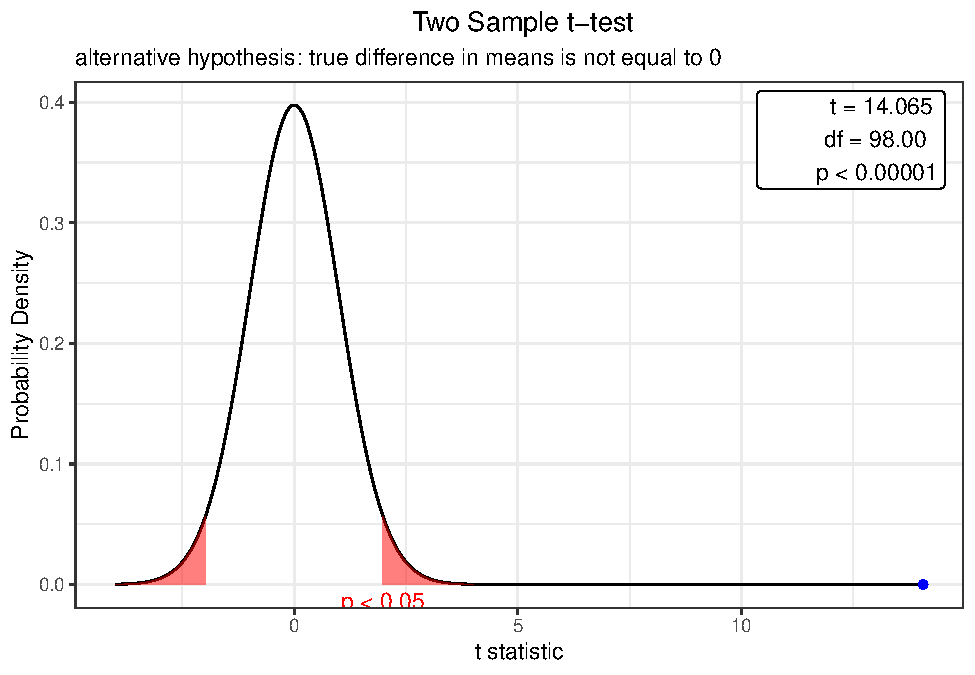
\includegraphics{livroR-1.0_files/figure-latex/testet-duas-dens-1.pdf}
\caption{\label{fig:testet-duas-dens}Curva de densidade representando o valor do teste-t bicaudal para a alteração do peso de gastrópodes em relação ao alimento a um intervalo de confiança de 95\%. O ponto azul indica o valor do teste.}
\end{figure}

Neste gráfico podemos ver que o resultado do teste-t (Figura \ref{fig:testet-duas-dens}), indicado pelo ponto azul, está muito além do nível da zona de rejeição, indicando que os dois grupos apresentam médias bem diferentes, ou seja, a diferença entre as duas médias é altamente significativa e diferente de 0.

Vamos exercitar nosso conhecimento em R e teste-t com um outro exemplo (Gere a planilha abaixo).

\begin{Shaded}
\begin{Highlighting}[]
\NormalTok{grupos <-}\StringTok{ }\KeywordTok{c}\NormalTok{(}\KeywordTok{rep}\NormalTok{(}\DataTypeTok{x =} \StringTok{"Ano 0"}\NormalTok{, }\DecValTok{36}\NormalTok{), }\KeywordTok{rep}\NormalTok{(}\DataTypeTok{x =} \StringTok{"Ano 20"}\NormalTok{, }\DecValTok{36}\NormalTok{))}
\KeywordTok{set.seed}\NormalTok{(}\DecValTok{245}\NormalTok{)}
\NormalTok{ano}\FloatTok{.0}\NormalTok{ <-}\StringTok{ }\KeywordTok{rnorm}\NormalTok{(}\DataTypeTok{n =} \DecValTok{36}\NormalTok{, }\DataTypeTok{mean =} \FloatTok{15.7}\NormalTok{, }\DataTypeTok{sd =} \FloatTok{0.2}\NormalTok{) }\OperatorTok{+}\StringTok{ }\KeywordTok{runif}\NormalTok{(}\DataTypeTok{n =} \DecValTok{36}\NormalTok{)}
\KeywordTok{set.seed}\NormalTok{(}\DecValTok{356}\NormalTok{)}
\NormalTok{ano}\FloatTok{.20}\NormalTok{ <-}\StringTok{ }\KeywordTok{rnorm}\NormalTok{(}\DataTypeTok{n =} \DecValTok{36}\NormalTok{, }\DataTypeTok{mean =} \FloatTok{16.2}\NormalTok{, }\DataTypeTok{sd =} \FloatTok{0.5}\NormalTok{) }\OperatorTok{+}\StringTok{ }\KeywordTok{runif}\NormalTok{(}\DataTypeTok{n =} \DecValTok{36}\NormalTok{)}
\NormalTok{ano <-}\StringTok{ }\KeywordTok{c}\NormalTok{(ano}\FloatTok{.0}\NormalTok{, ano}\FloatTok{.20}\NormalTok{)}
\NormalTok{lagoa <-}\StringTok{ }\KeywordTok{as.data.frame}\NormalTok{(}\KeywordTok{cbind}\NormalTok{(grupos, }\KeywordTok{round}\NormalTok{(ano, }\DecValTok{3}\NormalTok{)))}
\KeywordTok{colnames}\NormalTok{(lagoa) <-}\StringTok{ }\KeywordTok{c}\NormalTok{(}\StringTok{"Ano"}\NormalTok{, }\StringTok{"Temperatura"}\NormalTok{)}
\KeywordTok{rm}\NormalTok{(}\DataTypeTok{list =} \StringTok{"grupos"}\NormalTok{, }\StringTok{"ano.0"}\NormalTok{, }\StringTok{"ano.20"}\NormalTok{, }\StringTok{"ano"}\NormalTok{)}
\end{Highlighting}
\end{Shaded}

Imagine que durante um ano você mensurou a temperatura de uma lagoa três vezes por mês durante todos os meses ao longo de 1 ano. 20 anos depois você retornou a lagoa e mensurou novamente a temperatura três vezes por mês durante um ano. Considerando um nível de confiança de 99\% a temperatura é igual ou diferente entre os anos?

A primeira coisa que devemos fazer é escrever nossa hipótese. Vamos a ela.

H0: A média da temperatura é igual entre os anos;

HA: A média da temperatura é diferente entre os anos;

Com a hipótese construída vamos verificar a estrutura dos dados (modificar se necessário) e sumarizar nossos dados gráfica e matematicamente.

\begin{Shaded}
\begin{Highlighting}[]
\KeywordTok{head}\NormalTok{(lagoa)}
\end{Highlighting}
\end{Shaded}

\begin{verbatim}
##     Ano Temperatura
## 1 Ano 0      16.345
## 2 Ano 0      16.383
## 3 Ano 0      15.727
## 4 Ano 0      16.058
## 5 Ano 0      15.842
## 6 Ano 0      16.158
\end{verbatim}

\begin{Shaded}
\begin{Highlighting}[]
\KeywordTok{str}\NormalTok{(lagoa)}
\end{Highlighting}
\end{Shaded}

\begin{verbatim}
## 'data.frame':    72 obs. of  2 variables:
##  $ Ano        : chr  "Ano 0" "Ano 0" "Ano 0" "Ano 0" ...
##  $ Temperatura: chr  "16.345" "16.383" "15.727" "16.058" ...
\end{verbatim}

\begin{Shaded}
\begin{Highlighting}[]
\NormalTok{lagoa}\OperatorTok{$}\NormalTok{Ano <-}\StringTok{ }\KeywordTok{as.factor}\NormalTok{(lagoa}\OperatorTok{$}\NormalTok{Ano)}
\NormalTok{lagoa}\OperatorTok{$}\NormalTok{Temperatura <-}\StringTok{ }\KeywordTok{as.numeric}\NormalTok{(lagoa}\OperatorTok{$}\NormalTok{Temperatura)}
\KeywordTok{str}\NormalTok{(lagoa)}
\end{Highlighting}
\end{Shaded}

\begin{verbatim}
## 'data.frame':    72 obs. of  2 variables:
##  $ Ano        : Factor w/ 2 levels "Ano 0","Ano 20": 1 1 1 1 1 1 1 1 1 1 ...
##  $ Temperatura: num  16.3 16.4 15.7 16.1 15.8 ...
\end{verbatim}

\begin{Shaded}
\begin{Highlighting}[]
\KeywordTok{hist}\NormalTok{(lagoa}\OperatorTok{$}\NormalTok{Temperatura [lagoa}\OperatorTok{$}\NormalTok{Ano }\OperatorTok{==}\StringTok{ "Ano 0"}\NormalTok{], }
     \DataTypeTok{xlab =} \StringTok{"Temperatura (°C)"}\NormalTok{, }
     \DataTypeTok{ylab =} \StringTok{"Frequência", }
\StringTok{     main = "}\NormalTok{Ano }\DecValTok{0}\StringTok{", }
\StringTok{     ylim = c(0, 15),}
\StringTok{     xlim = c(15, 19))}
\end{Highlighting}
\end{Shaded}

\begin{figure}
\centering
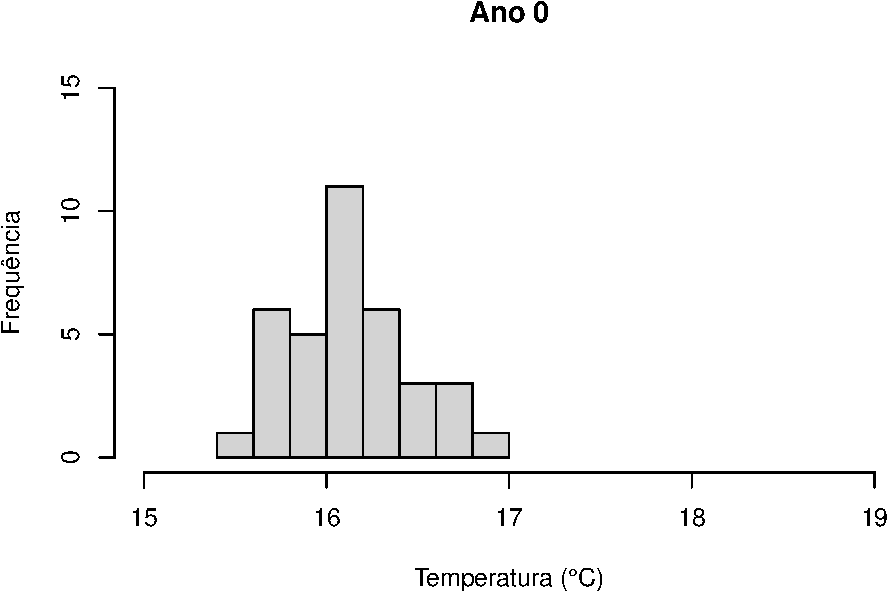
\includegraphics{livroR-1.0_files/figure-latex/hist-temp-0-1.pdf}
\caption{\label{fig:hist-temp-0}Histograma com valores de temperatura da lagoa no Ano 0.}
\end{figure}

\begin{Shaded}
\begin{Highlighting}[]
\KeywordTok{hist}\NormalTok{(lagoa}\OperatorTok{$}\NormalTok{Temperatura [lagoa}\OperatorTok{$}\NormalTok{Ano }\OperatorTok{==}\StringTok{ "Ano 20"}\NormalTok{], }
     \DataTypeTok{xlab =} \StringTok{"Temperatura (°C)"}\NormalTok{, }
     \DataTypeTok{ylab =} \StringTok{"Frequência", }
\StringTok{     main = "}\NormalTok{Ano }\DecValTok{20}\StringTok{", }
\StringTok{     ylim = c(0, 15),}
\StringTok{     xlim = c(15, 19))}
\end{Highlighting}
\end{Shaded}

\begin{figure}
\centering
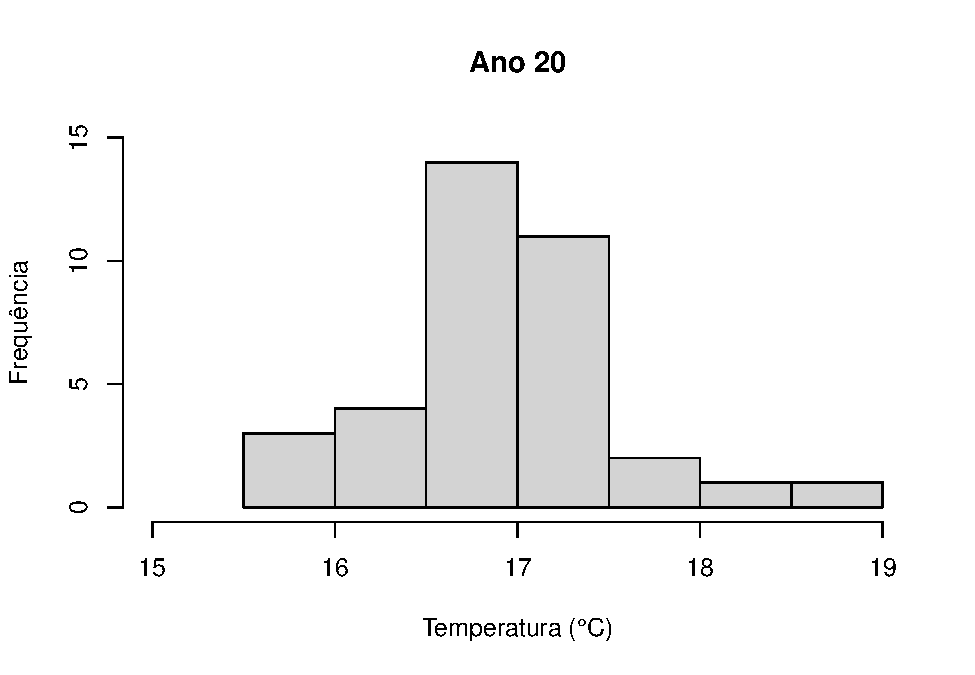
\includegraphics{livroR-1.0_files/figure-latex/hist-temp-20-1.pdf}
\caption{\label{fig:hist-temp-20}Histograma com valores de temperatura da lagoa no Ano 20.}
\end{figure}

\begin{Shaded}
\begin{Highlighting}[]
\KeywordTok{boxplot}\NormalTok{(Temperatura }\OperatorTok{~}\StringTok{ }\NormalTok{Ano, }\DataTypeTok{data =}\NormalTok{ lagoa)}
\end{Highlighting}
\end{Shaded}

\begin{figure}
\centering
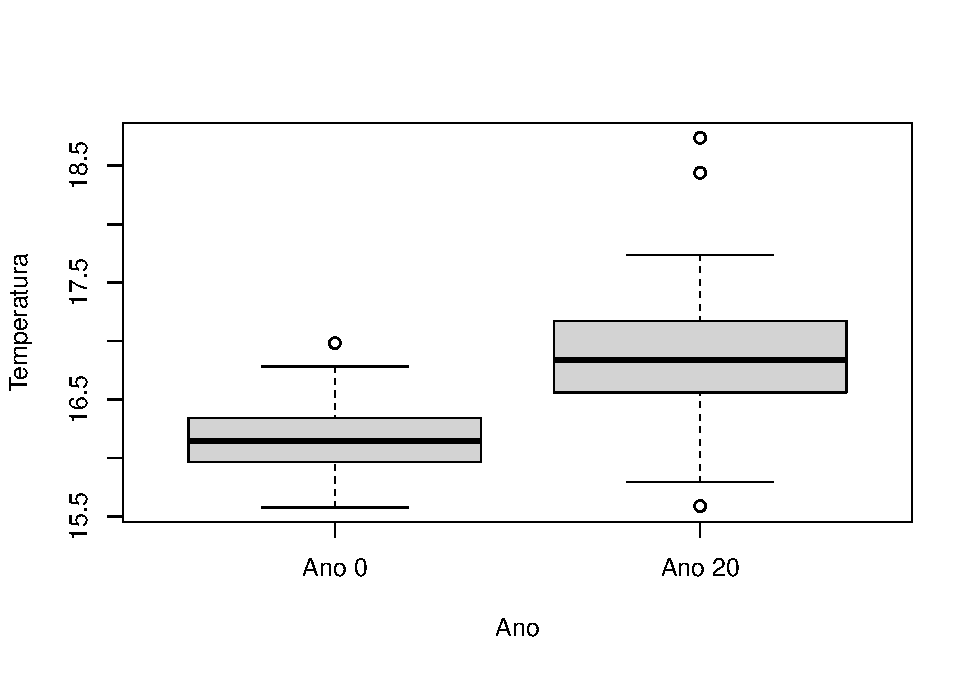
\includegraphics{livroR-1.0_files/figure-latex/box-temp-1.pdf}
\caption{\label{fig:box-temp}Boxplot com os valores de temperatura da lagoa por ano.}
\end{figure}

Como podem verificar os comandos para a análise gráfica não diferiu do que fizemos no exemplo anterior. Os comandos acima realizam: o histograma dos valores de temperatura no ano 0 (Figura \ref{fig:hist-temp-0}), o histograma dos valores de temperatura no ano 0 (Figura \ref{fig:hist-temp-20}) e o boxplot para ambos os dados (Figura \ref{fig:box-temp}), respectivamente. Quanto ao seu resultado podemos notar uma maior temperatura média anual da lagoa 20 anos depois da primeira amostragem.

\begin{Shaded}
\begin{Highlighting}[]
\KeywordTok{summary}\NormalTok{(lagoa)}
\end{Highlighting}
\end{Shaded}

\begin{verbatim}
##      Ano      Temperatura   
##  Ano 0 :36   Min.   :15.58  
##  Ano 20:36   1st Qu.:16.08  
##              Median :16.41  
##              Mean   :16.52  
##              3rd Qu.:16.86  
##              Max.   :18.74
\end{verbatim}

\begin{Shaded}
\begin{Highlighting}[]
\KeywordTok{library}\NormalTok{(Rmisc)}
\KeywordTok{summarySE}\NormalTok{(}\DataTypeTok{data =}\NormalTok{ lagoa, }\DataTypeTok{measurevar =} \StringTok{"Temperatura"}\NormalTok{, }\DataTypeTok{groupvars =} \StringTok{"Ano"}\NormalTok{)}
\end{Highlighting}
\end{Shaded}

\begin{verbatim}
##      Ano  N Temperatura        sd         se        ci
## 1  Ano 0 36    16.14661 0.3301591 0.05502652 0.1117098
## 2 Ano 20 36    16.89750 0.6409853 0.10683089 0.2168782
\end{verbatim}

Aplicando a função \emph{summarySE()} do pacote Rmisc obtivemos sumarizamos nossos dados como mostrado acima e em relação aos valores de média e desvios podemos observar que a média é bem próxima, mas será que elas são estatisticamente iguais? Para isso vamos realizar o teste-t.

Antes do teste vamos calcular os pressupostos do teste, normalidade e homocedasticidade.

\begin{Shaded}
\begin{Highlighting}[]
\KeywordTok{shapiro.test}\NormalTok{(lagoa}\OperatorTok{$}\NormalTok{Temperatura [lagoa}\OperatorTok{$}\NormalTok{Ano }\OperatorTok{==}\StringTok{ "Ano 0"}\NormalTok{])}
\end{Highlighting}
\end{Shaded}

\begin{verbatim}
## 
##  Shapiro-Wilk normality test
## 
## data:  lagoa$Temperatura[lagoa$Ano == "Ano 0"]
## W = 0.97181, p-value = 0.4771
\end{verbatim}

\begin{Shaded}
\begin{Highlighting}[]
\KeywordTok{shapiro.test}\NormalTok{(lagoa}\OperatorTok{$}\NormalTok{Temperatura [lagoa}\OperatorTok{$}\NormalTok{Ano }\OperatorTok{==}\StringTok{ "Ano 20"}\NormalTok{])}
\end{Highlighting}
\end{Shaded}

\begin{verbatim}
## 
##  Shapiro-Wilk normality test
## 
## data:  lagoa$Temperatura[lagoa$Ano == "Ano 20"]
## W = 0.9571, p-value = 0.1747
\end{verbatim}

\begin{Shaded}
\begin{Highlighting}[]
\KeywordTok{bartlett.test}\NormalTok{(Temperatura }\OperatorTok{~}\StringTok{ }\NormalTok{Ano, }\DataTypeTok{data =}\NormalTok{ lagoa)}
\end{Highlighting}
\end{Shaded}

\begin{verbatim}
## 
##  Bartlett test of homogeneity of variances
## 
## data:  Temperatura by Ano
## Bartlett's K-squared = 14.189, df = 1, p-value = 0.0001653
\end{verbatim}

Como podemos ver os dados são normais, porém não são homocedasticos (a variância não é igual entre os grupos). Neste caso podemos fazer um teste-t de Welch (este teste aplica uma correção quando as variâncias não são iguais). Contudo, o teste de Welch ele é comumente usado quando o N amostral é considerado baixo (menor que 10 para um dos dois grupos). Vamos Analisar o teste-t considerando a variância igual e desigual para ver se há diferença significativa no resultado do teste ou não.

\begin{Shaded}
\begin{Highlighting}[]
\KeywordTok{t.test}\NormalTok{(Temperatura }\OperatorTok{~}\StringTok{ }\NormalTok{Ano, }
       \DataTypeTok{data =}\NormalTok{ lagoa,}
       \DataTypeTok{var.equal =} \OtherTok{TRUE}\NormalTok{,}
       \DataTypeTok{conf.level =} \FloatTok{0.99}\NormalTok{)}
\end{Highlighting}
\end{Shaded}

\begin{verbatim}
## 
##  Two Sample t-test
## 
## data:  Temperatura by Ano
## t = -6.2486, df = 70, p-value = 2.837e-08
## alternative hypothesis: true difference in means is not equal to 0
## 99 percent confidence interval:
##  -1.069087 -0.432691
## sample estimates:
##  mean in group Ano 0 mean in group Ano 20 
##             16.14661             16.89750
\end{verbatim}

\begin{Shaded}
\begin{Highlighting}[]
\KeywordTok{t.test}\NormalTok{(Temperatura }\OperatorTok{~}\StringTok{ }\NormalTok{Ano, }
       \DataTypeTok{data =}\NormalTok{ lagoa,}
       \DataTypeTok{var.equal =} \OtherTok{FALSE}\NormalTok{,}
       \DataTypeTok{conf.level =} \FloatTok{0.99}\NormalTok{)}
\end{Highlighting}
\end{Shaded}

\begin{verbatim}
## 
##  Welch Two Sample t-test
## 
## data:  Temperatura by Ano
## t = -6.2486, df = 52.35, p-value = 7.594e-08
## alternative hypothesis: true difference in means is not equal to 0
## 99 percent confidence interval:
##  -1.0721092 -0.4296686
## sample estimates:
##  mean in group Ano 0 mean in group Ano 20 
##             16.14661             16.89750
\end{verbatim}

Como podem notar a forma de escrever o teste é similar ao exemplo anterior as alterações consistem nas variáveis e conjunto de dados utilizado e como foi pedido no teste a alteração do nível de confiança para 99\% (conf.level = 0,99) e os dois teste-t (com variância igual e com variância desigual - Welch).

Olhando para os dois resultados ambos os testes demonstraram diferenças significativas entre os anos, pois o p-value foi menor que 0,01 (lembrar que como o nível de confiança foi alterado para 0,99 a significância só ocorrerá se o p-value for menor que 0,01, como é o caso). Porém podemos ver que não há muita diferença em relação aos valores de ambos os teste-t, pois como comunicamos a aplicação do teste-t de Welch apresenta maior importância quando as variâncias são desiguais e o número amostral de um dos grupos é muito pequeno.

Assim como fizemos anteriormente vamos olhar o resultado em relação a distribuição da função de densidade do teste-t para um nível de confiança de 99\% (Figura \ref{fig:testet-duas-temp-dens}). Só devemos lembrar de carregar o pacote ``webr'' se ainda não foi carregado.

\begin{Shaded}
\begin{Highlighting}[]
\KeywordTok{library}\NormalTok{(webr)}
\KeywordTok{plot}\NormalTok{(}\KeywordTok{t.test}\NormalTok{(Temperatura }\OperatorTok{~}\StringTok{ }\NormalTok{Ano, }
            \DataTypeTok{data =}\NormalTok{ lagoa,}
            \DataTypeTok{var.equal =} \OtherTok{TRUE}\NormalTok{,}
            \DataTypeTok{conf.level =} \FloatTok{0.99}\NormalTok{))}
\end{Highlighting}
\end{Shaded}

\begin{figure}
\centering
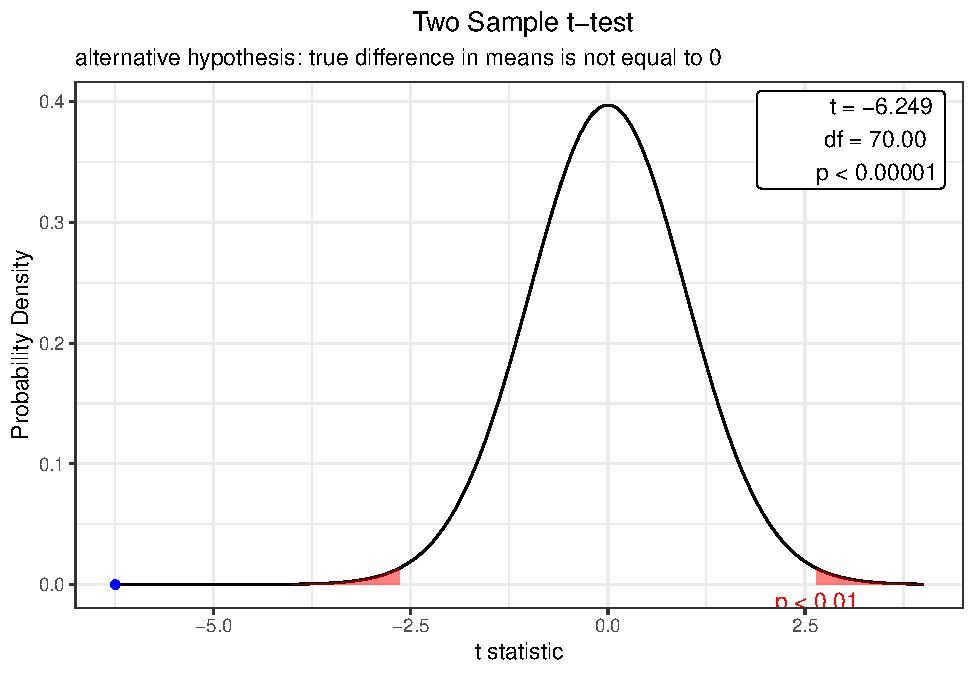
\includegraphics{livroR-1.0_files/figure-latex/testet-duas-temp-dens-1.pdf}
\caption{\label{fig:testet-duas-temp-dens}Curva de densidade representando o valor do teste-t bicaudal para comparação da temperatura em um lago entre dois anos a um intervalo de confiança de 99\%. O ponto azul indica o valor do teste.}
\end{figure}

De acordo com esse exemplo podemos afirmar que os anos diferem entre si e que em 20 anos a lagoa amostrada apresentou um aumento da temperatura.

\hypertarget{teste-t-pareado}{%
\section{Teste-t pareado}\label{teste-t-pareado}}

Aplicamos este teste quando as duas amostras de uma variável categórica são independentes e desejamos verificar se elas são similares entre si. Contudo cada observação de ambas as amostras devem de alguma forma estar associadas para podermos dizer que ocorrem em pares. Neste caso as hipóteses são as seguintes:

H0: Não há diferença entre os pares de observações;

HA: Há diferença entre os pares de observações;

Matematicamente pode ser dita da seguinte forma:

H0: A diferença na média dos pares de observações é igual a 0;

HA: A diferença na média dos pares de observações é diferente de 0;

Vejamos um exemplo de como conduzir essa análise no R

Imagine que dois pesquisadores embarcaram com objetivo de fazer contagem de aves em alto mar. Após 20 dias de observações independentes entre os observadores obtivemos os dados abaixo.

Começaremos gerando os dados e a modificando se necessário.

\begin{Shaded}
\begin{Highlighting}[]
\NormalTok{observadores <-}\StringTok{ }\KeywordTok{c}\NormalTok{(}\KeywordTok{rep}\NormalTok{(}\DataTypeTok{x =} \StringTok{"Observador 1"}\NormalTok{, }\DecValTok{20}\NormalTok{), }\KeywordTok{rep}\NormalTok{(}\DataTypeTok{x =} \StringTok{"Observador 2"}\NormalTok{, }\DecValTok{20}\NormalTok{))}
\KeywordTok{set.seed}\NormalTok{(}\DecValTok{2328}\NormalTok{)}
\NormalTok{aves}\FloatTok{.1}\NormalTok{ <-}\StringTok{ }\KeywordTok{rnorm}\NormalTok{(}\DataTypeTok{n =} \DecValTok{20}\NormalTok{, }\DataTypeTok{mean =} \DecValTok{20}\NormalTok{, }\DataTypeTok{sd =} \DecValTok{1}\NormalTok{) }\OperatorTok{+}\StringTok{ }\KeywordTok{runif}\NormalTok{(}\DataTypeTok{n =} \DecValTok{20}\NormalTok{)}
\KeywordTok{set.seed}\NormalTok{(}\DecValTok{3230}\NormalTok{)}
\NormalTok{aves}\FloatTok{.2}\NormalTok{ <-}\StringTok{ }\KeywordTok{rnorm}\NormalTok{(}\DataTypeTok{n =} \DecValTok{20}\NormalTok{, }\DataTypeTok{mean =} \DecValTok{21}\NormalTok{, }\DataTypeTok{sd =} \DecValTok{2}\NormalTok{) }\OperatorTok{+}\StringTok{ }\KeywordTok{runif}\NormalTok{(}\DataTypeTok{n =} \DecValTok{20}\NormalTok{)}
\NormalTok{dia <-}\StringTok{ }\KeywordTok{c}\NormalTok{(}\StringTok{"Dia 1"}\NormalTok{, }\StringTok{"Dia 2"}\NormalTok{, }\StringTok{"Dia 3"}\NormalTok{, }\StringTok{"Dia 4"}\NormalTok{, }\StringTok{"Dia 5"}\NormalTok{, }\StringTok{"Dia 6"}\NormalTok{, }\StringTok{"Dia 7"}\NormalTok{, }\StringTok{"Dia 8"}\NormalTok{, }\StringTok{"Dia 9"}\NormalTok{, }\StringTok{"Dia 10"}\NormalTok{, }\StringTok{"Dia 11"}\NormalTok{, }\StringTok{"Dia 12"}\NormalTok{, }\StringTok{"Dia 13"}\NormalTok{, }\StringTok{"Dia 14"}\NormalTok{, }\StringTok{"Dia 15"}\NormalTok{, }\StringTok{"Dia 16"}\NormalTok{, }\StringTok{"Dia 17"}\NormalTok{, }\StringTok{"Dia 18"}\NormalTok{, }\StringTok{"Dia 19"}\NormalTok{, }\StringTok{"Dia 20"}\NormalTok{)}
\NormalTok{aves <-}\StringTok{ }\KeywordTok{c}\NormalTok{(aves}\FloatTok{.1}\NormalTok{, aves}\FloatTok{.2}\NormalTok{)}
\NormalTok{aves <-}\StringTok{ }\KeywordTok{as.data.frame}\NormalTok{(}\KeywordTok{cbind}\NormalTok{(dia, }\KeywordTok{round}\NormalTok{(aves}\FloatTok{.1}\NormalTok{, }\DecValTok{0}\NormalTok{), }\KeywordTok{round}\NormalTok{(aves}\FloatTok{.2}\NormalTok{, }\DecValTok{0}\NormalTok{)))}
\KeywordTok{colnames}\NormalTok{(aves) <-}\StringTok{ }\KeywordTok{c}\NormalTok{(}\StringTok{"Dia"}\NormalTok{, }\StringTok{"Observador 1"}\NormalTok{, }\StringTok{"Observador 2"}\NormalTok{)}
\KeywordTok{rm}\NormalTok{(}\DataTypeTok{list =} \StringTok{"observadores"}\NormalTok{, }\StringTok{"aves.1"}\NormalTok{, }\StringTok{"aves.2"}\NormalTok{, }\StringTok{"dia"}\NormalTok{)}
\end{Highlighting}
\end{Shaded}

\textcolor{red}{Neste momento não entraremos em detalhes sobre os comandos aplicados para construção desses dados. Caso seja do seu interesse consulte o apêndice, no final do livro.}

\begin{Shaded}
\begin{Highlighting}[]
\KeywordTok{head}\NormalTok{(aves)}
\end{Highlighting}
\end{Shaded}

\begin{verbatim}
##     Dia Observador 1 Observador 2
## 1 Dia 1           19           20
## 2 Dia 2           20           22
## 3 Dia 3           18           23
## 4 Dia 4           22           18
## 5 Dia 5           22           22
## 6 Dia 6           22           23
\end{verbatim}

\begin{Shaded}
\begin{Highlighting}[]
\KeywordTok{str}\NormalTok{(aves)}
\end{Highlighting}
\end{Shaded}

\begin{verbatim}
## 'data.frame':    20 obs. of  3 variables:
##  $ Dia         : chr  "Dia 1" "Dia 2" "Dia 3" "Dia 4" ...
##  $ Observador 1: chr  "19" "20" "18" "22" ...
##  $ Observador 2: chr  "20" "22" "23" "18" ...
\end{verbatim}

\begin{Shaded}
\begin{Highlighting}[]
\NormalTok{aves}\OperatorTok{$}\NormalTok{Dia <-}\StringTok{ }\KeywordTok{as.factor}\NormalTok{(aves}\OperatorTok{$}\NormalTok{Dia)}
\NormalTok{aves}\OperatorTok{$}\StringTok{`}\DataTypeTok{Observador 1}\StringTok{`}\NormalTok{ <-}\StringTok{ }\KeywordTok{as.numeric}\NormalTok{(aves}\OperatorTok{$}\StringTok{`}\DataTypeTok{Observador 1}\StringTok{`}\NormalTok{)}
\NormalTok{aves}\OperatorTok{$}\StringTok{`}\DataTypeTok{Observador 2}\StringTok{`}\NormalTok{ <-}\StringTok{ }\KeywordTok{as.numeric}\NormalTok{(aves}\OperatorTok{$}\StringTok{`}\DataTypeTok{Observador 2}\StringTok{`}\NormalTok{)}
\KeywordTok{str}\NormalTok{(aves)}
\end{Highlighting}
\end{Shaded}

\begin{verbatim}
## 'data.frame':    20 obs. of  3 variables:
##  $ Dia         : Factor w/ 20 levels "Dia 1","Dia 10",..: 1 12 14 15 16 17 18 19 20 2 ...
##  $ Observador 1: num  19 20 18 22 22 22 21 20 22 21 ...
##  $ Observador 2: num  20 22 23 18 22 23 20 24 22 24 ...
\end{verbatim}

Agora definimos nossas hipóteses

H0: Não há diferença entre os pares de observações dos pesquisadores;

HA: Há diferença entre os pares de observações dos pesquisadores;

Vamos sumarizar os dados gráfica e estatisticamente

\begin{Shaded}
\begin{Highlighting}[]
\KeywordTok{hist}\NormalTok{(aves}\OperatorTok{$}\StringTok{`}\DataTypeTok{Observador 1}\StringTok{`}\NormalTok{, }
     \DataTypeTok{xlab =} \StringTok{"Observações"}\NormalTok{, }
     \DataTypeTok{ylab =} \StringTok{"Frequência", }
\StringTok{     main = "}\NormalTok{Observador }\DecValTok{1}\StringTok{", }
\StringTok{     ylim = c(0, 10),}
\StringTok{     xlim = c(18, 25))}
\end{Highlighting}
\end{Shaded}

\begin{figure}
\centering
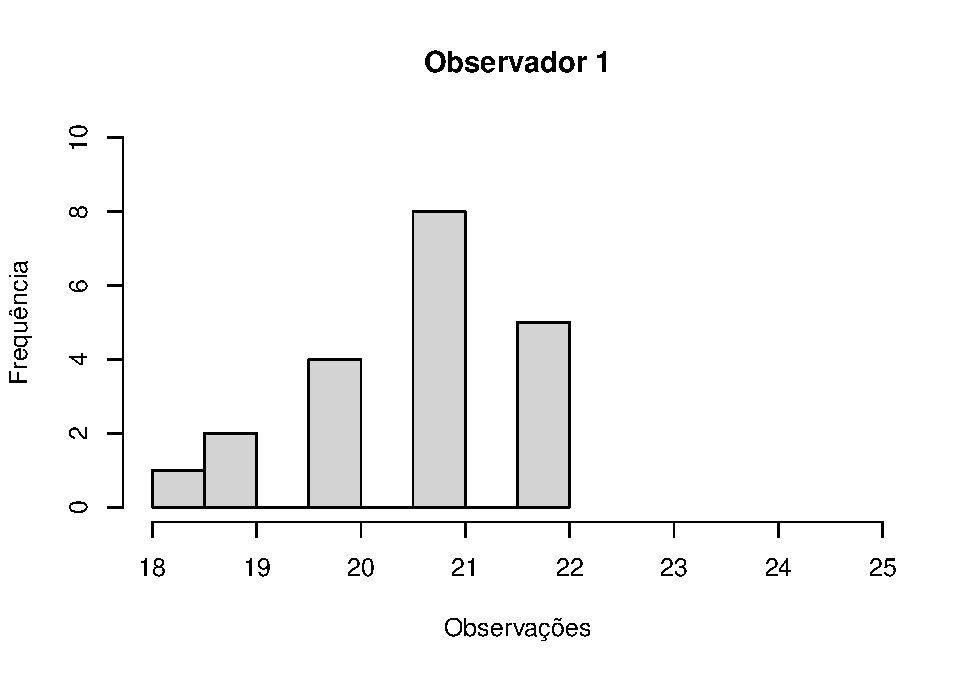
\includegraphics{livroR-1.0_files/figure-latex/hist-par-obs1-1.pdf}
\caption{\label{fig:hist-par-obs1}Histograma com a frequência de observações de aves, por 20 dias, pelo observador 1}
\end{figure}

\begin{Shaded}
\begin{Highlighting}[]
\KeywordTok{hist}\NormalTok{(aves}\OperatorTok{$}\StringTok{`}\DataTypeTok{Observador 2}\StringTok{`}\NormalTok{, }
     \DataTypeTok{xlab =} \StringTok{"Observações"}\NormalTok{, }
     \DataTypeTok{ylab =} \StringTok{"Frequência", }
\StringTok{     main = "}\NormalTok{Observador }\DecValTok{2}\StringTok{", }
\StringTok{     ylim = c(0, 10),}
\StringTok{     xlim = c(18, 25))}
\end{Highlighting}
\end{Shaded}

\begin{figure}
\centering
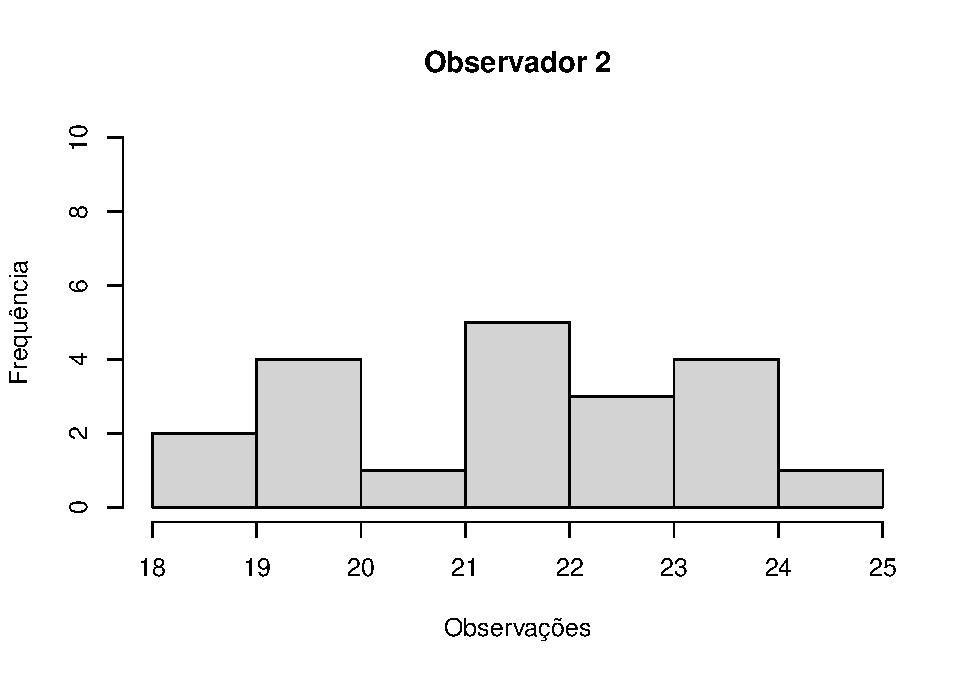
\includegraphics{livroR-1.0_files/figure-latex/hist-par-obs2-1.pdf}
\caption{\label{fig:hist-par-obs2}Histograma com a frequência de observações de aves, por 20 dias, pelo observador 2}
\end{figure}

\begin{Shaded}
\begin{Highlighting}[]
\KeywordTok{boxplot}\NormalTok{(aves}\OperatorTok{$}\StringTok{`}\DataTypeTok{Observador 1}\StringTok{`}\NormalTok{, }
\NormalTok{        aves}\OperatorTok{$}\StringTok{`}\DataTypeTok{Observador 2}\StringTok{`}\NormalTok{, }
        \DataTypeTok{names =} \KeywordTok{c}\NormalTok{(}\StringTok{"Observador 1"}\NormalTok{, }\StringTok{"Observador 2"}\NormalTok{),}
        \DataTypeTok{ylab =} \StringTok{"Frequência de Observações"}\NormalTok{)}
\end{Highlighting}
\end{Shaded}

\begin{figure}
\centering
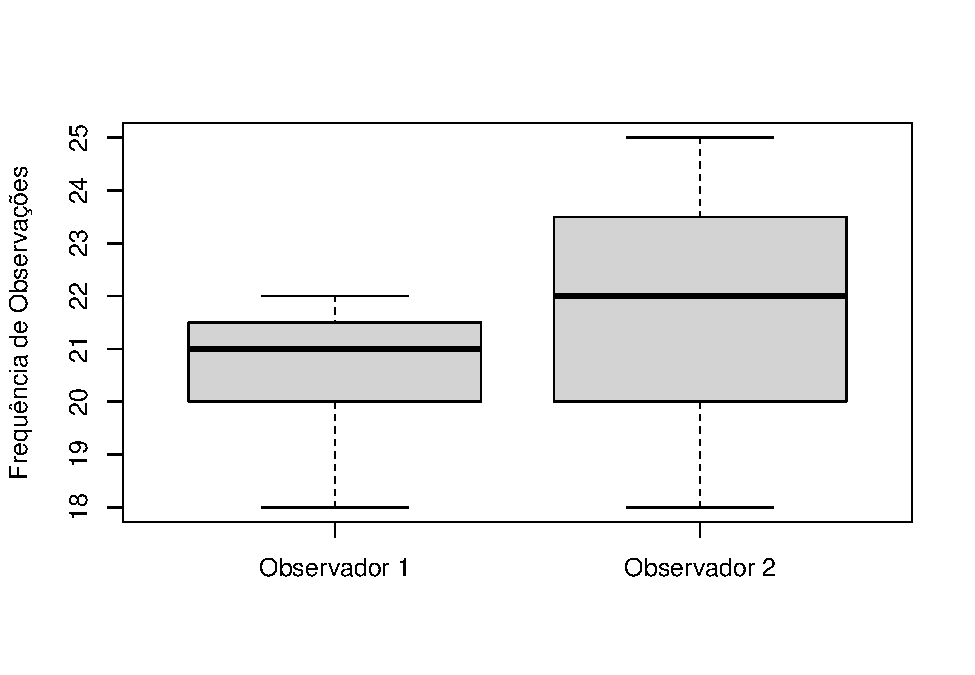
\includegraphics{livroR-1.0_files/figure-latex/box-par-ave-1.pdf}
\caption{\label{fig:box-par-ave}Boxplot com as frequências de observações de aves por 20 dias de 2 observadores.}
\end{figure}

Como podem verificar os comandos para a análise gráfica não diferiu do que fizemos nos exemplos anteriores para os histogramas (Figura \ref{fig:hist-par-obs1} e \ref{fig:hist-par-obs2}) e pouco diferiu para o boxplot ((Figura \ref{fig:box-par-ave}).

A estrutura da planilha é diferente das anteriores o que por sua vez alterou a mudança na escrita do comando para construção para o boxplot. Desta não mais utilizamos o til (\textasciitilde{}), mas inserimos o nome da planilha seguido pelo operador matemático \$ (cifrão) mais o nome da variável quantitativa que queremos representar. Inserimos também outros 2 argumentos que são ``names'' com dois nomes concatenados pela função c() que representam as variáveis quantitativas na ordem em que foram inseridas e o argumento ``ylab'' que dá nome ao eixo y.

\begin{Shaded}
\begin{Highlighting}[]
\KeywordTok{summary}\NormalTok{(aves)}
\end{Highlighting}
\end{Shaded}

\begin{verbatim}
##       Dia      Observador 1    Observador 2  
##  Dia 1  : 1   Min.   :18.00   Min.   :18.00  
##  Dia 10 : 1   1st Qu.:20.00   1st Qu.:20.00  
##  Dia 11 : 1   Median :21.00   Median :22.00  
##  Dia 12 : 1   Mean   :20.70   Mean   :21.90  
##  Dia 13 : 1   3rd Qu.:21.25   3rd Qu.:23.25  
##  Dia 14 : 1   Max.   :22.00   Max.   :25.00  
##  (Other):14
\end{verbatim}

Como podemos notar, devido a organização dos dados na planilha a função \emph{summary()} já sumariza de maneira adequada nossos dados.

Em relação ao resumo dos nossos dados podemos observar que o observador 2 contabilizou um número maior de aves que o observador 1, mas será que a diferença no número de observações é nulo (0) ou é diferente. ou seja será que a média de observação entre os observadores é similar?

O teste-t pareado não aparesenta pressuposto quanto aos dados, porém como ele avalia a diferença entre dois grupos o pressuposto requerido é a normalidade da diferença dos dados. Vamos a nossa avaliação do pressuposto.

Primeiro vamos criar um objeto que consiste na diferença entre observadores

\begin{Shaded}
\begin{Highlighting}[]
\NormalTok{diferenca <-}\StringTok{ }\NormalTok{aves}\OperatorTok{$}\StringTok{`}\DataTypeTok{Observador 1}\StringTok{`} \OperatorTok{-}\StringTok{ }\NormalTok{aves}\OperatorTok{$}\StringTok{`}\DataTypeTok{Observador 2}\StringTok{`}
\end{Highlighting}
\end{Shaded}

Agora vamos realizar o teste de normalidade da diferença.

\begin{Shaded}
\begin{Highlighting}[]
\KeywordTok{shapiro.test}\NormalTok{(diferenca)}
\end{Highlighting}
\end{Shaded}

\begin{verbatim}
## 
##  Shapiro-Wilk normality test
## 
## data:  diferenca
## W = 0.98173, p-value = 0.9544
\end{verbatim}

De acordo com o teste de Shapiro os dados são normais. Vamos a nossa avaliação pelo teste-t

\begin{Shaded}
\begin{Highlighting}[]
\KeywordTok{t.test}\NormalTok{(aves}\OperatorTok{$}\StringTok{`}\DataTypeTok{Observador 1}\StringTok{`}\NormalTok{,}
\NormalTok{       aves}\OperatorTok{$}\StringTok{`}\DataTypeTok{Observador 2}\StringTok{`}\NormalTok{,}
       \DataTypeTok{paired =} \OtherTok{TRUE}\NormalTok{,}
       \DataTypeTok{conf.level =} \FloatTok{0.95}\NormalTok{)}
\end{Highlighting}
\end{Shaded}

\begin{verbatim}
## 
##  Paired t-test
## 
## data:  aves$`Observador 1` and aves$`Observador 2`
## t = -2.1608, df = 19, p-value = 0.04369
## alternative hypothesis: true difference in means is not equal to 0
## 95 percent confidence interval:
##  -2.36237491 -0.03762509
## sample estimates:
## mean of the differences 
##                    -1.2
\end{verbatim}

Para a execução do teste-t pareado 2 diferenças podem ser notadas na escrita da função. A primeira consiste no fato de que não utilizamos o til (\textasciitilde{}), mas sim as variáveis referentes as observações e a segunda é o argumento paired que tem valor lógico (ou seja, verdadeiro ou falso) e indicamos ele como ``TRUE'' (verdadeiro).

Quanto ao resultado podemos notar que nos é informado que o teste consiste num teste-t pareado e que a diferença entre os observadores é ligeiramente diferente a um nível de confiança de 95\%, visto que o ``p-value'' é próximo à 0,05 e na última linha nos é indicado que a média da diferença das observações é de -1,2. Em outras palavras o teste nos diz que a média das diferenças é diferente de 0, portanto rejeitamos a hipótese nula.

Assim como fizemos anteriormente vamos olhar o resultado em relação a distribuição função de densidade do teste-t (Figura \ref{fig:testet-par-ave}). Só devemos lembrar de carregar o pacote ``webr'' se ainda não foi carregado.

\begin{Shaded}
\begin{Highlighting}[]
\KeywordTok{library}\NormalTok{(webr)}
\KeywordTok{plot}\NormalTok{(}\KeywordTok{t.test}\NormalTok{(aves}\OperatorTok{$}\StringTok{`}\DataTypeTok{Observador 1}\StringTok{`}\NormalTok{,}
\NormalTok{            aves}\OperatorTok{$}\StringTok{`}\DataTypeTok{Observador 2}\StringTok{`}\NormalTok{,}
            \DataTypeTok{paired =} \OtherTok{TRUE}\NormalTok{,}
            \DataTypeTok{conf.level =} \FloatTok{0.95}\NormalTok{))}
\end{Highlighting}
\end{Shaded}

\begin{figure}
\centering
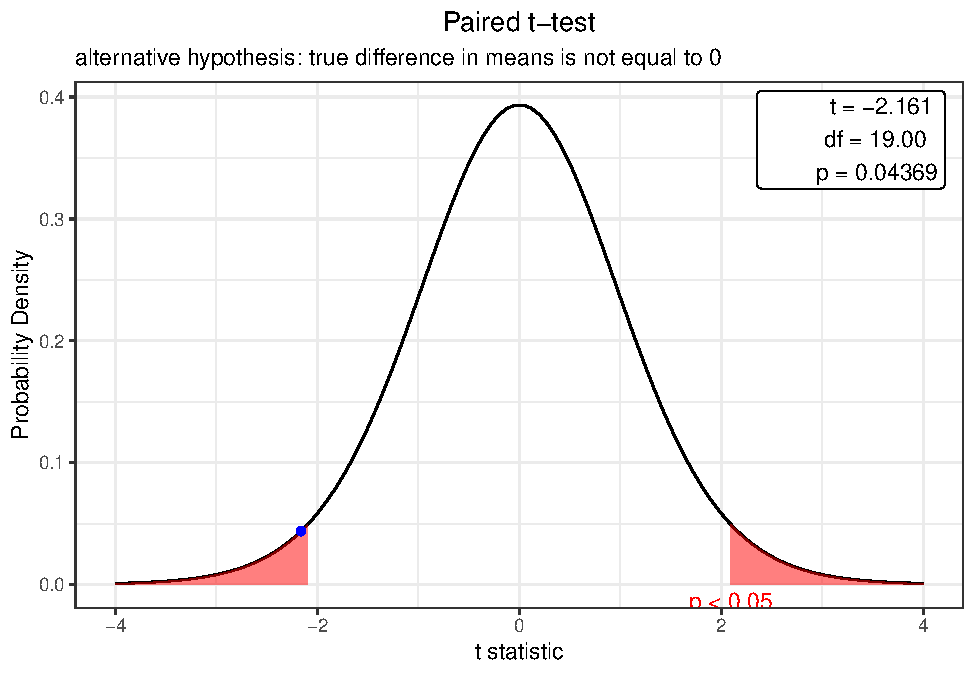
\includegraphics{livroR-1.0_files/figure-latex/testet-par-ave-1.pdf}
\caption{\label{fig:testet-par-ave}Curva de densidade representando o valor do teste-t bicaudal para comparação do número de observações de aves por 2 observadores distintos a um intervalo de confiança de 95\%. O ponto azul indica o valor do teste.}
\end{figure}

Neste teste em particular como trabalhamos com a diferença entre as observações vamos usar o gráfico de barras para graficar essa diferença.

\begin{Shaded}
\begin{Highlighting}[]
\KeywordTok{barplot}\NormalTok{(diferenca,}
        \DataTypeTok{xlab =} \StringTok{"Dias"}\NormalTok{,}
        \DataTypeTok{ylab =} \StringTok{"Diferença entre observadores (Observador 1 - Observador 2)"}\NormalTok{,}
        \DataTypeTok{main =} \StringTok{"Meu gráfico"}\NormalTok{,}
        \DataTypeTok{names.arg =}\NormalTok{ aves}\OperatorTok{$}\NormalTok{Dia,}
        \DataTypeTok{las =} \DecValTok{2}\NormalTok{,}
        \DataTypeTok{ylim =} \KeywordTok{c}\NormalTok{(}\OperatorTok{-}\FloatTok{7.3}\NormalTok{, }\FloatTok{7.3}\NormalTok{),}
        \DataTypeTok{cex.names =} \FloatTok{0.9}\NormalTok{)}
\end{Highlighting}
\end{Shaded}

\begin{figure}
\centering
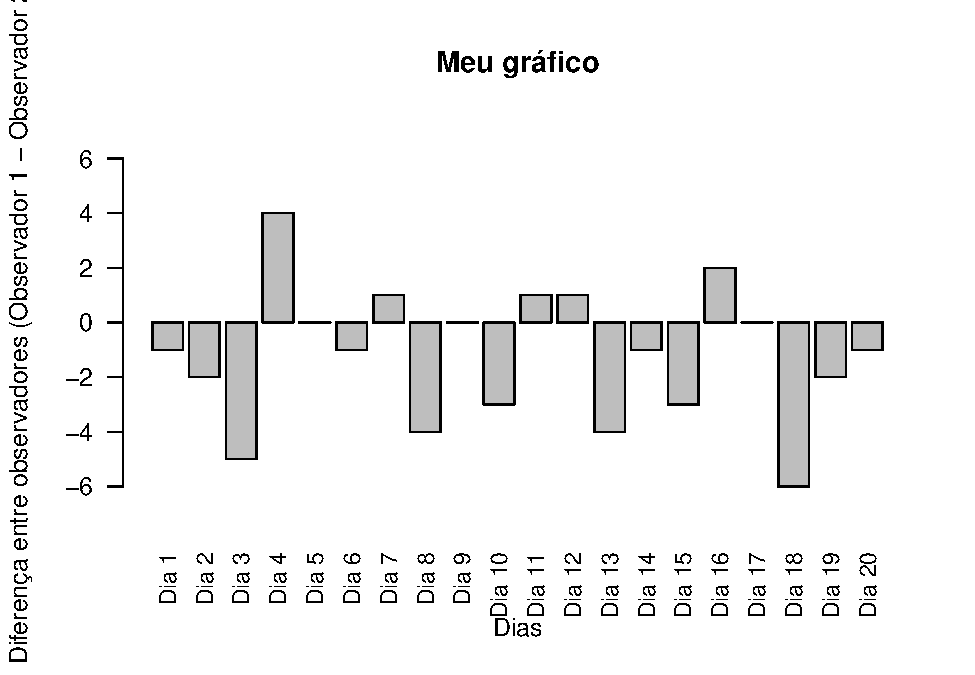
\includegraphics{livroR-1.0_files/figure-latex/bar-dif-ave-1.pdf}
\caption{\label{fig:bar-dif-ave}Diferença entre o número de observações de aves, por dia, para cada observador}
\end{figure}

Para o gráfico acima indicamos em seu comando que faremos um gráfico de barras onde o que será plotado é a diferença no número de observação de aves entre observadores (Figura \ref{fig:bar-dif-ave}). O argumento ``xlab'' indica o nome do eixo x, ``ylab'' o nome do eixo y, ``main'' indica o título do gráfico, ``names.arg'' indica a coluna referente aos nomes das barras (que são os dias), ``las'' indica se os nomes das barras serão plotados na horizontal ou vertical (o valor 2 indica vertical), ``ylim'' indica os limites do eixo y e ``cex.names'' indica o tamanho da letra dos nomes das barras.

As barras para o lado positivo do eixo y indica uma maior observação de aves pelo observador 1 e as barras para baixo indicam um maior número de observações de aves pelo observador 2. Vamos indicar isso no gráfico por meio da função \emph{mtext()} (Figura \ref{fig:bar-dif-ave2}).

\begin{Shaded}
\begin{Highlighting}[]
\KeywordTok{barplot}\NormalTok{(diferenca,}
        \DataTypeTok{xlab =} \StringTok{"Dias"}\NormalTok{,}
        \DataTypeTok{ylab =} \StringTok{"Diferença entre observadores (Observador 1 - Observador 2)"}\NormalTok{,}
        \DataTypeTok{main =} \StringTok{"Meu gráfico"}\NormalTok{,}
        \DataTypeTok{names.arg =}\NormalTok{ aves}\OperatorTok{$}\NormalTok{Dia,}
        \DataTypeTok{las =} \DecValTok{2}\NormalTok{,}
        \DataTypeTok{ylim =} \KeywordTok{c}\NormalTok{(}\OperatorTok{-}\FloatTok{7.3}\NormalTok{, }\FloatTok{7.3}\NormalTok{),}
        \DataTypeTok{cex.names =} \FloatTok{0.9}\NormalTok{)}

\KeywordTok{mtext}\NormalTok{(}\DataTypeTok{at =} \DecValTok{4}\NormalTok{,}
      \DataTypeTok{line =} \DecValTok{-2}\NormalTok{,}
      \DataTypeTok{text =} \StringTok{"Observador 1"}\NormalTok{, }
      \DataTypeTok{side =} \DecValTok{3}\NormalTok{)}
\KeywordTok{mtext}\NormalTok{(}\DataTypeTok{at =} \DecValTok{4}\NormalTok{, }
      \DataTypeTok{line =} \DecValTok{-2}\NormalTok{,}
      \DataTypeTok{text =} \StringTok{"Observador 2"}\NormalTok{, }
      \DataTypeTok{side =} \DecValTok{1}\NormalTok{)}
\end{Highlighting}
\end{Shaded}

\begin{figure}
\centering
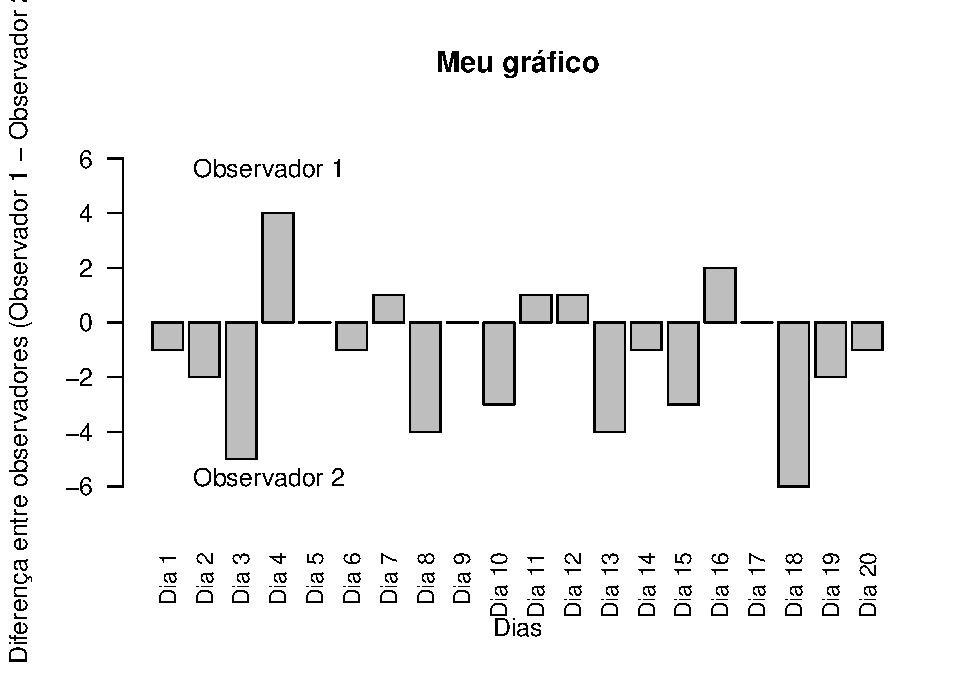
\includegraphics{livroR-1.0_files/figure-latex/bar-dif-ave2-1.pdf}
\caption{\label{fig:bar-dif-ave2}Diferença entre o número de observações de aves, por dia, para cada observador.}
\end{figure}

Como podem ver a função \emph{mtext()} indicou os nomes Observador 1 e Observador 2 no lado do gráfico que os representa. O argumento ``at'' indica a posição em relação ao eixo x, ``line'' indica a posição em relação ao eixo y, ``text'' indica o que será plotado e side indica o lado da janela gráfica onde o texto será plotado (3 é na parte superior e 1 na inferior).

\hypertarget{final-words}{%
\chapter{Final Words}\label{final-words}}

We have finished a nice book.

\bibliography{book.bib,packages.bib}

\end{document}
